\documentclass{beamer}

\usepackage{amssymb} 
\usepackage{amsmath} % This is the file main.tex \usepackage{multimedia} 
\usepackage{graphicx}
\hypersetup{colorlinks,linkcolor=blue,urlcolor=blue} 
\usepackage{hyperref}
\usepackage{epstopdf}
\usepackage{caption}
\usepackage{adjustbox}

%%%%%%%%% NEW COMMAND MACRO %%%%%%%%%%%%%%%%%%%%%%%%%%%%%%

\newcommand{\notorth}{\ensuremath{\perp\!\!\!\!\!\!\diagup\!\!\!\!\!\!\perp}}
\newcommand{\orth}{\ensuremath{\perp\!\!\!\perp}}

%%%%%%%%% Theme %%%%%%%%%%%%%%%%%%%%%%%%%%%%%%%%%%%%%%%%%%%%%%%%%

%\usetheme{Warsaw}
\usetheme{Boadilla}
% or ...

\usecolortheme{orchid}
%\usecolortheme[Blue]{structure}
% Alternatively, you can try Copenhagen; its borders are slightly less dark, but its the same style (rounded edged rectangle on the first %slide)
%\usetheme{Copenhagen}

%% Whatever is on the top of the slide
%\useinnertheme{rounded} %%rectangles, circles, rounded, inmargin, 
%\useoutertheme{split} %%puts sections on the upper-left hand side and subsections in upper-rhs; name and title on 

\setbeamerfont{table}{size=\footnotesize} 
\setbeamerfont{smalltable}{size=\scriptsize} 
\setbeamerfont{microtable}{size=\tiny}
\setbeamertemplate{navigation symbols}{}  %%Get rid of the navigation symbols at the bottom
\setbeamertemplate{footline}[text line]{\parbox{\linewidth}{\hfill  \insertpagenumber / \insertpresentationendpage}} %\insertshortauthor \hspace{2ex} \insertshorttitle
%\setbeamertemplate{footline}[text line]{\parbox{\linewidth}{\vspace*{-8pt}\insertshortauthor  \hfill  \insertpagenumber }}  %\insertpresentationendpage

\usepackage{booktabs}
\usepackage[flushleft]{threeparttable}


%Here is alternative table of contents pointers% 
%\setbeamertemplate{sections/subsections in toc}[square] 
\setbeamertemplate{sections/subsections in toc}[circle] 
%\setbeamertemplate{sections/subsections in toc}[ball] 
%\setbeamertemplate{sections/subsections in toc}[ball unnumbered]
%\setbeamertemplate{sections/subsections in toc}[default]

%The next line is the background. Right now we have it set to a vertical shading, with top white bottom 20% blue. 
%You can alter this however you want. We were using red!20 before. You can use standard names for colors, or if I understand correctly 
%you can also use RGB (red green blue) code, for example 30,30,30) 
%\setbeamertemplate{background canvas}[vertical shading][top=white,bottom=blue!10]

%Alternatively, you can make the background just a solid color. 
%\setbeamercolor{background canvas}{bg=red!5}

%Below is the amount of opaqueness in terms of percent.  You can remove this line or set to 0 and it will make future lines unable to be seen.
\setbeamercovered{transparent=15}

%%%%%%%%%%%%%%%%%%%%%%%%%%%%%%%%%%%%%%%%%%%%%%%%%%%%%%%%%%%%%%%%%%%%%%%%%%%%%%%

\title[Reggio Children Approach]{Evaluating the impact of infant-toddler centers and preschools} 
\bigskip
\subtitle{The Reggio Children Approach}
%\usebeamerfont{smalltable}

\begin{document}

\maketitle

%\AtBeginSection[]   {\frame<beamer>{\frametitle{Outline}\tableofcontents[currentsection,currentsubsection]}}
\AtBeginSubsection[]{\frame<beamer>{\frametitle{Outline}\tableofcontents[currentsection,currentsubsection]}}

\section{Introduction}\label{sec:Intro}
\subsection{Question}\label{sec:question}
%%------------------------------------------------------------------------------------------------------- 
\begin{frame}
%\frametitle{Should we invest in preschool education?} 
\frametitle{Research Question} 

\begin{block}{Research Question}
Does high quality preschool improve children outcomes?
\end{block}

\vspace{2ex}

\begin{itemize}
	\item High Quality: Reggio Children Approach
	\begin{itemize}
		\item Innovative pedagogical approach
		\item Scalable
		\item Publicly funded
	\end{itemize}
	\item Outcomes:
	\begin{itemize}
		\item Socio-emotional skills
		\item Mental health
		\item Overall health
	\end{itemize}
%\end{itemize}

%\pause
\vspace{4ex}

%\textbf{Why} do we care?
%\begin{itemize}
%%\item Scattered evidence of impact of early childcare
%\item Increasing demand for early childcare (maternal employment)
%\item How to best use public money in education?
%\item Can positive results from small-scale RCT be scaled up?
%
%\vspace{2ex}

\item[$\hookrightarrow$] Use newly collected data to answer this question 
\end{itemize}


\end{frame} 

%%------------------------------------------------------------------------------------------------------- 
\subsection{Background}\label{sec:Back}
%%------------------------------------------------------------------------------------------------------- 
\begin{frame}
\frametitle{The Reggio Children Approach to Early Childhood Education} 
\begin{itemize}
	\item Natural experiment started 50 years ago in Reggio Emilia
	\begin{itemize}
		\item Innovative pedagogical approach %(Loris Malaguzzi)
		\item One of the first public preschool in Italy (post WWII)
	\end{itemize}
	\item Comprehensive program, age 0-6 
	\item High-quality 
	\item Low-cost
	\item Scalable in size and sustainable
	\item Span across social and economic classes
\end{itemize}
\end{frame} 

%%----------------------------------------------------------------------------------------------- 
\begin{frame}
\frametitle{The Reggio Children Approach - Philosophy}\label{frame:philosphy}
%\usebeamerfont{table}
\begin{itemize}
	\item Educational philosophy started by \textbf{Loris Malaguzzi} after WWII.
	\item First preschool 1963; first infant-toddler center 1972 \hyperlink{fig:Num_Nidi}{\beamergotobutton{evolution}}
	\item Famous and replicated all over the world \hyperlink{fig:World}{\beamergotobutton{map}}
	\item 26 Infant-toddler centers and 30 preschools

	\vspace{2ex}

%	\item Principle: three main pillars
%	\begin{enumerate}
%		\item The organization of the class and the training and collegial work for all educational figures.
%		\item The central role of children and the important role of families.
%		\item A strong creative, aesthetic and environmental dimension.
%	\end{enumerate}

	\item The Reggio Children Approach principles:
		\begin{itemize}
		\item Develop `100 languages' of children
		\item Child-centered philosophy: children direct learning
		\item Teacher, atelierista, and staff continuously training
		\item School and classroom make `learning visible'
		\item Family and community integrated in learning
		\end{itemize} 
\end{itemize} 
\end{frame} 
%%----------------------------------------------------------------------------------------------- 
\begin{frame}
\frametitle{Early Childhood Education in Italy}\label{frame:ECE_IT}
%\usebeamerfont{table}
\begin{itemize}
	\item 4 institutional types: \hyperlink{fig:PrivateAsiloIT}{\beamergotobutton{asilo}}
	\begin{enumerate}
		\item Municipal
		\item State
		\item Religious
		\item Private
	\end{enumerate}
	\vspace{1ex}
	\item 2 age groups: \hyperlink{fig:AttendaceAsiloIT}{\beamergotobutton{asilo}}
	\begin{enumerate}
		\item Age 0-3: 13\% attendance rate (\textit{asilo nido})
		\item Age 3-6: 94\% attendance rate (\textit{scuola materna})
	\end{enumerate}
	
	\vspace{3ex}
	
	\item[] Reggio Children Approach: \textbf{municipal} infant-toddler centers and preschools \textbf{(age 0-6)} in \textbf{Reggio Emilia}
\end{itemize} 
\end{frame} 
%%-----------------------------------------------------------------------------------------------

%\subsection{The Reggio Children Approach}\label{sec:RCH}
%%%----------------------------------------------------------------------------------------------- 
%\begin{frame}
%\frametitle{The Reggio Children Approach}\label{frame:reggiostyle}
%%\usebeamerfont{table}
%\begin{itemize}
%	\item Reggio Children Approach: educational philosophy started by \textbf{Loris Malaguzzi} after World War II.
%	\item Innovators in Italy: started in 1963 vs. mid 1970s in Parma and Padova
%	\item Low cost:
%	\begin{itemize}
%		\item For families: sliding schedule based on income. Cheaper than State and Religious (slightly) and private (a lot)
%		\item For the public: union teachers' wages
%	\end{itemize}
%	%\item Famous and replicated all over the world \hyperlink{fig:World}{\beamergotobutton{map}}
%	\vspace{2ex}
%	\item The Reggio Children Approach uniqueness:
%		\begin{itemize}
%		\item Child-centered philosophy: child guides the learning
%		\item Develop the `100 languages' of children
%		\item Co-teaching
%		\item Atelieristas and cooks are also teachers
%		\item Family and Community are integrated in learning process
%		\item Longer daily hours
%%		\usebeamerfont{smalltable}
%%		\item Children as a group direct the learning process
%%		\item Develop `100 languages' of children
%%		\item Family integral part of education
%%		\item Teacher and staff continuosly training
%%		\item School and classroom make `learning visible'
%		\end{itemize} 
%\end{itemize} 
%\end{frame} 

\section{Evaluation}\label{sec:Eval}
\subsection{Data}
%%-----------------------------------------------------------------------------------------------
\begin{frame}
\frametitle{The Reggio Children Approach - Evaluation} 
%\usebeamerfont{table} 
\begin{itemize}

\item\textbf{Treatment group}: attended Reggio Children Approach (RCA) Schools
\smallskip
\item\textbf{Control groups}: attended other schools or stayed at home
\begin{enumerate}
\usebeamerfont{table}
\item in Reggio Emilia
\item in Parma (Emilia Romagna) 
\item in Padova (Veneto)
%\item Across different cohorts
\end{enumerate}
\vspace{3ex}
\item Control cities: comparable to Reggio Emilia in terms of demographics, unemployment and immigration structure
\begin{itemize}
	\item Parma: similar culture and history
	\item Padova: different influences
\end{itemize}

\end{itemize}
\end{frame} 
%%-----------------------------------------------------------------------------------------------
\begin{frame}
\frametitle{Reggio Emilia, Parma, Padova} 
\begin{center}
\begin{figure}
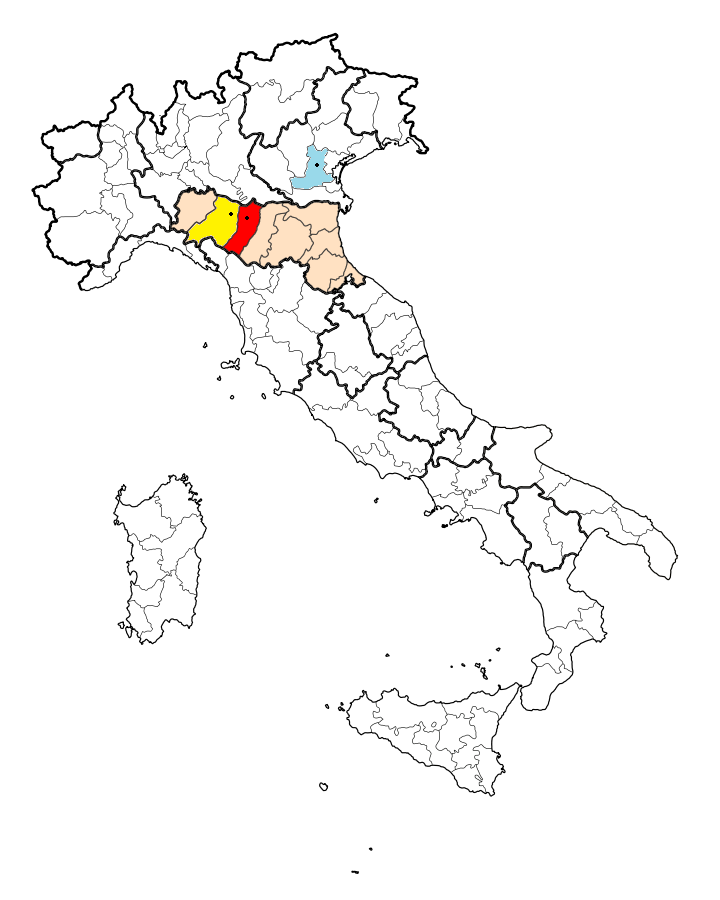
\includegraphics[height=1.0\textheight]{include/3-cities-map.png}
%\caption{{Location of the city of Parma, Reggio Emilia, and Padova, Italy.}}
\end{figure}
\end{center}
\end{frame}
%%%-----------------------------------------------------------------------------------------------
%\begin{frame}
%\frametitle{Definition of treatment variable}\label{frame:treatment}
%Type of infant-toddler center and preschool attended inferred from:
%\begin{itemize}
%	\item Both name and address \hyperlink{fig:ReggioSchools}{\beamerbutton{map}}
%	\item Self-reported type
%	\vspace{2ex}
%	\item Caregiver report for child and ado
%	\item Self-report for adults
%\end{itemize}
%
%\vspace{1ex}
%
%$\Rightarrow$ potential for measurement error in recall
%\end{frame}
%\subsection{Sample}\label{sec:sample}
%-----------------------------------------------------------------------------------------------
\begin{frame}
\frametitle{Sampling Design}\label{frame:design}
\begin{itemize}
	\item Stratified by \textbf{cohort}, key periods in the lifecycle:
	\begin{itemize}
		\usebeamerfont{smalltable}
		\item age 6 (children entering elementary school);
		\item age 17 (adolescents reaching maturity);
		\item age 31-32 (adults at first life milestone);
		\item age 40-41 (adults at second life milestone; first to have access to infant-todder centers);
		\item age 53-58 (adults born before the Reggio Children Approach was implemented).
	\end{itemize}
	\item Sampling frame taken from population registries (anagrafi)
	\item Random sample households resident in the city since birth. \hyperlink{frame:TotRefSample}{\beamergotobutton{}}
	\item Screen households to oversample treatment group.
	%\item A minimum sample size of 150 treated and 150 controls for each stratum has been reached.
	\item Harmonized questionnaire: background info, health, cognitive, socio-emotional, trust, etc.
	\item Professional data collection agency.
\end{itemize}
\end{frame} 

%%---------------------------------------------------------------------------------------------------------------------------------
%\begin{frame}\label{frame:TotRefSample}
%\begin{table}[ht!]
\caption{\textbf{\small Total Reference Sample}}
\label{tab:TotRefSample}
%%\vspace{-5mm}
\begin{center}
\scriptsize
\begin{tabular}{ l c c c c }
\hline\hline
\textbf{Cohort} & \textbf{Reggio} & \textbf{Parma} & \textbf{Padova} & \textbf{Total}\\
\hline
Italian Children born in 2006 (Cohort V)   & 1,096 & 1,054 & 1,224 & 3,374\\[0.2em]
Immigrant Children born in 2006 (Cohort V) &   296 &   224 &   264 &   784\\[0.2em]
Adolescents born in 1994 (Cohort IV)       &   865 &   806 & 1,113 & 2,784\\[0.2em]
Adults born in 1980-81 (Cohort III)        & 1,205 & 1,355 & 1,630 & 4,190\\[0.2em]
Adults born in 1969-70 (Cohort II)         & 1,655 & 2,057 & 2,200 & 5,912\\[0.2em]
Adults born in 1954-59 (Cohort I)          & 3,646 & 3,999 & 5,587 & 13,232\\[0.2em]
\hline
Total                                      & 8,763 & 9,495 & 12,018 & 30,276\\
\hline
\end{tabular}
\end{center}
\begin{flushleft}
\tiny{{\bfseries Notes:} Total number of names provided by the population registries who satisfied the selection criteria (born in the city of residence and of Italian citizenship -- except for Immigrant Children born in 2006), broken down by City and Cohort. Source: authors calculations on data provided by the population registries.}
\end{flushleft}
\end{table} 
%%\hyperlink{frame:design}{\beamergotobutton{back}}
%\end{frame}
%%---------------------------------------------------------------------------------------------------------------------------------
%\begin{frame}\label{frame:SameCity}
%\begin{table}[ht!]
\caption{\textbf{Percentage of people living in the same city since birth, by cohort}}
\label{tab:SameCity}
\vspace{-5mm}
\begin{center}
\begin{tabular}{ l c c c c }
\hline\hline
\textbf{Cohort} & \textbf{Reggio (\%)} & \textbf{Parma (\%)} & \textbf{Padova (\%)} & \textbf{Total (\%)}\\
\hline
Italian Children born in 2006 (Cohort V)   & 61.3  & 70.2  & 65.1  & 65.2 \\[0.2em]
Adolescents born in 1994 (Cohort IV)       & 58.1  & 63.0  & 64.4  & 61.9 \\[0.2em]
Adults born in 1980-81 (Cohort III)        & 26.5  & 27.5  & 32.6  & 29.0 \\[0.2em]
Adults born in 1969-70 (Cohort II)         & 27.9  & 31.6  & 31.9  & 30.6 \\[0.2em]
Adults born in 1954-59 (Cohort I)          & 28.8  & 27.9  & 31.4  & 29.5 \\[0.2em]
\hline
\textit{Total}         & \textit{32.3\%}  & \textit{32.5\%}  & \textit{35.2\%} & \textit{33.5\%} \\
\hline
\end{tabular}
\end{center}
\footnotesize{{\bfseries Notes:} Reference sample who satisfied the selection criteria (born in the city of residence and of Italian citizenship) as a percentage of the total number of names given by the population registries, broken down by City and Cohort. Source: authors calculations on data provided by the population registries.}
\end{table}

%%\hyperlink{frame:design}{\beamergotobutton{back}}
%\end{frame}
%%-----------------------------------------------------------------------------------------------
\begin{frame}
\frametitle{Attendance Infant-toddler Centers (0-3)} 
\begin{center}
\begin{figure}
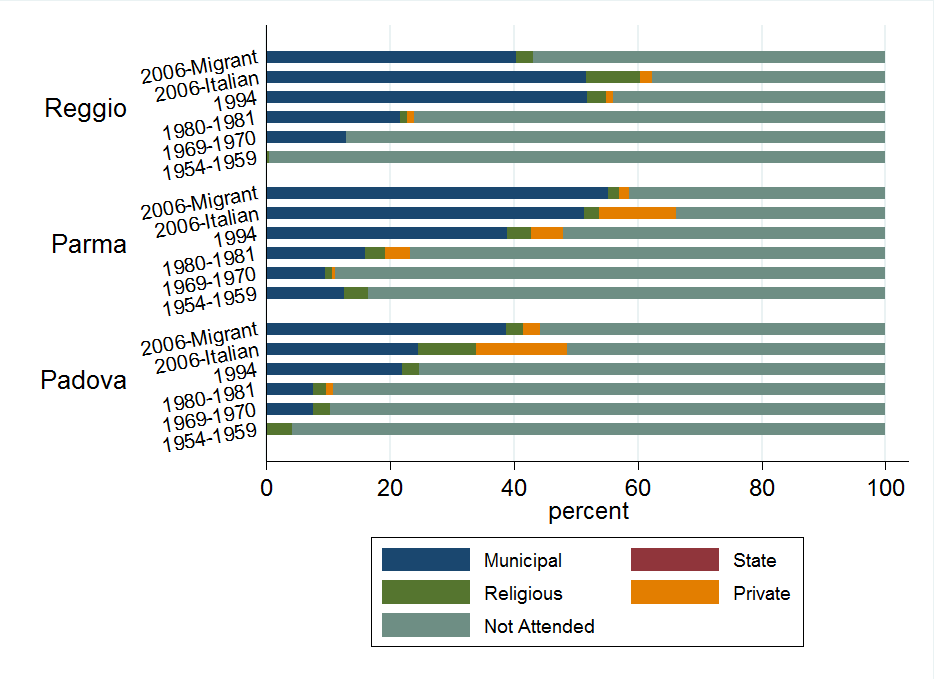
\includegraphics[width=1.15\textheight]{include/asiloType-Attend.png}
%\caption{{Location of the city of Parma, Reggio Emilia, and Padova, Italy.}}
\end{figure}
\end{center}
\end{frame}
%%-----------------------------------------------------------------------------------------------
\begin{frame}
\frametitle{Attendance Preschools (3-6)} 
\begin{center}
\begin{figure}
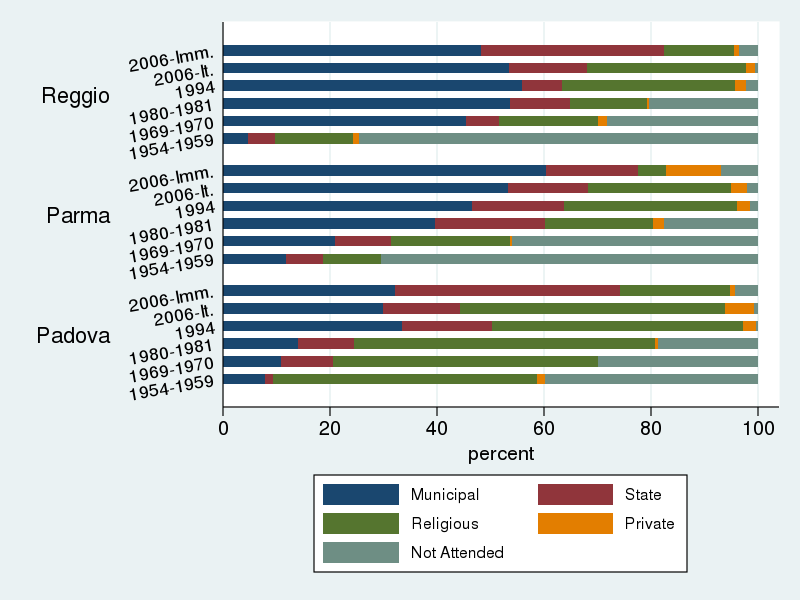
\includegraphics[width=1.15\textheight]{include/maternaType-Attend.png}
%\caption{{Location of the city of Parma, Reggio Emilia, and Padova, Italy.}}
\end{figure}
\end{center}
\end{frame}
%%%-----------------------------------------------------------------------------------------------
%\begin{frame}
%\frametitle{Questionnaire Design}
%Develop a \textbf{harmonized questionnaire} for Reggio Emilia and the two comparison cities.
%\begin{itemize}
%\item Household Background information (family characteristics, SES).
%	\begin{itemize}
%		\item family composition, gender, origin, education, profession
%	\end{itemize}
%\item Child-care choices
%\item Motives and experience of child care use (for the parents).
%\item Several outcomes: health, socio-emotional skills skills, social capital, trust, attitudes towards migration
%%\item \underline{Health capital}: height, weight, physical and mental health, healthy behavior, eating and sleeping habits.
%%\item \underline{Social capital}: voluntary and charity work, provision of care, type of care provided, participation in clubs and organizations.
%%\item \underline{Friendship}: number and gender composition of friends, duration and strength of friendship ties, frequency and type of contacts.
%%\item Development of trust/reciprocity.
%%\item Parenting styles (older cohorts).
%%\item Attitudes towards immigration (special module on immigration).
%\end{itemize}
%
%\vspace{2ex}
%
%Currently focusing on socio-emotional skills: main objective of the education approach
%
%\end{frame} 

\subsection{Baseline Characteristics}\label{sec:baseline}

\begin{frame}
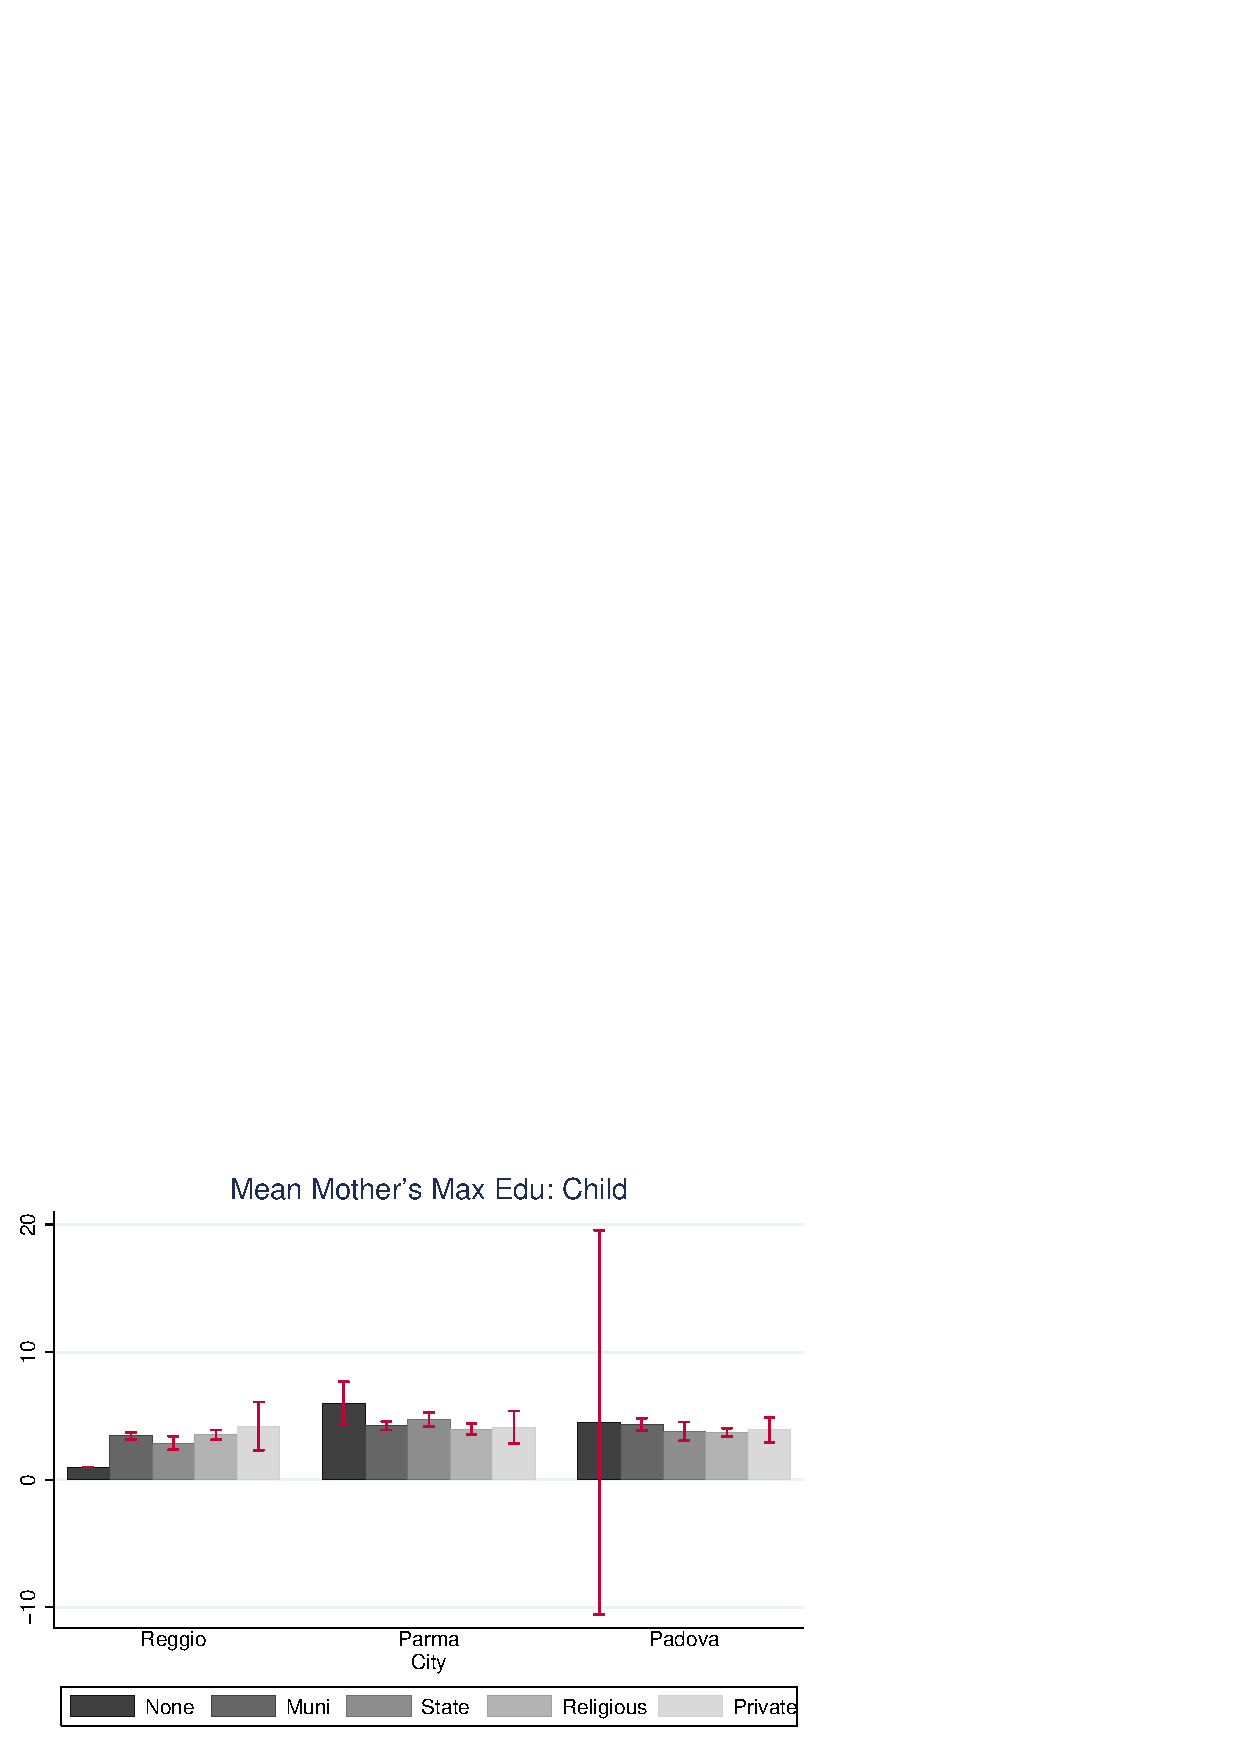
\includegraphics[scale = 0.85]{../../Output/graphs/baseline/baseline_momMaxEdu_Child.pdf}
\end{frame}

\begin{frame}
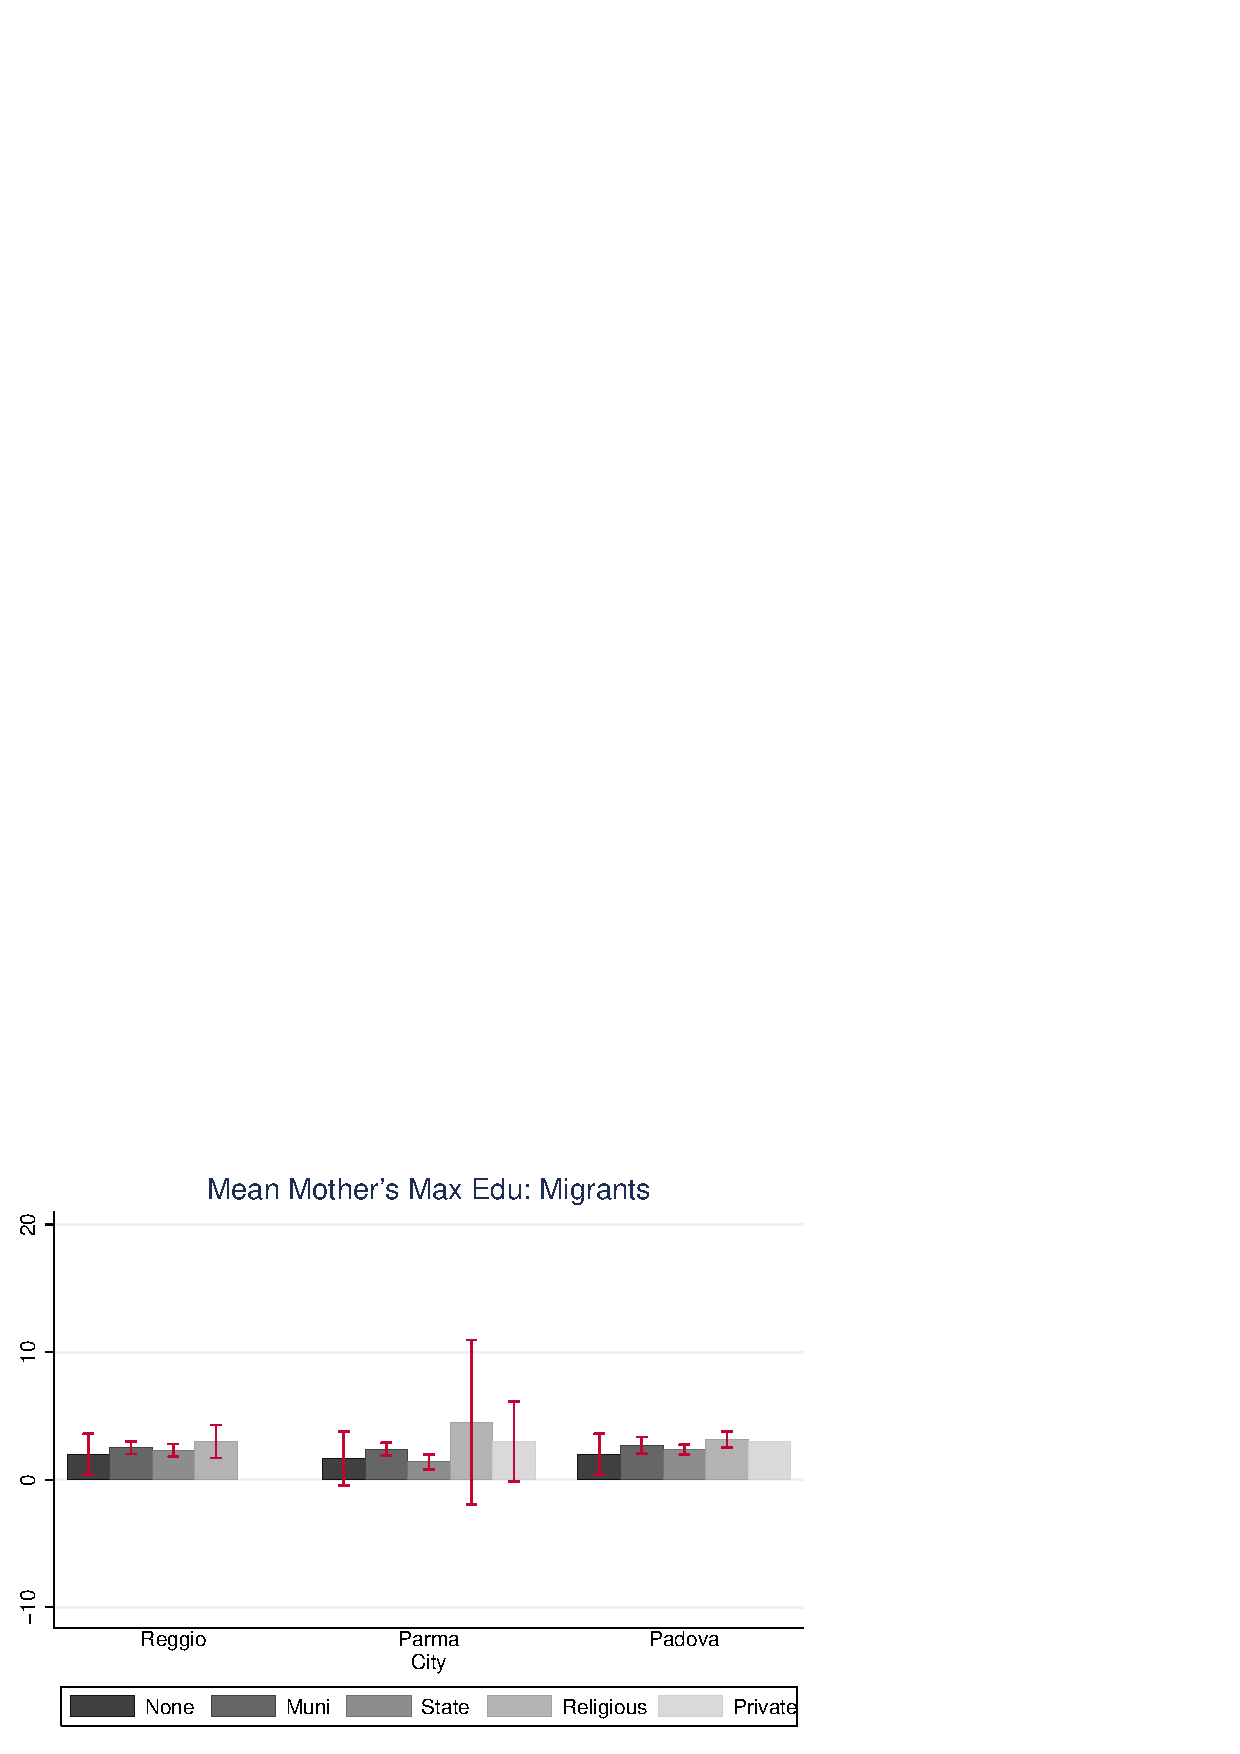
\includegraphics[scale = 0.85]{../../Output/graphs/baseline/baseline_momMaxEdu_Migrants.pdf}
\end{frame}

\begin{frame}
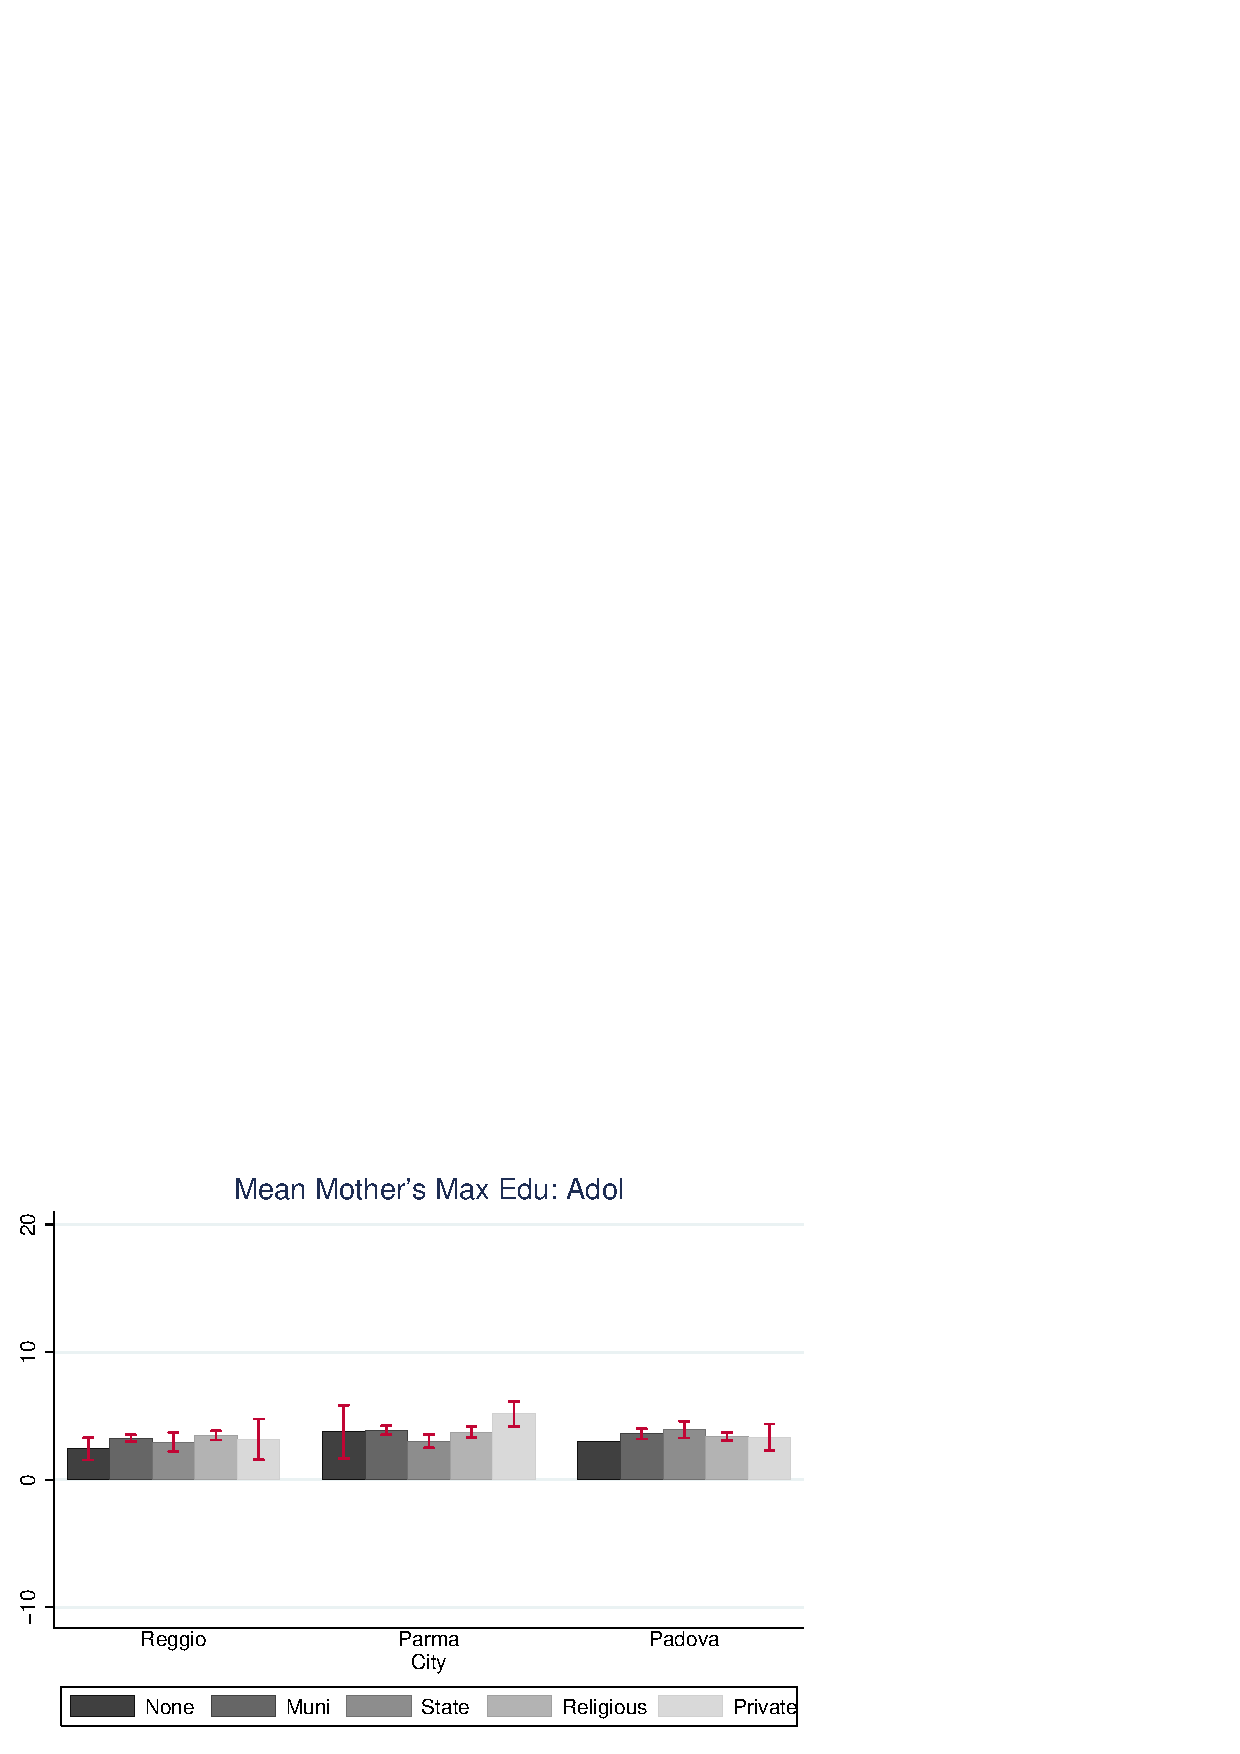
\includegraphics[scale = 0.85]{../../Output/graphs/baseline/baseline_momMaxEdu_Adol.pdf}
\end{frame}

\begin{frame}
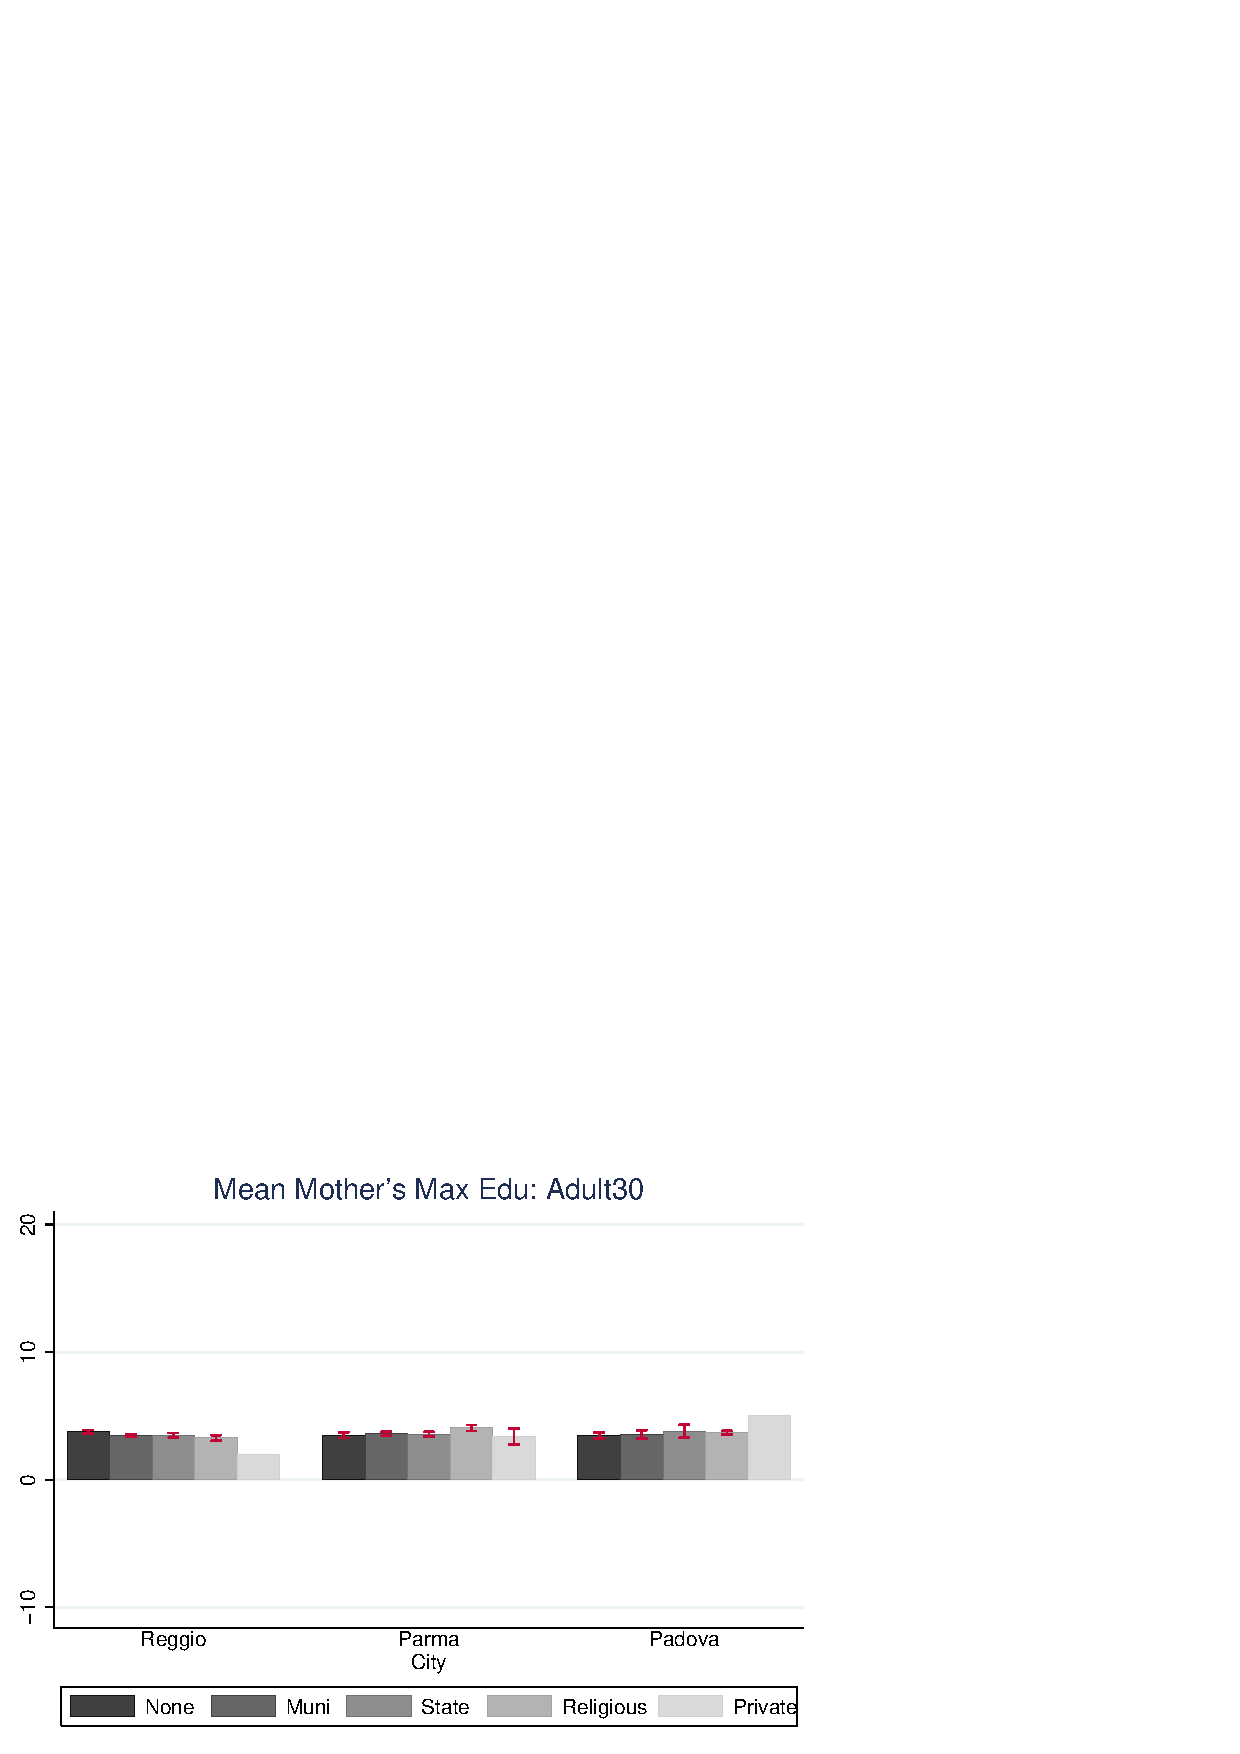
\includegraphics[scale = 0.85]{../../Output/graphs/baseline/baseline_momMaxEdu_Adult30.pdf}
\end{frame}

\begin{frame}
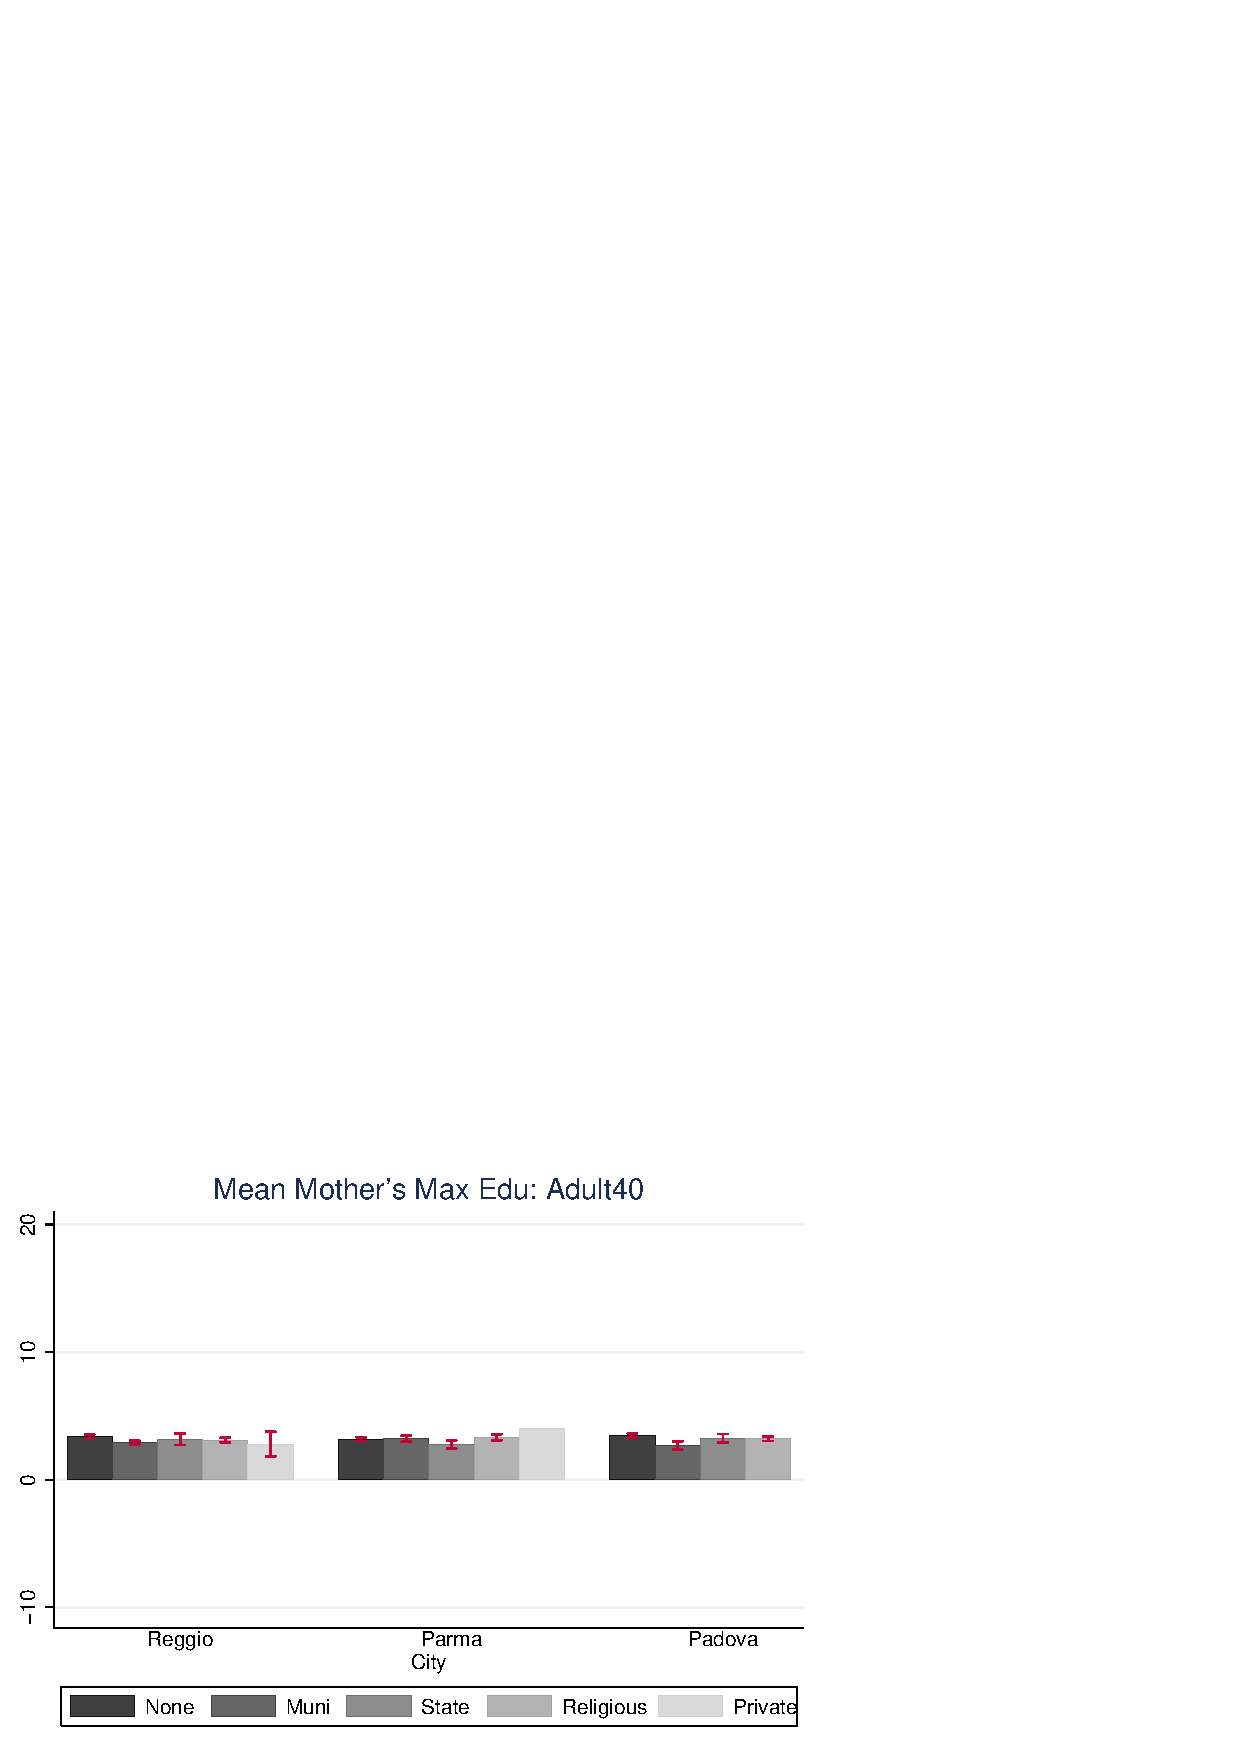
\includegraphics[scale = 0.85]{../../Output/graphs/baseline/baseline_momMaxEdu_Adult40.pdf}
\end{frame}

\begin{frame}
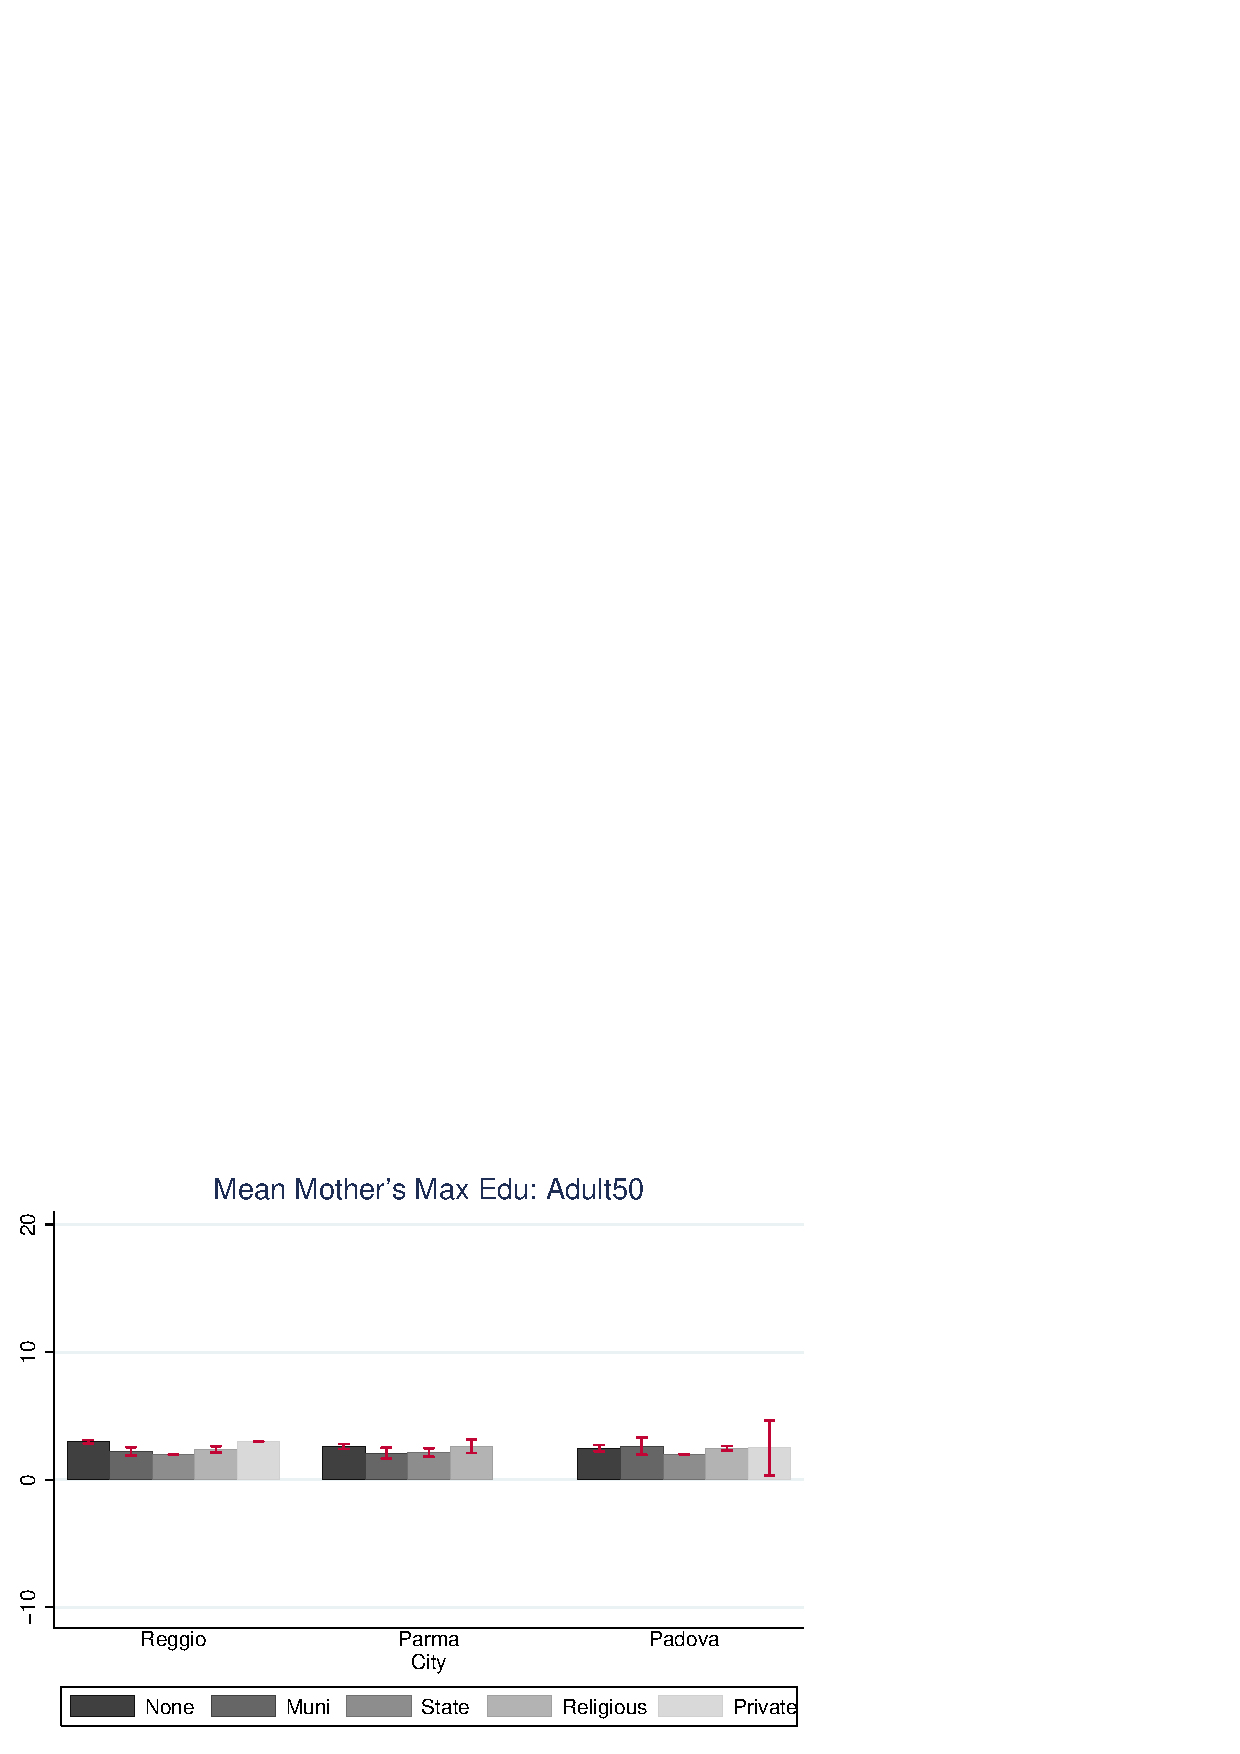
\includegraphics[scale = 0.85]{../../Output/graphs/baseline/baseline_momMaxEdu_Adult50.pdf}
\end{frame}

\begin{frame}
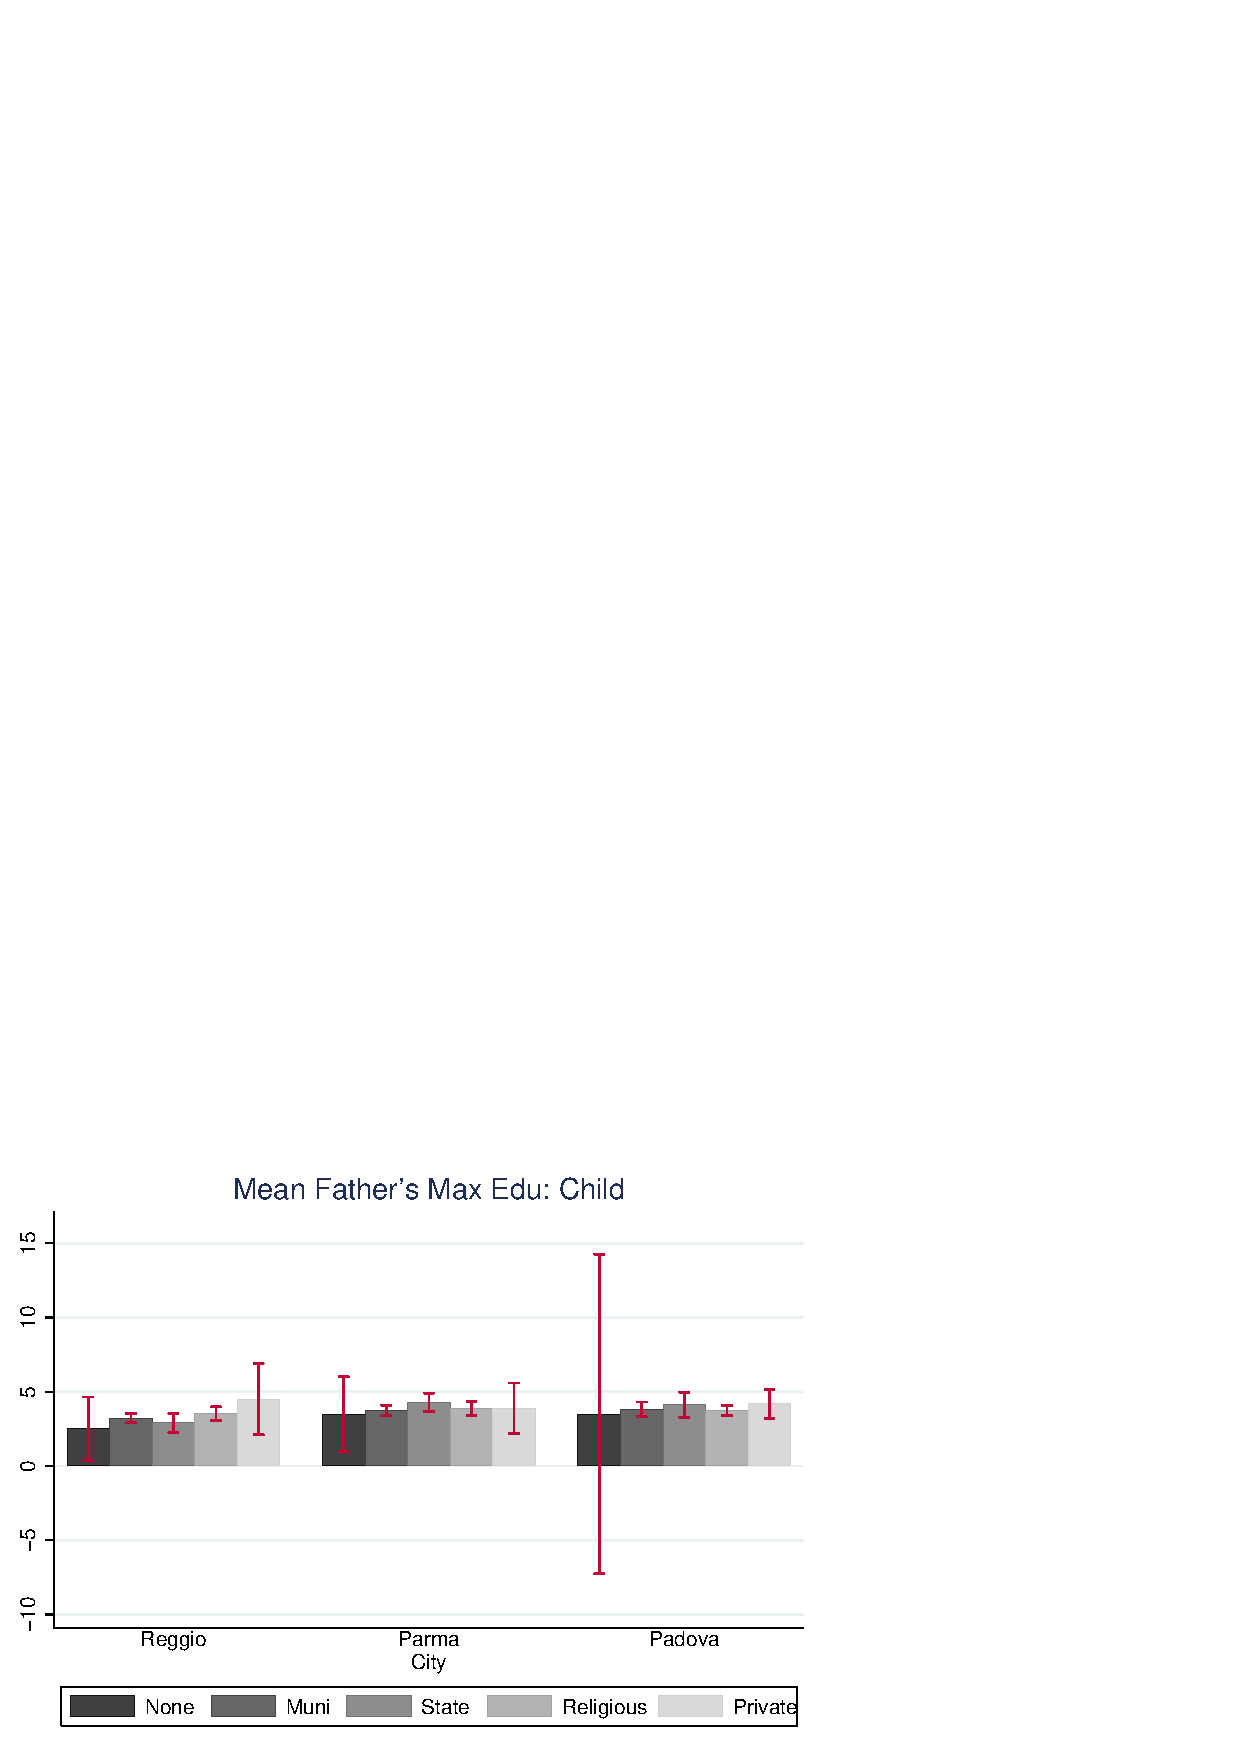
\includegraphics[scale = 0.85]{../../Output/graphs/baseline/baseline_dadMaxEdu_Child.pdf}
\end{frame}

\begin{frame}
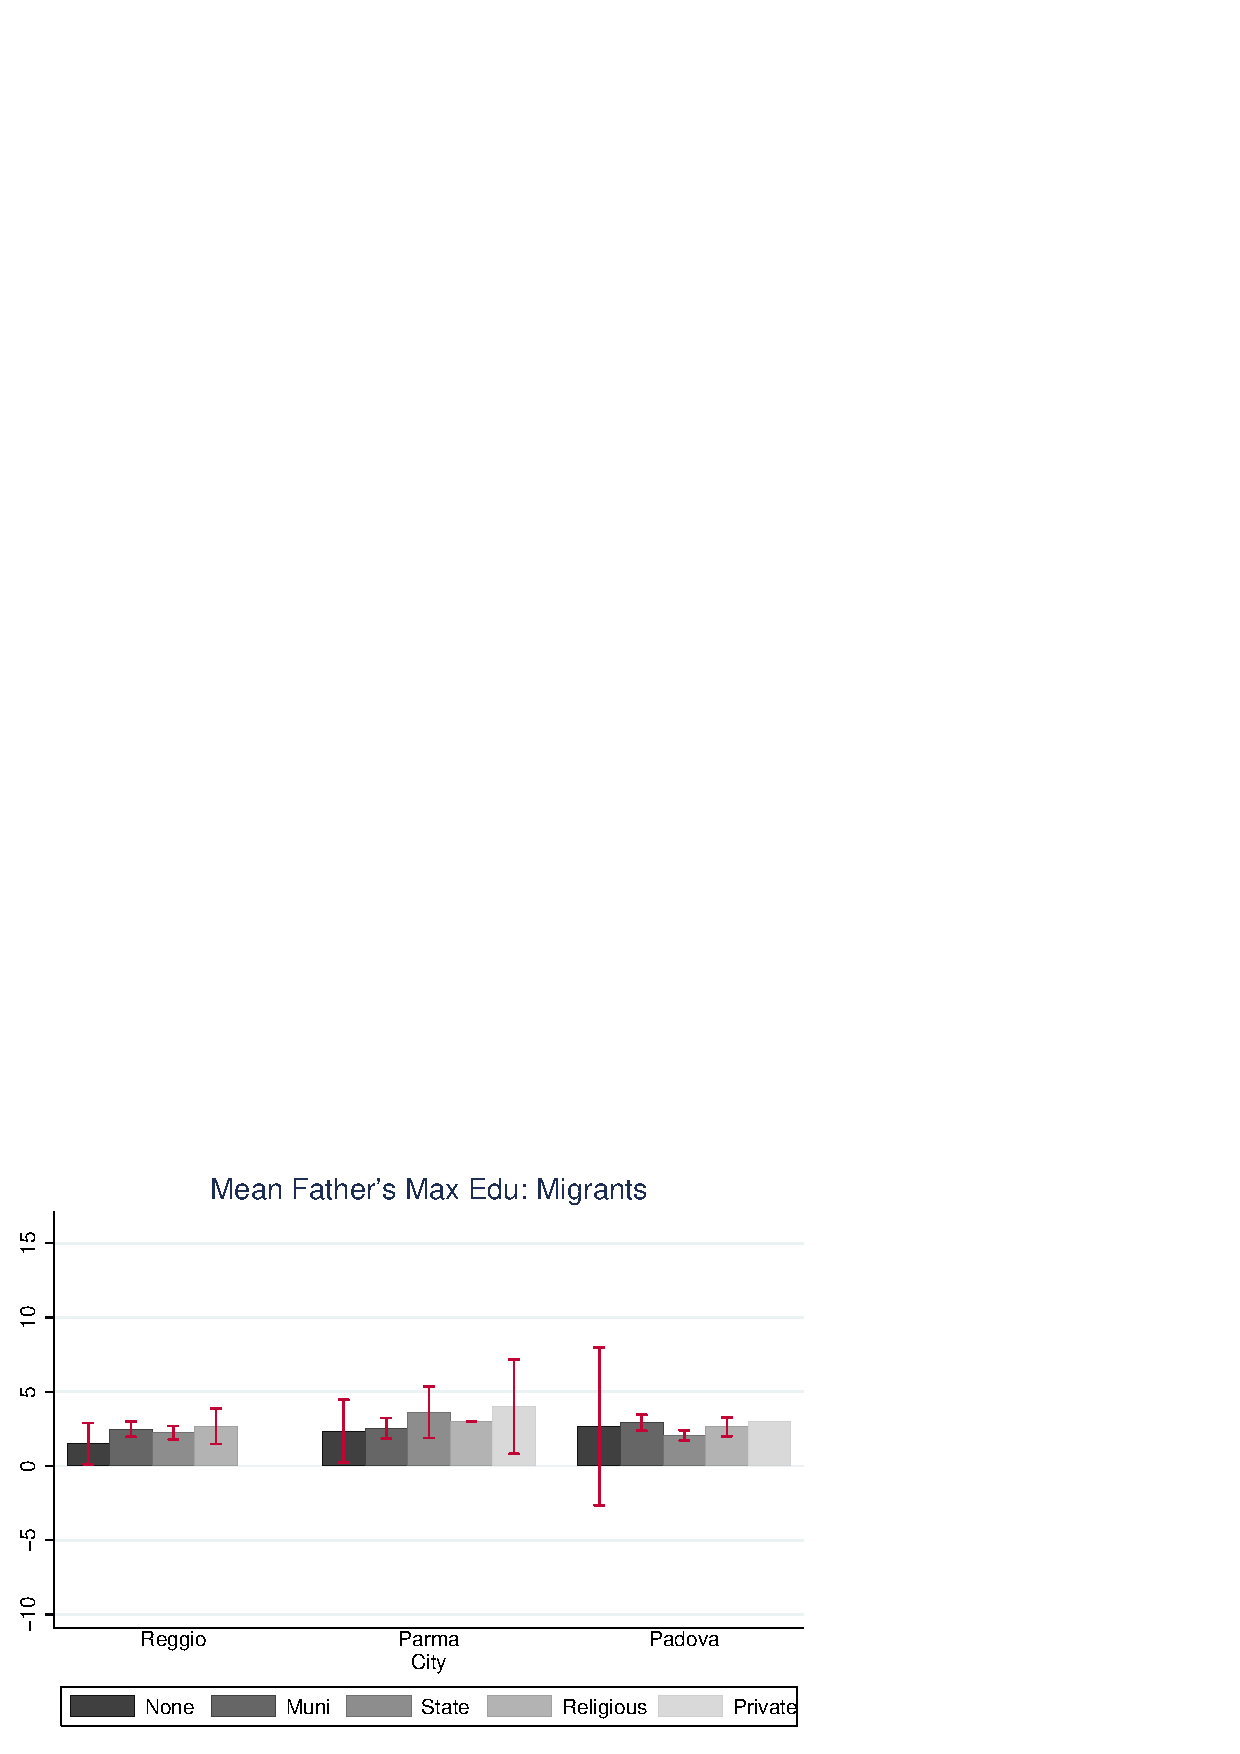
\includegraphics[scale = 0.85]{../../Output/graphs/baseline/baseline_dadMaxEdu_Migrants.pdf}
\end{frame}

\begin{frame}
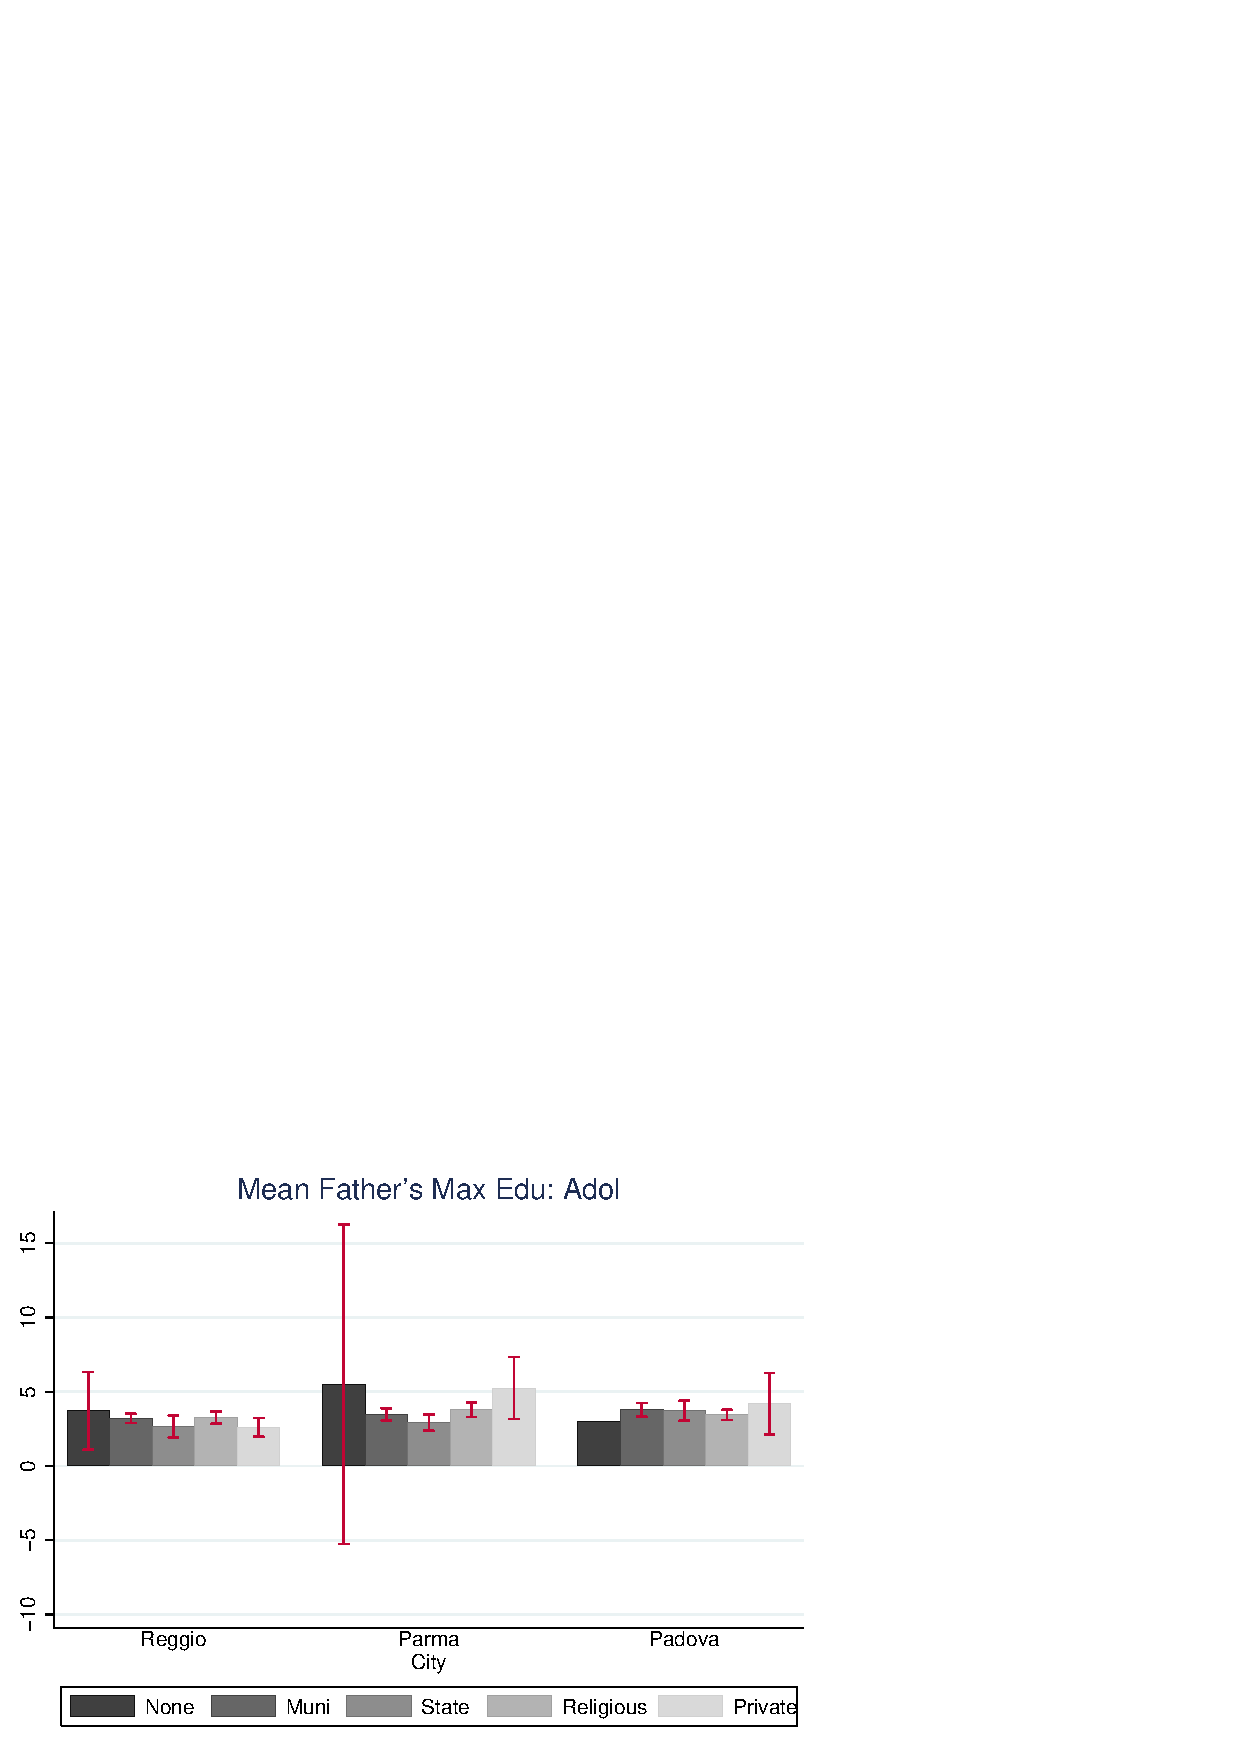
\includegraphics[scale = 0.85]{../../Output/graphs/baseline/baseline_dadMaxEdu_Adol.pdf}
\end{frame}

\begin{frame}
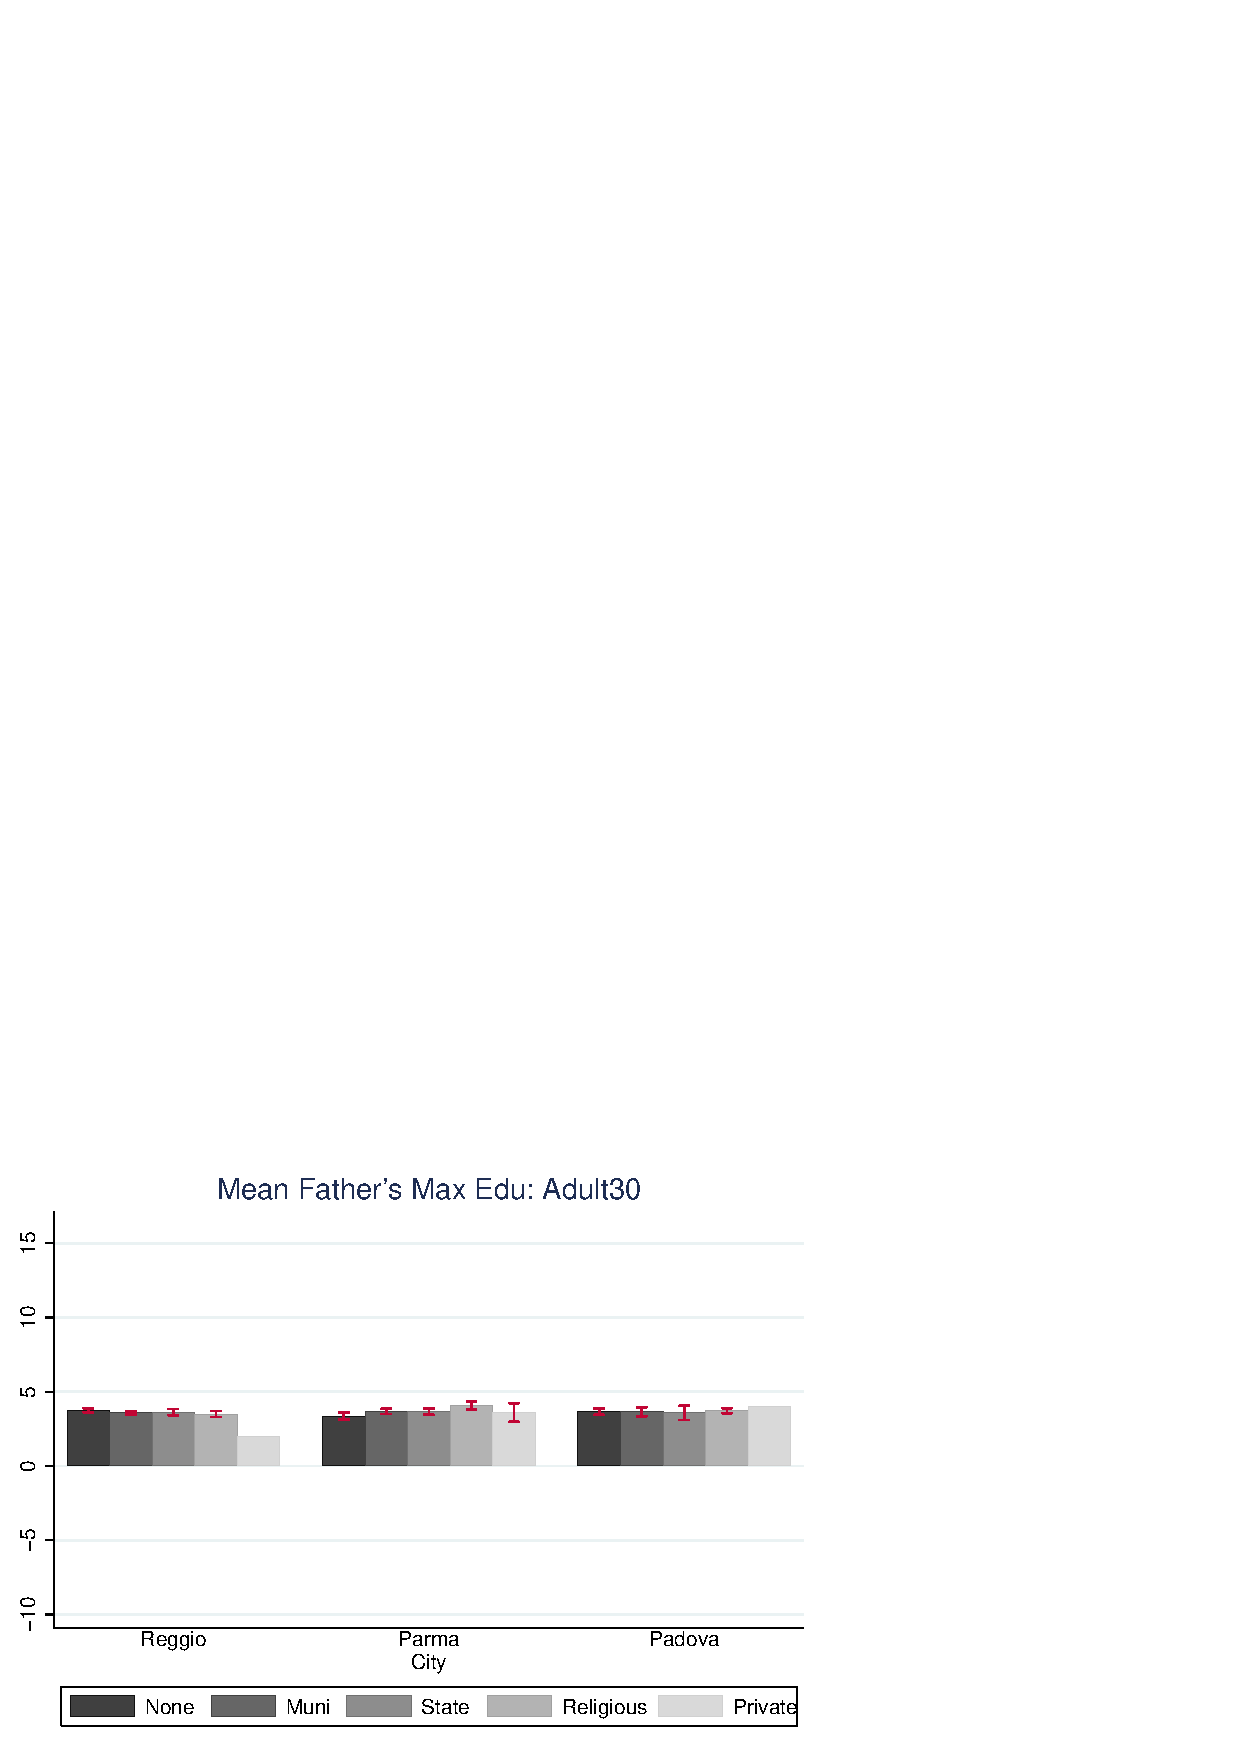
\includegraphics[scale = 0.85]{../../Output/graphs/baseline/baseline_dadMaxEdu_Adult30.pdf}
\end{frame}

\begin{frame}
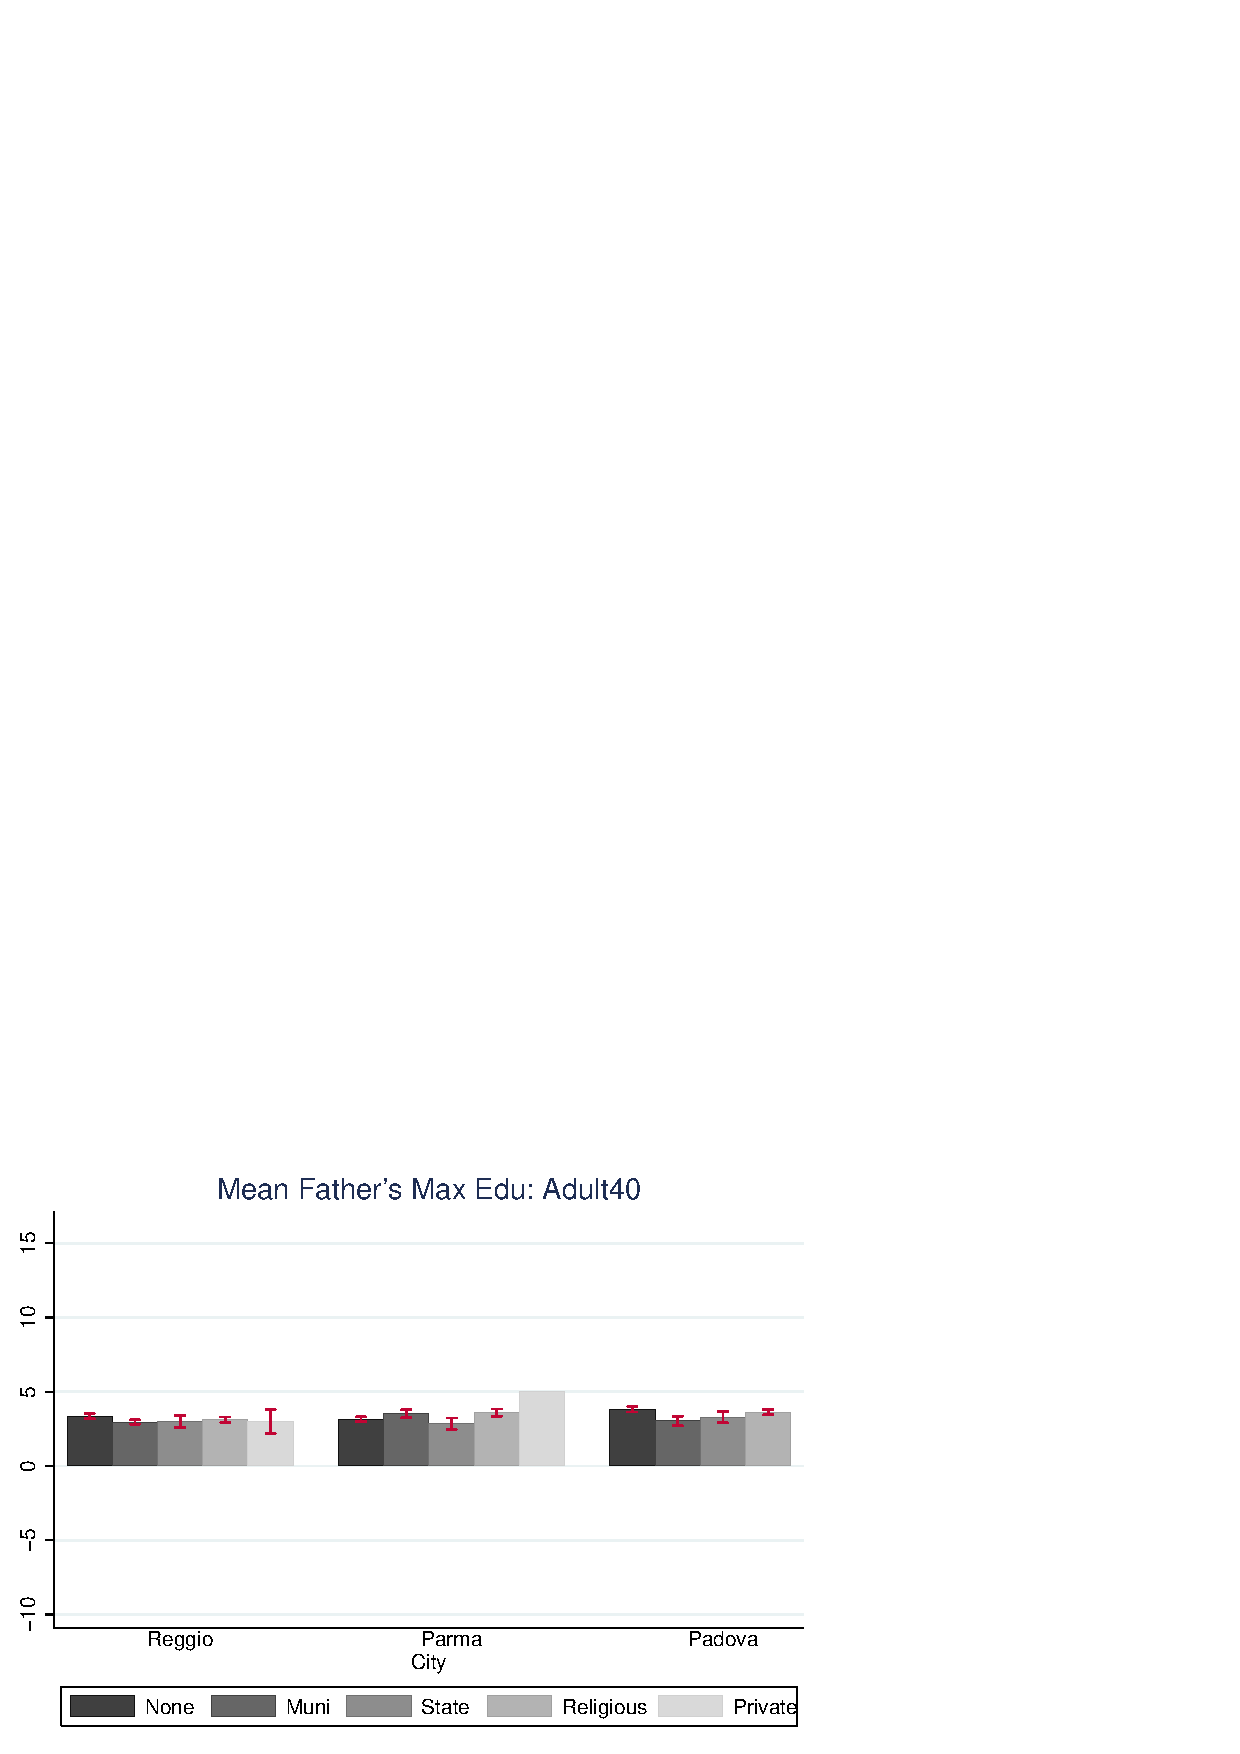
\includegraphics[scale = 0.85]{../../Output/graphs/baseline/baseline_dadMaxEdu_Adult40.pdf}
\end{frame}

\begin{frame}
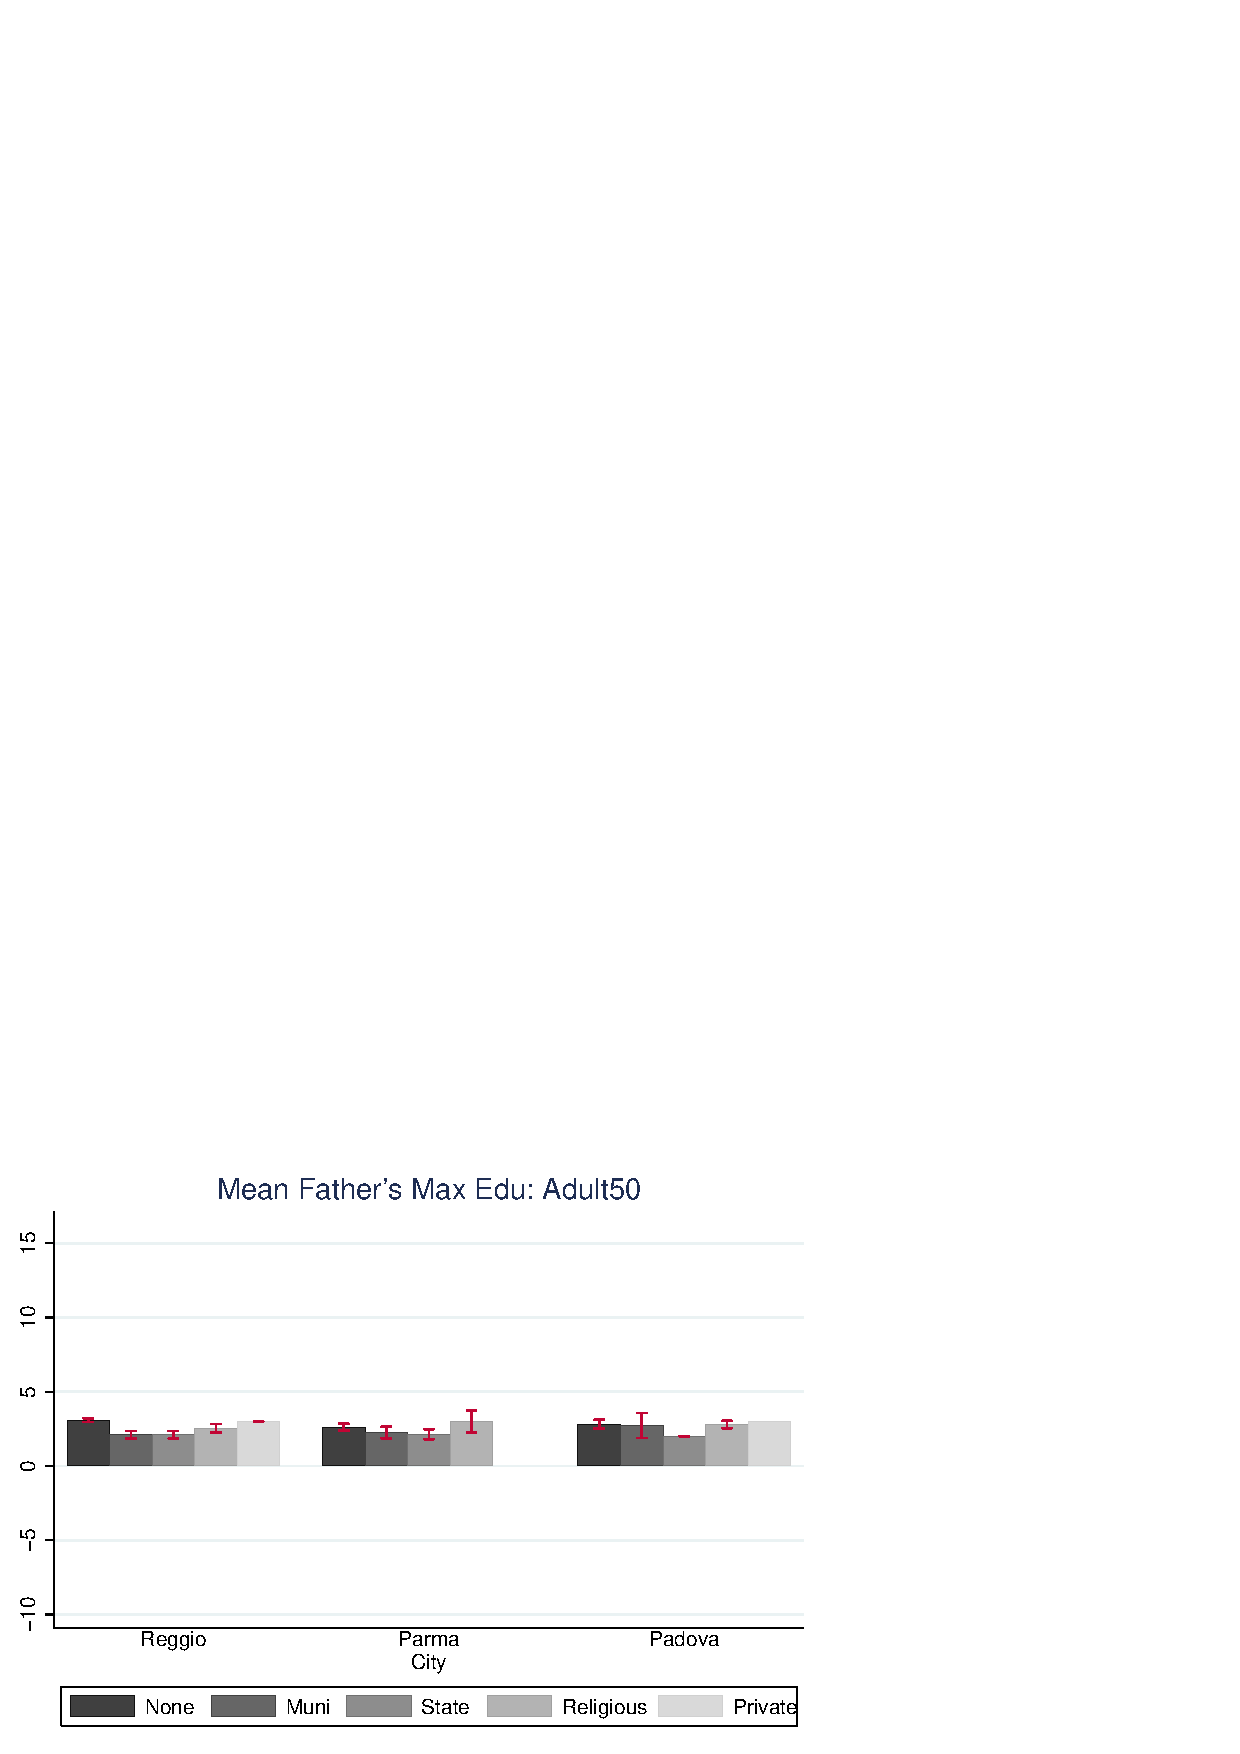
\includegraphics[scale = 0.85]{../../Output/graphs/baseline/baseline_dadMaxEdu_Adult50.pdf}
\end{frame}

\begin{frame}
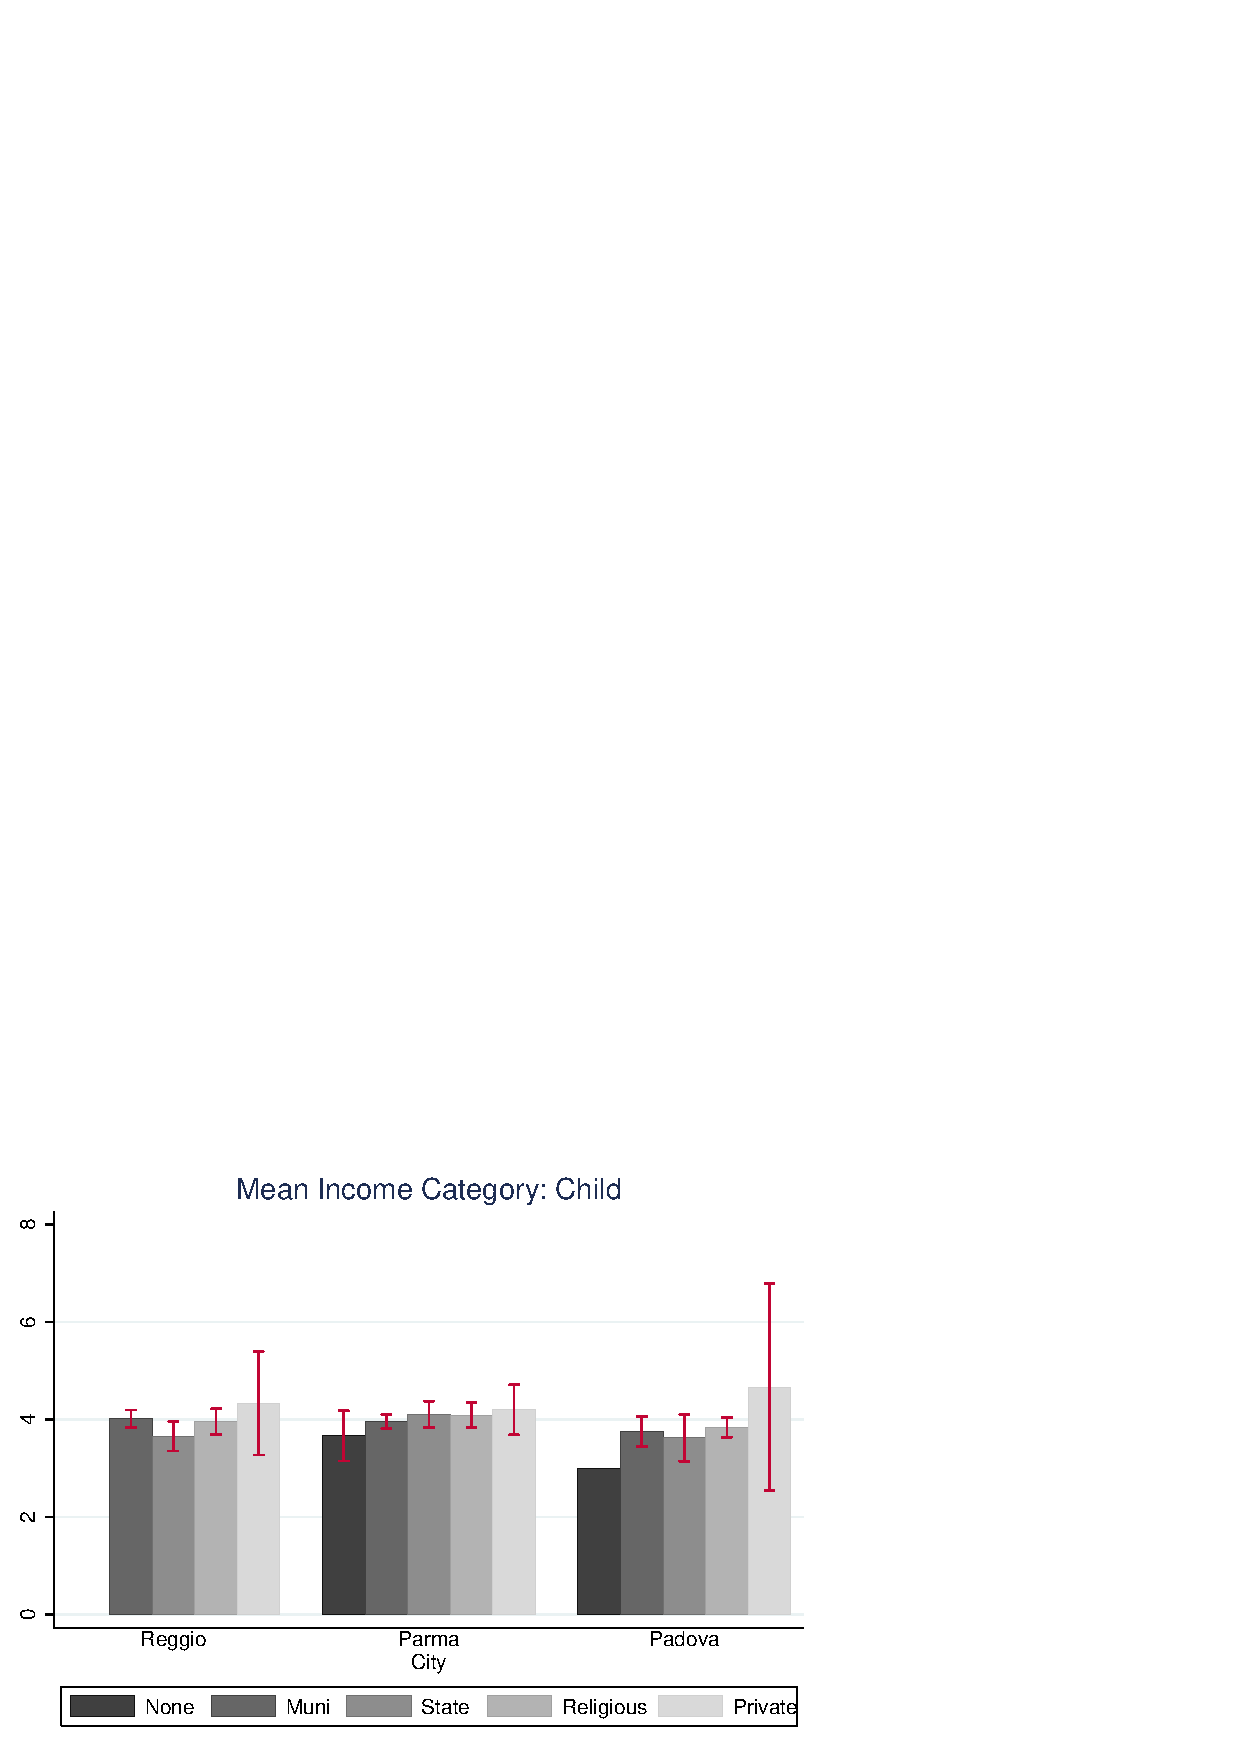
\includegraphics[scale = 0.85]{../../Output/graphs/baseline/baseline_cgIncomeCat_Child.pdf}
\end{frame}

\begin{frame}
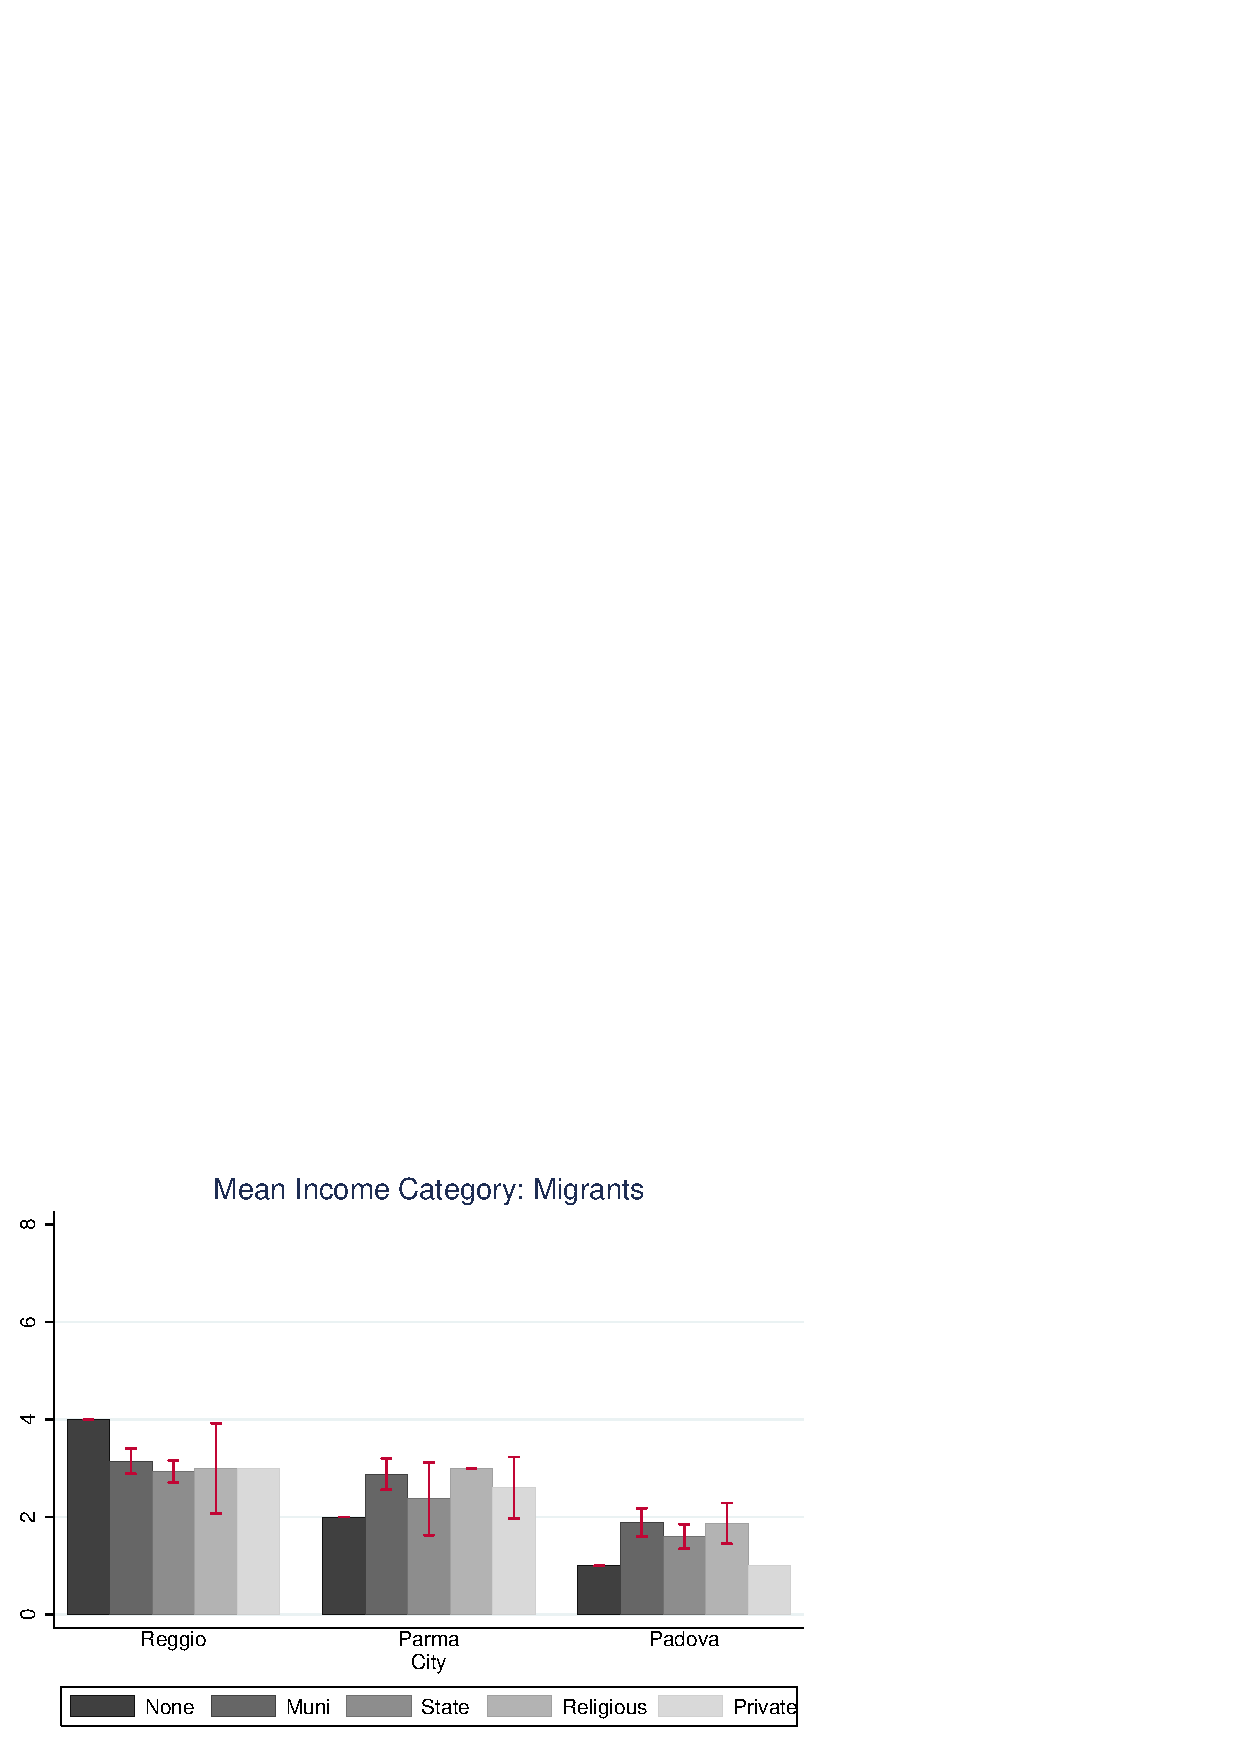
\includegraphics[scale = 0.85]{../../Output/graphs/baseline/baseline_cgIncomeCat_Migrants.pdf}
\end{frame}

\begin{frame}
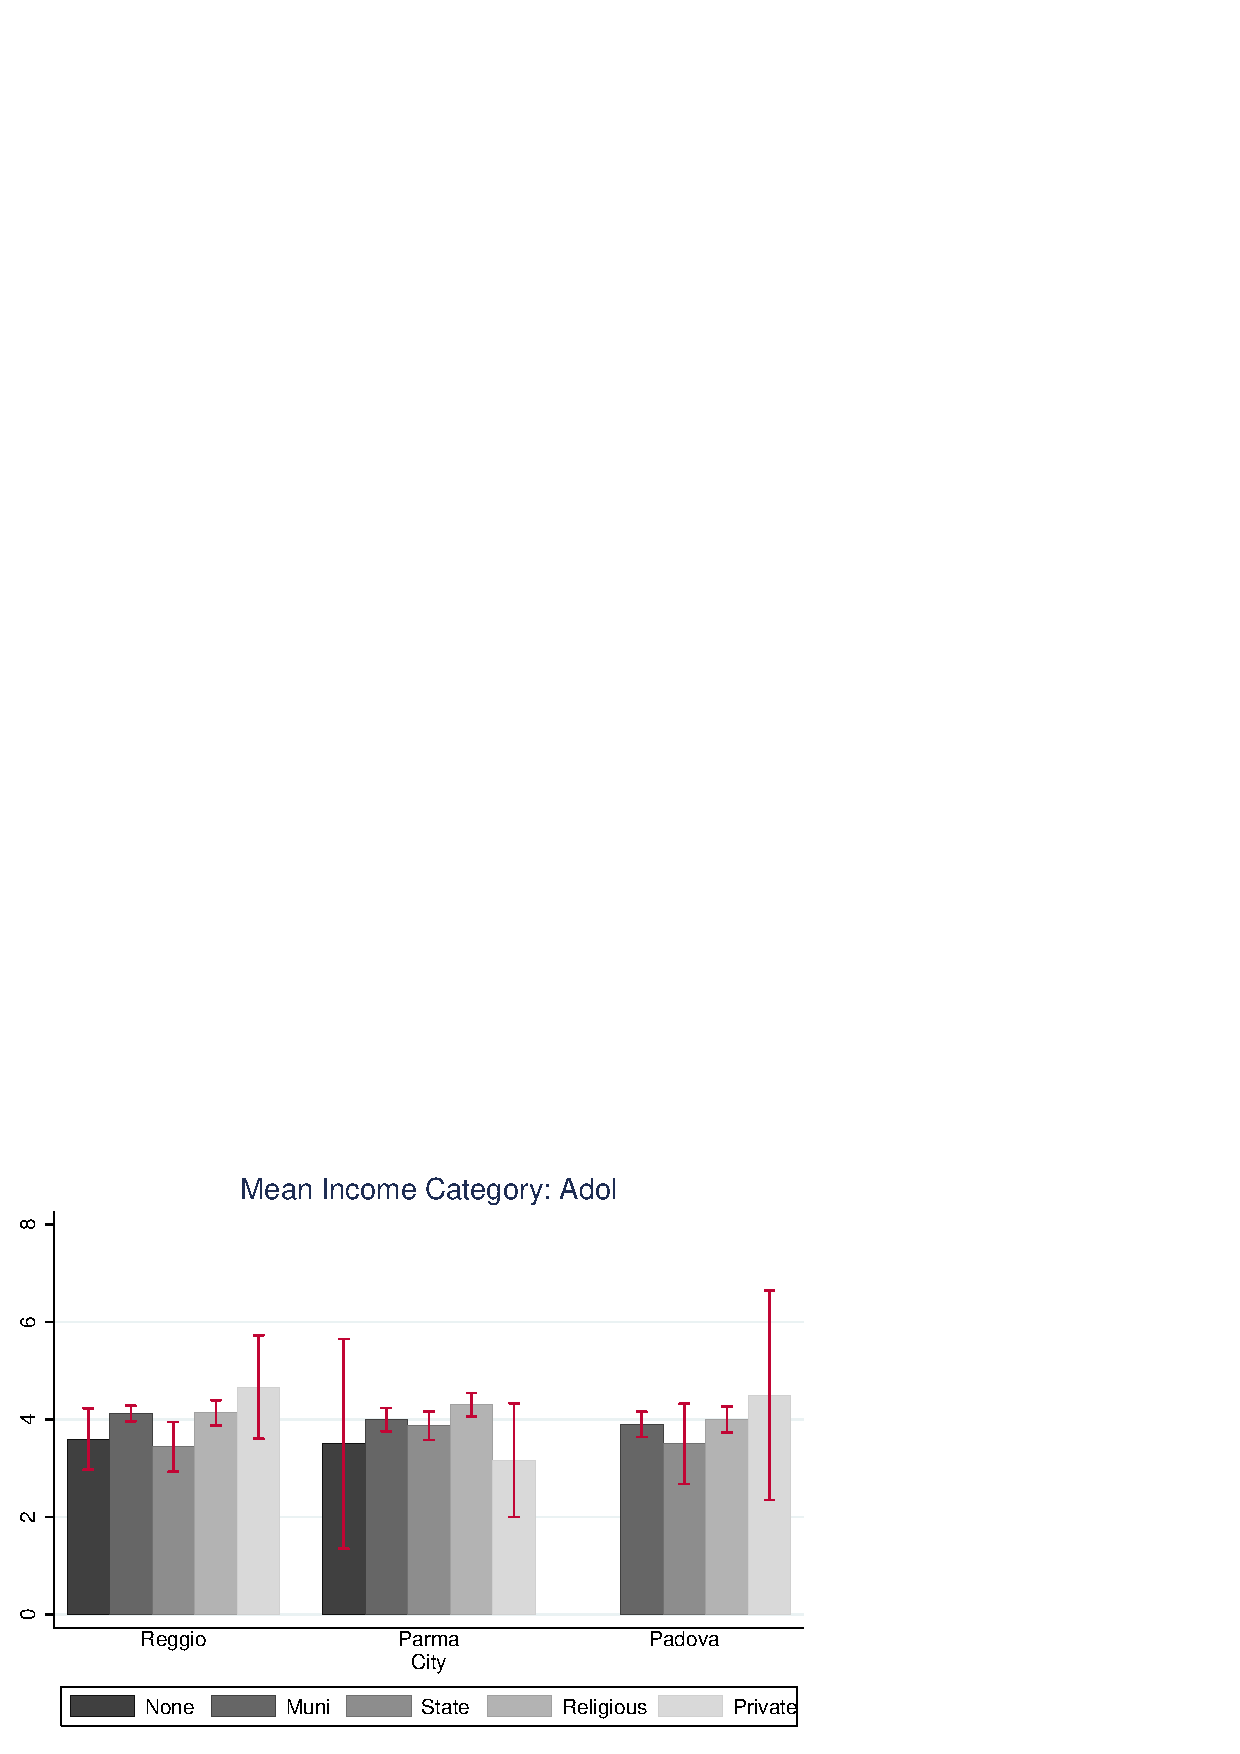
\includegraphics[scale = 0.85]{../../Output/graphs/baseline/baseline_cgIncomeCat_Adol.pdf}
\end{frame}



\subsection{Strategy}\label{sec:strategy}
%%-----------------------------------------------------------------------------------------------
\begin{frame} \frametitle{Specification 1: OLS Without Controls}
%Pooling all three cities, and running the model separately for infant-toddler centers (age 0-3) and preschools (age 3-6), we 
Consider the simplest specification:
\begin{align*} \label{OLS-nocontrol}
	y_{i} & = \gamma_0 + \gamma_1 s_{i,2} + \gamma_2 s_{i,3} + \gamma_3 s_{i,4} +\varepsilon_{i}, \\
	 i \in I & := \{ \text{individuals in city $j$ and age cohort $h$}\}
\end{align*}
\begin{itemize}
\item $\mathbf{y_{i}}$: Outcome of interest for individual $i$
\item $\mathbf{s_{i,k}}$: Type of materna school (2: No preschool, 3: State Preschool, 4: Religious Preschool)
\end{itemize}

\end{frame}


%-----------------------------------------------------------------------------------------------
\begin{frame} \frametitle{Specification 2: OLS With Controls}
%Pooling all three cities, and running the model separately for infant-toddler centers (age 0-3) and preschools (age 3-6), we 
Consider the specification:
\begin{align*}
	y_{i} & = \gamma_0 + \gamma_1 s_{i,2} + \gamma_2 s_{i,3} + \gamma_3 s_{i,4} + \mathbf{X}\beta +\varepsilon_{i}, \\
	 i \in I & := \{ \text{individuals in city $j$ and age cohort $h$}\}
\end{align*}
\begin{itemize}
\item $\mathbf{y_{i}}$: Outcome of interest for individual $i$
\item $\mathbf{s_{i,k}}$: Type of materna school (2: No preschool, 3: State Preschool, 4: Religious Preschool)
\item $\mathbf{X}$: A vector of baseline variables that have the lowest BIC score.
\end{itemize}

\end{frame}




%-----------------------------------------------------------------------------------------------
\begin{frame} \frametitle{Specification 3: Diff-in-diff With Controls}

We consider two routes of analysis with the difference-in-difference approach.
\begin{enumerate}
\item \textbf{Fix city:} estimate the differences in outcomes across cohorts for different choices in preschool types in each city
\item \textbf{Fix age cohort:} estimate the differences in outcomes across cities for different choices in preschool types in each age cohort
\end{enumerate}

\end{frame}


%-----------------------------------------------------------------------------------------------
\begin{frame} \frametitle{Diff-in-diff Example: Fixing City}

Let's consider a case with 
\begin{itemize}
\item 3 adult cohorts, denoted by the number in subscript of $k$
\item 4 school types, denoted by the number in subscript for $s$ \\\ 
\end{itemize}


Assuming that we restrict our sample to people in Reggio, we can write our model for a certain outcome $y$ as:
\begin{eqnarray}  \label{eq:specific2}
y_i & = & \gamma_0 + \gamma_1 k_{i,2} + \gamma_2 k_{i,3} + \gamma_3 s_{i,2} + \gamma_4 s_{i,3} + \gamma_5 s_{i,4} + \gamma_6 ({k_{i,2}}\cdot{s_{i,2}}) 
\nonumber \\ 
& + & \gamma_7 ({k_{i,2}}\cdot{s_{i,3}}) + \gamma_8 ({k_{i,2}}\cdot{s_{i,4}}) + \gamma_9 ({k_{i,3}}\cdot{s_{i,2}}) + \gamma_{10} ({k_{i,3}}\cdot{s_{i,3}})  \nonumber \\ 
& + &\gamma_{11} ({k_{i,3}}\cdot{s_{i,4}}) + \mathbf{X}\beta + \varepsilon_i  
\end{eqnarray}

\end{frame}


%-----------------------------------------------------------------------------------------------
\begin{frame} \frametitle{Interpreting the Simple Difference}

Assume two cases
\begin{enumerate}
\item A Reggio individual in Age 50 cohort and did not attend any preschool
\item A Reggio individual in Age 50 cohort and attended municipal school
\end{enumerate}
\begin{eqnarray*}  
    \mathbb{E}[y \mid k_1 = 1, s_1 = 1] & = & \gamma_0 + \mathbf{X}\beta  \\
    \mathbb{E}[y \mid k_1 = 1, s_2 = 1] & = & \gamma_0 + \gamma_1 + \mathbf{X}\beta      
\end{eqnarray*}

$\gamma_1$ is interpreted as ``the mean difference in outcome between the group (2) and group (1)." \\\

Although this estimator can be informative, the treatment effect can be confounded due to \underline{the permanent average differences} in baseline characteristics between people who choose to go to different types of preschool.

\end{frame}


%-----------------------------------------------------------------------------------------------
\begin{frame} \frametitle{Interpreting the Diff-in-Diff}
\begin{footnotesize}
Assume four cases: 
\begin{enumerate}
\item A Reggio individual lives in 50's and did not attend preschool
\item A Reggio individual lives in 50's and attended municipal preschool
\item A Reggio individual lives in 40's and did not attend preschool
\item A Reggio individual lives in 40's and attended municipal preschool \\\
\end{enumerate}

The expected outcomes for these individuals can be arranged in the following manner to yield $\gamma_6$:

\begin{eqnarray*}
\gamma_6 & = & \Big(\mathbb{E}[y \mid k_2 = 1, s_2 = 1] - \mathbb{E}[y \mid k_1 = 1, s_2 = 1] \Big) \\
& - & \Big(\mathbb{E}[y \mid k_2 = 1, s_1 = 1] - \mathbb{E}[y \mid k_1 = 1, s_1 = 1] \Big) \\
& = & \Big((\gamma_0 + \gamma_1 + \gamma_3 + \gamma_6) - (\gamma_0 + \gamma_3)\Big) - \Big((\gamma_0 + \gamma_1) - (\gamma_0) \Big) \\
& = & (\gamma_1 + \gamma_6) - \gamma_1 \\
& = & \gamma_6
\end{eqnarray*}

Hence, $\gamma_6$ is the difference between \Big((Age 40 Muni) - (Age 50 Muni)\Big) and \Big((Age 40 None) - (Age 50 None)\Big).
\end{footnotesize}
\end{frame}

%----------------------------------------------------------------------------------------
\section{Results}\label{sec:Results}
\subsection{Education}
%----------------------------------------------------------------------------------------
\begin{frame}
\begin{itemize} \frametitle{Education}
\item Compared to adults in their 30s and 40s who attended municipal materna in Reggio, generally, those who attended religious materna exhibit higher IQ scores and grades
\item In Parma and Padova, the conditional average IQ score and grades decrease for those in Religious schools after controlling for background characteristics that capture family education and wealth, among other factors
\item In the oldest adult cohort (in their 50s) in Reggio, the estimates are similar across all school types, with those in state and private schools exhibiting lower IQ scores, and those in private schools attaining higher degrees (university)
\end{itemize}
\end{frame}



\begin{frame}
\begin{table}[H]
\begin{center}
	\caption{OLS Results, Restricting to Reggio and Age-30 Cohort} \label{table:OLS-R30-E}
	\scalebox{0.52}{
		\begin{tabular}{l c c c c c c c c c c c c}
\toprule
& \multicolumn{2}{c}{Municipal} & \multicolumn{2}{c}{State} & \multicolumn{2}{c}{Religious} & \multicolumn{2}{c}{Private} & \multicolumn{2}{c}{None} & R-sq. & C. R-sq. \\
& \scriptsize Mean & \scriptsize C. Mean & \scriptsize Mean & \scriptsize C. Mean & \scriptsize Mean & \scriptsize C. Mean & \scriptsize Mean & \scriptsize C. Mean & \scriptsize Mean & \scriptsize C. Mean & & \\
\midrule
dv: Respondent mental ability. Raven matrices - factor score &         . & &         . & &         . & &         . & &         . & &      0.05 &      0.07 \\
What was your final grade (OUT OF 100) &         . & &         . & &         . & &         . & &         . & &      0.01 &      0.10 \\
26) Quale voto finale? centodecimi &         . & &         . & &         . & &         . & &         . & &      0.03 &      0.08 \\
did you graduate from high school? &         . & &         . & &         . & &         . & &         . & &      0.00 &      0.18 \\
University &         . & &         . & &         . & &         . & &         . & &      0.01 &      0.11 \\
Master or phd   &         . & &         . & &         . & &         . & &         . & &      0.00 &      0.02 \\
\bottomrule
\end{tabular}

	}
	\end{center}

\end{table}
\end{frame}

\begin{frame}
\begin{table}[H]
\begin{center}
	\caption{OLS Results, Restricting to Reggio and Age-40 Cohort} \label{table:OLS-R40-E}
	\scalebox{0.5}{
		\begin{tabular}{l c c c c c c c c c c c c}
\toprule
& \multicolumn{2}{c}{Municipal} & \multicolumn{2}{c}{State} & \multicolumn{2}{c}{Religious} & \multicolumn{2}{c}{Private} & \multicolumn{2}{c}{None} & R-sq. & C. R-sq. \\
& \scriptsize Mean & \scriptsize C. Mean & \scriptsize Mean & \scriptsize C. Mean & \scriptsize Mean & \scriptsize C. Mean & \scriptsize Mean & \scriptsize C. Mean & \scriptsize Mean & \scriptsize C. Mean & & \\
\midrule
IQ Factor &      0.01 & -0.04 &     -0.36 & \textbf{    -0.43} & \textbf{     0.33} & \textbf{     0.27} & \textbf{     0.64} & \textbf{     0.58} &      0.09 & 0.02 &      0.05 &      0.06 \\
High School Grade &     83.40 & 82.05 &     85.77 & 83.42 &     83.47 & 81.87 &     87.33 & 86.19 &     82.71 & 80.84 &      0.01 &      0.02 \\
University Grade &     96.79 & 97.52 & \textbf{    90.00} & 91.86 & \textbf{   101.00} & 100.02 &     97.62 & 97.94 &      0.15 &      0.21 \\
Graduate from High School &      0.74 & 0.68 &      0.88 & 0.82 &      0.73 & 0.69 &      0.60 & 0.56 & \textbf{     0.91} & \textbf{     0.79} &      0.04 &      0.14 \\
Max Edu: University &      0.16 & 0.01 &      0.18 & -0.03 &      0.12 & -0.02 & \textbf{     0.00} & -0.12 &      0.17 & -0.01 &      0.01 &      0.13 \\
Max Edu: Graduate School &      0.00 & 0.00 &      0.00 & 0.00 &      0.00 & 0.00 &      0.00 & 0.00 &      0.00 & 0.00 &         . &         . \\
\bottomrule
\end{tabular}

	}
	\end{center}
\end{table}
\end{frame}

\begin{frame}
\begin{table}[H]
\begin{center}
	\caption{OLS Results, Restricting to Reggio and Age-50 Cohort} \label{table:OLS-R50-E}
	\scalebox{0.5}{
		\begin{tabular}{l c c c c c c c c c c c c}
\toprule
& \multicolumn{2}{c}{Municipal} & \multicolumn{2}{c}{State} & \multicolumn{2}{c}{Religious} & \multicolumn{2}{c}{Private} & \multicolumn{2}{c}{None} & R-sq. & C. R-sq. \\
& \scriptsize Mean & \scriptsize C. Mean & \scriptsize Mean & \scriptsize C. Mean & \scriptsize Mean & \scriptsize C. Mean & \scriptsize Mean & \scriptsize C. Mean & \scriptsize Mean & \scriptsize C. Mean & & \\
\midrule
dv: Respondent mental ability. Raven matrices - factor score &         . & &         . & &         . & &         . & &         . & &      0.05 &      0.07 \\
What was your final grade (OUT OF 100) &         . & &         . & &         . & &         . & &         . & &      0.01 &      0.10 \\
26) Quale voto finale? centodecimi &         . & &         . & &         . & &         . & &         . & &      0.03 &      0.08 \\
did you graduate from high school? &         . & &         . & &         . & &         . & &         . & &      0.00 &      0.18 \\
University &         . & &         . & &         . & &         . & &         . & &      0.01 &      0.11 \\
Master or phd   &         . & &         . & &         . & &         . & &         . & &      0.00 &      0.02 \\
\bottomrule
\end{tabular}

	}
	\end{center}
\end{table}
\end{frame}

\begin{frame}
\begin{table}[H]
\begin{center}
	\caption{OLS Results, Restricting to Parma and Age-30 Cohort} \label{table:OLS-P30-E}
	\scalebox{0.5}{
		\begin{tabular}{l c c c c c c c c c c c c}
\toprule
& \multicolumn{2}{c}{Municipal} & \multicolumn{2}{c}{State} & \multicolumn{2}{c}{Religious} & \multicolumn{2}{c}{Private} & \multicolumn{2}{c}{None} & R-sq. & C. R-sq. \\
& \scriptsize Mean & \scriptsize C. Mean & \scriptsize Mean & \scriptsize C. Mean & \scriptsize Mean & \scriptsize C. Mean & \scriptsize Mean & \scriptsize C. Mean & \scriptsize Mean & \scriptsize C. Mean & & \\
\midrule
IQ Factor & \textbf{     0.48} & 0.38 & \textbf{     0.40} & 0.32 & \textbf{     0.60} & 0.51 & \textbf{     0.37} & 0.30 & \textbf{     0.38} & 0.25 &      0.02 &      0.06 \\
High School Grade & \textbf{    73.22} & 60.57 & \textbf{    73.02} & 58.35 & \textbf{    80.04} & 61.63 &     90.00 & \textbf{    76.59} & \textbf{    67.62} & \textbf{    54.77} &      0.06 &      0.32 \\
University Grade & \textbf{    98.30} & 103.50 &    101.25 & 105.97 &    100.75 & 105.11 & \textbf{   110.00} & \textbf{   115.08} & \textbf{    97.21} & 104.17 &      0.09 &      0.31 \\
Graduate from High School &      0.87 & 0.79 &      0.88 & 0.80 & \textbf{     0.96} & 0.85 & \textbf{     1.00} & 0.91 &      0.86 & 0.82 &      0.02 &      0.17 \\
Max Edu: University & \textbf{     0.34} & 0.31 & \textbf{     0.31} & 0.24 & \textbf{     0.58} & \textbf{     0.44} &      0.40 & 0.31 & \textbf{     0.34} & 0.39 &      0.04 &      0.22 \\
Max Edu: Graduate School &      0.04 & 0.10 &      0.04 & 0.09 &      0.02 & 0.07 &      0.00 & 0.04 &      0.00 & 0.07 &      0.01 &      0.06 \\
\bottomrule
\end{tabular}

	}
	\end{center}

\end{table}
\end{frame}



\begin{frame}
\begin{table}[H]
\begin{center}
	\caption{OLS Results, Restricting to Parma and Age-40 Cohort} \label{table:OLS-P40-E}
	\scalebox{0.5}{
		\begin{tabular}{l c c c c c c c c c c c c}
\toprule
& \multicolumn{2}{c}{Municipal} & \multicolumn{2}{c}{State} & \multicolumn{2}{c}{Religious} & \multicolumn{2}{c}{Private} & \multicolumn{2}{c}{None} & R-sq. & C. R-sq. \\
& \scriptsize Mean & \scriptsize C. Mean & \scriptsize Mean & \scriptsize C. Mean & \scriptsize Mean & \scriptsize C. Mean & \scriptsize Mean & \scriptsize C. Mean & \scriptsize Mean & \scriptsize C. Mean & & \\
\midrule
IQ Factor & \textbf{     0.40} & 0.09 &      0.07 & \textbf{    -0.15} & \textbf{     0.50} & 0.14 &      0.71 & 0.29 & \textbf{     0.51} & 0.21 &      0.05 &      0.12 \\
High School Grade & \textbf{    74.36} & 65.92 & \textbf{    72.65} & 66.55 &     81.98 & \textbf{    72.58} &     97.00 & 79.92 & \textbf{    71.84} & 65.63 &      0.08 &      0.28 \\
University Grade & \textbf{   101.65} & 102.59 & \textbf{   102.63} & 104.02 & \textbf{   104.05} & 104.86 &    100.00 & 97.79 &     94.94 & \textbf{    97.28} &      0.22 &      0.30 \\
Graduate from High School & \textbf{     0.90} & 0.84 &      0.65 & \textbf{     0.66} & \textbf{     0.87} & 0.84 &      1.00 & 0.72 & \textbf{     0.83} & 0.86 &      0.04 &      0.16 \\
Max Edu: University & \textbf{     0.46} & 0.26 & \textbf{     0.35} & 0.28 & \textbf{     0.35} & 0.18 &      1.00 & 0.57 &      0.15 & \textbf{     0.05} &      0.09 &      0.25 \\
Max Edu: Graduate School & \textbf{     0.10} & 0.06 &      0.04 & 0.02 &      0.04 & \textbf{    -0.00} &      0.00 & -0.08 &      0.01 & \textbf{    -0.01} &      0.03 &      0.06 \\
\bottomrule
\end{tabular}

	}
	\end{center}
\end{table}
\end{frame}


\begin{frame}
\begin{table}[H]
\begin{center}
	\caption{OLS Results, Restricting to Parma and Age-50 Cohort} \label{table:OLS-P50-E}
	\scalebox{0.5}{
		\begin{tabular}{l c c c c c c c c c c c c}
\toprule
& \multicolumn{2}{c}{Municipal} & \multicolumn{2}{c}{State} & \multicolumn{2}{c}{Religious} & \multicolumn{2}{c}{Private} & \multicolumn{2}{c}{None} & R-sq. & C. R-sq. \\
& \scriptsize Mean & \scriptsize C. Mean & \scriptsize Mean & \scriptsize C. Mean & \scriptsize Mean & \scriptsize C. Mean & \scriptsize Mean & \scriptsize C. Mean & \scriptsize Mean & \scriptsize C. Mean & & \\
\midrule
dv: Respondent mental ability. Raven matrices - factor score &         . & &         . & &         . & &         . & &         . & &      0.05 &      0.07 \\
What was your final grade (OUT OF 100) &         . & &         . & &         . & &         . & &         . & &      0.01 &      0.10 \\
26) Quale voto finale? centodecimi &         . & &         . & &         . & &         . & &         . & &      0.03 &      0.08 \\
did you graduate from high school? &         . & &         . & &         . & &         . & &         . & &      0.00 &      0.18 \\
University &         . & &         . & &         . & &         . & &         . & &      0.01 &      0.11 \\
Master or phd   &         . & &         . & &         . & &         . & &         . & &      0.00 &      0.02 \\
\bottomrule
\end{tabular}

	}
	\end{center}
\end{table}
\end{frame}

\begin{frame}
\begin{table}[H]
\begin{center}
	\caption{OLS Results, Restricting to Padova and Age-30 Cohort} \label{table:OLS-V30-E}
	\scalebox{0.5}{
		\begin{tabular}{l c c c c c c c c c c c c}
\toprule
& \multicolumn{2}{c}{Municipal} & \multicolumn{2}{c}{State} & \multicolumn{2}{c}{Religious} & \multicolumn{2}{c}{Private} & \multicolumn{2}{c}{None} & R-sq. & C. R-sq. \\
& \scriptsize Mean & \scriptsize C. Mean & \scriptsize Mean & \scriptsize C. Mean & \scriptsize Mean & \scriptsize C. Mean & \scriptsize Mean & \scriptsize C. Mean & \scriptsize Mean & \scriptsize C. Mean & & \\
\midrule
dv: Respondent mental ability. Raven matrices - factor score &         . & &         . & &         . & &         . & &         . & &      0.05 &      0.07 \\
What was your final grade (OUT OF 100) &         . & &         . & &         . & &         . & &         . & &      0.01 &      0.10 \\
26) Quale voto finale? centodecimi &         . & &         . & &         . & &         . & &         . & &      0.03 &      0.08 \\
did you graduate from high school? &         . & &         . & &         . & &         . & &         . & &      0.00 &      0.18 \\
University &         . & &         . & &         . & &         . & &         . & &      0.01 &      0.11 \\
Master or phd   &         . & &         . & &         . & &         . & &         . & &      0.00 &      0.02 \\
\bottomrule
\end{tabular}

	}
	\end{center}
\end{table}
\end{frame}

\begin{frame}
\begin{table}[H]
\begin{center}
	\caption{OLS Results, Restricting to Padova and Age-40 Cohort} \label{table:OLS-V40-E}
	\scalebox{0.5}{
		\begin{tabular}{l c c c c c c c c c c c c}
\toprule
& \multicolumn{2}{c}{Municipal} & \multicolumn{2}{c}{State} & \multicolumn{2}{c}{Religious} & \multicolumn{2}{c}{Private} & \multicolumn{2}{c}{None} & R-sq. & C. R-sq. \\
& \scriptsize Mean & \scriptsize C. Mean & \scriptsize Mean & \scriptsize C. Mean & \scriptsize Mean & \scriptsize C. Mean & \scriptsize Mean & \scriptsize C. Mean & \scriptsize Mean & \scriptsize C. Mean & & \\
\midrule
dv: Respondent mental ability. Raven matrices - factor score &         . & &         . & &         . & &         . & &         . & &      0.05 &      0.07 \\
What was your final grade (OUT OF 100) &         . & &         . & &         . & &         . & &         . & &      0.01 &      0.10 \\
26) Quale voto finale? centodecimi &         . & &         . & &         . & &         . & &         . & &      0.03 &      0.08 \\
did you graduate from high school? &         . & &         . & &         . & &         . & &         . & &      0.00 &      0.18 \\
University &         . & &         . & &         . & &         . & &         . & &      0.01 &      0.11 \\
Master or phd   &         . & &         . & &         . & &         . & &         . & &      0.00 &      0.02 \\
\bottomrule
\end{tabular}

	}
	\end{center}
\end{table}
\end{frame}

\begin{frame}
\begin{table}[H]
\begin{center}
	\caption{OLS Results, Restricting to Padova and Age-50 Cohort} \label{table:OLS-V50-E}
	\scalebox{0.5}{
		\begin{tabular}{l c c c c c c c c c c c c}
\toprule
& \multicolumn{2}{c}{Municipal} & \multicolumn{2}{c}{State} & \multicolumn{2}{c}{Religious} & \multicolumn{2}{c}{Private} & \multicolumn{2}{c}{None} & R-sq. & C. R-sq. \\
& \scriptsize Mean & \scriptsize C. Mean & \scriptsize Mean & \scriptsize C. Mean & \scriptsize Mean & \scriptsize C. Mean & \scriptsize Mean & \scriptsize C. Mean & \scriptsize Mean & \scriptsize C. Mean & & \\
\midrule
IQ Factor &      0.15 & 0.14 &      0.73 & 0.69 &      0.55 & \textbf{     0.53} &      0.16 & 0.16 &      0.41 & 0.39 &      0.06 &      0.10 \\
High School Grade &     76.75 & 72.27 &     74.97 & 71.41 &     77.13 & 72.94 &      0.01 &      0.03 \\
Graduate from High School &      0.36 & 0.28 &      0.50 & 0.46 &      0.62 & 0.46 & \textbf{     0.00} & 0.04 &      0.56 & 0.37 &      0.04 &      0.25 \\
Max Edu: University &      0.09 & 0.12 &      0.00 & 0.12 & \textbf{     0.26} & 0.20 &      0.00 & 0.03 & \textbf{     0.25} & 0.19 &      0.02 &      0.23 \\
Max Edu: Graduate School &      0.09 & 0.08 &      0.00 & 0.00 & \textbf{     0.04} & 0.00 &      0.00 & 0.01 & \textbf{     0.05} & 0.01 &      0.00 &      0.11 \\
\bottomrule
\end{tabular}

	}
	\end{center}
\end{table}
\end{frame}


\begin{frame}
\begin{table}[H] 
\begin{center}
	\caption{Difference-in-Difference Across School Types and Cohorts, Restricting to Reggio} \label{table:EC-Reggio}
	\scalebox{0.5}{
		\begin{tabular}{lcccccccc}
\toprule
 \textbf{Outcome} & \textbf{(1)} & \textbf{(2)} & \textbf{(3)} & \textbf{(4)} & \textbf{(5)} & \textbf{(6)} & \textbf{N} & \textbf{$ R^2$} \\
\midrule
IQ Factor &      0.02 &      0.17 & \textbf{     0.58} &      0.04 &      0.01 & \textbf{     0.34} & 742 &       0.20 \\ 
 & (     0.28 ) & (     0.29 ) & \textbf{(     0.21 )} & (     0.27 ) & (     0.32 ) & \textbf{(     0.20 )} & \\
High School Grade &      6.34 &      4.20 &      0.63 &      3.67 &      2.62 &      0.40 & 557 &       0.05 \\ 
 & (     4.04 ) & (     4.14 ) & (     2.89 ) & (     4.00 ) & (     4.51 ) & (     2.73 ) & \\
University Grade &      2.86 &      0.00 & \textbf{   -15.54} &      0.00 & \textbf{   -11.73} &     -6.11 & 107 &       0.28 \\ 
 & (     3.03 ) & (        . ) & \textbf{(     5.18 )} & (        . ) & \textbf{(     5.49 )} & (     4.93 ) & \\
Graduate from High School &     -0.01 &      0.05 &     -0.14 &     -0.15 &     -0.03 & \textbf{    -0.28} & 742 &       0.15 \\ 
 & (     0.14 ) & (     0.15 ) & (     0.11 ) & (     0.14 ) & (     0.16 ) & \textbf{(     0.10 )} & \\
Max Edu: University &     -0.03 &      0.02 & \textbf{    -0.19} &      0.06 &      0.04 &     -0.07 & 742 &       0.09 \\ 
 & (     0.13 ) & (     0.14 ) & \textbf{(     0.10 )} & (     0.13 ) & (     0.15 ) & (     0.10 ) & \\
Max Edu: Graduate School &      0.01 &     -0.00 &     -0.00 &     -0.00 &      0.00 &     -0.00 & 742 &       0.01 \\ 
 & (     0.01 ) & (     0.01 ) & (     0.01 ) & (     0.01 ) & (     0.02 ) & (     0.01 ) & \\
\bottomrule
\end{tabular}
}
\end{center}
\begin{tiny}
\underline{Note:} This table shows difference in difference across school types and cohorts with the sample restricted to individuals of adult cohorts living in Reggio. For convenience, we denote "Age 30 None" as individuals in the age-30 cohort who did not attend any materna school. Notations are analogous across cohort and school type. Each column shows the following diff-in-diff estimate. \textbf{(1)} (Age 30 Muni - Age 50 Muni) - (Age 30 None - Age 50 None), \textbf{(2)} (Age 30 State - Age 50 State) - (Age 30 None - Age 50 None), \textbf{(3)} (Age 30 Reli - Age 50 Reli) - (Age 30 None - Age 50 None), \textbf{(4)} (Age 40 Muni - Age 40 Muni) - (Age 30 None - Age 50 None),  \textbf{(5)} (Age 40 State - Age 50 State) - (Age 40 None - Age 50 None), \textbf{(6)} (Age 40 Reli - Age 50 Reli) - (Age 40 None - Age 50 None). Bold number indicates the statistical significant at the 10\% level. Standard errors are reported in parentheses. 
\end{tiny}
\end{table}
\end{frame}


\subsection{Employment and Earnings}

\begin{frame} \frametitle{Employment and Earnings}
\begin{itemize}
\item Those who attended private schools in all three cities are the least likely to be employed
\item Employment is high for those who attended Reggio municipal
\end{itemize}
\end{frame}


\begin{frame} 
\begin{table}[H]
\begin{center}
	\caption{OLS Results, Restricting to Reggio and Age-30 Cohort} \label{table:OLS-R30-W}
	\scalebox{0.4}{
		\begin{tabular}{l c c c c c c c c c c c c}
\toprule
& \multicolumn{2}{c}{Municipal} & \multicolumn{2}{c}{State} & \multicolumn{2}{c}{Religious} & \multicolumn{2}{c}{Private} & \multicolumn{2}{c}{None} & R-sq. & C. R-sq. \\
& \scriptsize Mean & \scriptsize C. Mean & \scriptsize Mean & \scriptsize C. Mean & \scriptsize Mean & \scriptsize C. Mean & \scriptsize Mean & \scriptsize C. Mean & \scriptsize Mean & \scriptsize C. Mean & & \\
\midrule
Employed   &         . & &         . & &         . & &         . & &         . & &      0.15 &      0.05 \\
Self Employed &         . & &         . & &         . & &         . & &         . & &      0.00 &      1.00 \\
Total hours worked a week &         . & &         . & &         . & &         . & &         . & &      0.03 &      0.23 \\
wage : euro PER MONTH &         . & &         . & &         . & &         . & &         . & &      0.01 &      0.10 \\
Income below 5k eur &         . & &         . & &         . & &         . & &         . & &      0.00 &      0.05 \\
Income 5k-10k eur &         . & &         . & &         . & &         . & &         . & &      0.01 &      0.03 \\
Income 10k-25k eur &         . & &         . & &         . & &         . & &         . & &      0.06 &      0.04 \\
Income 25k-50k eur &         . & &         . & &         . & &         . & &         . & &      0.06 &      0.02 \\
Income 50k-100k eur &         . & &         . & &         . & &         . & &         . & &      0.01 &      0.08 \\
Income 100k-250k eur &         . & &         . & &         . & &         . & &         . & &      0.00 &      0.05 \\
Income more 250k eur &         . & &         . & &         . & &         . & &         . & &      0.00 &      0.01 \\
\bottomrule
\end{tabular}

	}
	\end{center}
\end{table}
\end{frame}

\begin{frame} 
\begin{table}[H]
\begin{center}
	\caption{OLS Results, Restricting to Reggio and Age-40 Cohort} \label{table:OLS-R40-W}
	\scalebox{0.4}{
		\begin{tabular}{l c c c c c c c c c c c c}
\toprule
& \multicolumn{2}{c}{Municipal} & \multicolumn{2}{c}{State} & \multicolumn{2}{c}{Religious} & \multicolumn{2}{c}{Private} & \multicolumn{2}{c}{None} & R-sq. & C. R-sq. \\
& \scriptsize Mean & \scriptsize C. Mean & \scriptsize Mean & \scriptsize C. Mean & \scriptsize Mean & \scriptsize C. Mean & \scriptsize Mean & \scriptsize C. Mean & \scriptsize Mean & \scriptsize C. Mean & & \\
\midrule
Employed   &         . & &         . & &         . & &         . & &         . & &      0.15 &      0.05 \\
Self Employed &         . & &         . & &         . & &         . & &         . & &      0.00 &      1.00 \\
Total hours worked a week &         . & &         . & &         . & &         . & &         . & &      0.03 &      0.23 \\
wage : euro PER MONTH &         . & &         . & &         . & &         . & &         . & &      0.01 &      0.10 \\
Income below 5k eur &         . & &         . & &         . & &         . & &         . & &      0.00 &      0.05 \\
Income 5k-10k eur &         . & &         . & &         . & &         . & &         . & &      0.01 &      0.03 \\
Income 10k-25k eur &         . & &         . & &         . & &         . & &         . & &      0.06 &      0.04 \\
Income 25k-50k eur &         . & &         . & &         . & &         . & &         . & &      0.06 &      0.02 \\
Income 50k-100k eur &         . & &         . & &         . & &         . & &         . & &      0.01 &      0.08 \\
Income 100k-250k eur &         . & &         . & &         . & &         . & &         . & &      0.00 &      0.05 \\
Income more 250k eur &         . & &         . & &         . & &         . & &         . & &      0.00 &      0.01 \\
\bottomrule
\end{tabular}

	}
	\end{center}
\end{table}
\end{frame}


\begin{frame} 
\begin{table}[H]
\begin{center}
	\caption{OLS Results, Restricting to Reggio and Age-50 Cohort} \label{table:OLS-R50-W}
	\scalebox{0.4}{
		\begin{tabular}{l c c c c c c c c c c c c}
\toprule
& \multicolumn{2}{c}{Municipal} & \multicolumn{2}{c}{State} & \multicolumn{2}{c}{Religious} & \multicolumn{2}{c}{Private} & \multicolumn{2}{c}{None} & R-sq. & C. R-sq. \\
& \scriptsize Mean & \scriptsize C. Mean & \scriptsize Mean & \scriptsize C. Mean & \scriptsize Mean & \scriptsize C. Mean & \scriptsize Mean & \scriptsize C. Mean & \scriptsize Mean & \scriptsize C. Mean & & \\
\midrule
Employed   &         . & &         . & &         . & &         . & &         . & &      0.15 &      0.05 \\
Self Employed &         . & &         . & &         . & &         . & &         . & &      0.00 &      1.00 \\
Total hours worked a week &         . & &         . & &         . & &         . & &         . & &      0.03 &      0.23 \\
wage : euro PER MONTH &         . & &         . & &         . & &         . & &         . & &      0.01 &      0.10 \\
Income below 5k eur &         . & &         . & &         . & &         . & &         . & &      0.00 &      0.05 \\
Income 5k-10k eur &         . & &         . & &         . & &         . & &         . & &      0.01 &      0.03 \\
Income 10k-25k eur &         . & &         . & &         . & &         . & &         . & &      0.06 &      0.04 \\
Income 25k-50k eur &         . & &         . & &         . & &         . & &         . & &      0.06 &      0.02 \\
Income 50k-100k eur &         . & &         . & &         . & &         . & &         . & &      0.01 &      0.08 \\
Income 100k-250k eur &         . & &         . & &         . & &         . & &         . & &      0.00 &      0.05 \\
Income more 250k eur &         . & &         . & &         . & &         . & &         . & &      0.00 &      0.01 \\
\bottomrule
\end{tabular}

	}
	\end{center}
\end{table}
\end{frame}

\begin{frame} 
\begin{table}[H]
\begin{center}
	\caption{OLS Results, Restricting to Parma and Age-30 Cohort} \label{table:OLS-P30-W}
	\scalebox{0.4}{
		\begin{tabular}{l c c c c c c c c c c c c}
\toprule
& \multicolumn{2}{c}{Municipal} & \multicolumn{2}{c}{State} & \multicolumn{2}{c}{Religious} & \multicolumn{2}{c}{Private} & \multicolumn{2}{c}{None} & R-sq. & C. R-sq. \\
& \scriptsize Mean & \scriptsize C. Mean & \scriptsize Mean & \scriptsize C. Mean & \scriptsize Mean & \scriptsize C. Mean & \scriptsize Mean & \scriptsize C. Mean & \scriptsize Mean & \scriptsize C. Mean & & \\
\midrule
Employed & \textbf{     0.85} & 0.81 &      0.90 & 0.86 &      0.94 & 0.90 &      0.80 & 0.71 &      0.93 & 0.88 &      0.02 &      0.09 \\
Self-Employed &      0.06 & 0.00 & \textbf{     0.02} & 0.00 &      0.06 & 0.00 & \textbf{     0.00} & 0.00 &      0.14 & 0.00 &      0.02 &      1.00 \\
Hours Worked Per Week & \textbf{    39.26} & 26.02 & \textbf{    37.41} & 24.71 & \textbf{    37.47} & 24.18 & \textbf{    31.25} & 22.39 & \textbf{    38.71} & \textbf{    23.17} &      0.02 &      0.29 \\
Monthly Wage &   1111.11 & 941.91 &    969.00 & 915.51 &    950.00 & 943.58 &    975.00 & 1089.45 &    920.00 & 774.75 &      0.02 &      0.17 \\
H. Income: 5,000 Euros of Less & \textbf{     0.00} & 0.03 & \textbf{     0.06} & \textbf{     0.07} & \textbf{     0.02} & 0.05 & \textbf{     0.00} & 0.03 & \textbf{     0.00} & 0.03 &      0.03 &      0.27 \\
H. Income: 5,001-10,000 Euros &      0.00 & -0.03 &      0.00 & -0.03 &      0.02 & -0.01 &      0.00 & -0.03 &      0.05 & -0.01 &      0.03 &      0.04 \\
H. Income: 10,001-25,000 Euros & \textbf{     0.48} & 0.98 & \textbf{     0.45} & 0.96 &      0.36 & 0.89 & \textbf{     0.80} & \textbf{     1.39} & \textbf{     0.43} & 0.95 &      0.02 &      0.06 \\
H. Income: 25,001-50,000 Euros &      0.43 & 0.08 &      0.41 & 0.05 &      0.44 & 0.07 &      0.20 & -0.26 &      0.45 & 0.08 &      0.01 &      0.08 \\
H. Income: 50,001-100,000 Euros &      0.09 & -0.07 &      0.08 & -0.06 &      0.12 & -0.04 & \textbf{     0.00} & -0.14 &      0.07 & -0.08 &      0.01 &      0.09 \\
H. Income: 100,001-250,000 Euros &      0.00 & 0.01 &      0.00 & 0.01 &      0.04 & \textbf{     0.05} &      0.00 & 0.01 &      0.00 & 0.02 &      0.03 &      0.06 \\
H. Income: More than 250,000 Euros &      0.00 & 0.00 &      0.00 & 0.00 &      0.00 & 0.00 &      0.00 & 0.00 &      0.00 & 0.00 &         . &         . \\
\bottomrule
\end{tabular}

	}
	\end{center}
\end{table}
\end{frame}

\begin{frame} 
\begin{table}[H]
\begin{center}
	\caption{OLS Results, Restricting to Parma and Age-40 Cohort} \label{table:OLS-P40-W}
	\scalebox{0.4}{
		\begin{tabular}{l c c c c c c c c c c c c}
\toprule
& \multicolumn{2}{c}{Municipal} & \multicolumn{2}{c}{State} & \multicolumn{2}{c}{Religious} & \multicolumn{2}{c}{Private} & \multicolumn{2}{c}{None} & R-sq. & C. R-sq. \\
& \scriptsize Mean & \scriptsize C. Mean & \scriptsize Mean & \scriptsize C. Mean & \scriptsize Mean & \scriptsize C. Mean & \scriptsize Mean & \scriptsize C. Mean & \scriptsize Mean & \scriptsize C. Mean & & \\
\midrule
Employed   &         . & &         . & &         . & &         . & &         . & &      0.15 &      0.05 \\
Self Employed &         . & &         . & &         . & &         . & &         . & &      0.00 &      1.00 \\
Total hours worked a week &         . & &         . & &         . & &         . & &         . & &      0.03 &      0.23 \\
wage : euro PER MONTH &         . & &         . & &         . & &         . & &         . & &      0.01 &      0.10 \\
Income below 5k eur &         . & &         . & &         . & &         . & &         . & &      0.00 &      0.05 \\
Income 5k-10k eur &         . & &         . & &         . & &         . & &         . & &      0.01 &      0.03 \\
Income 10k-25k eur &         . & &         . & &         . & &         . & &         . & &      0.06 &      0.04 \\
Income 25k-50k eur &         . & &         . & &         . & &         . & &         . & &      0.06 &      0.02 \\
Income 50k-100k eur &         . & &         . & &         . & &         . & &         . & &      0.01 &      0.08 \\
Income 100k-250k eur &         . & &         . & &         . & &         . & &         . & &      0.00 &      0.05 \\
Income more 250k eur &         . & &         . & &         . & &         . & &         . & &      0.00 &      0.01 \\
\bottomrule
\end{tabular}

	}
	\end{center}

\end{table}
\end{frame}

\begin{frame} 
\begin{table}[H]
\begin{center}
	\caption{OLS Results, Restricting to Parma and Age-50 Cohort} \label{table:OLS-P50-W}
	\scalebox{0.4}{
		\begin{tabular}{l c c c c c c c c c c c c}
\toprule
& \multicolumn{2}{c}{Municipal} & \multicolumn{2}{c}{State} & \multicolumn{2}{c}{Religious} & \multicolumn{2}{c}{Private} & \multicolumn{2}{c}{None} & R-sq. & C. R-sq. \\
& \scriptsize Mean & \scriptsize C. Mean & \scriptsize Mean & \scriptsize C. Mean & \scriptsize Mean & \scriptsize C. Mean & \scriptsize Mean & \scriptsize C. Mean & \scriptsize Mean & \scriptsize C. Mean & & \\
\midrule
Employed &      0.92 & 0.78 &      0.71 & \textbf{     0.44} &      1.00 & 0.72 &         . & . & \textbf{     0.85} & 0.66 &      0.03 &      0.31 \\
Self-Employed &      0.08 & 0.00 &      0.00 & 0.00 &      0.27 & 0.00 &         . & . &      0.14 & 0.00 &      0.03 &      1.00 \\
Hours Worked Per Week &     40.55 & 45.23 &     42.00 & 46.36 &     41.36 & 44.23 &         . & . &     41.27 & 44.26 &      0.00 &      0.50 \\
&   2166.67 & \textbf{  1827.11} &         . & . &   1369.57 & 810.65 &      0.19 &      0.47 \\
H. Income: 5,000 Euros of Less &      0.00 & -0.02 &      0.00 & 0.00 &      0.00 & 0.01 &         . & . &      0.01 & 0.01 &      0.00 &      0.16 \\
H. Income: 5,001-10,000 Euros &      0.00 & 0.54 &      0.00 & 0.44 &      0.00 & 0.56 &         . & . &      0.03 & 0.58 &      0.01 &      0.30 \\
H. Income: 10,001-25,000 Euros &      0.08 & -0.54 &      0.29 & -0.23 &      0.36 & -0.24 &         . & . &      0.47 & \textbf{    -0.24} &      0.07 &      0.29 \\
H. Income: 25,001-50,000 Euros &      0.67 & 0.87 &      0.57 & 0.78 &      0.45 & \textbf{     0.47} &         . & . &      0.40 & \textbf{     0.56} &      0.03 &      0.16 \\
H. Income: 50,001-100,000 Euros & \textbf{     0.25} & 0.13 &      0.14 & 0.00 &      0.09 & 0.12 &         . & . & \textbf{     0.08} & 0.08 &      0.03 &      0.26 \\
H. Income: 100,001-250,000 Euros &      0.00 & 0.02 &      0.00 & 0.01 &      0.09 & 0.08 &         . & . &      0.00 & 0.01 &      0.08 &      0.16 \\
H. Income: More than 250,000 Euros &      0.00 & 0.00 &      0.00 & 0.00 &      0.00 & 0.00 &         . & . &      0.00 & 0.00 &         . &         . \\
\bottomrule
\end{tabular}

	}
	\end{center}


\end{table}
\end{frame}

\begin{frame} 
\begin{table}[H]
\begin{center}
	\caption{OLS Results, Restricting to Padova and Age-30 Cohort} \label{table:OLS-V30-W}
	\scalebox{0.5}{
		\begin{tabular}{l c c c c c c c c c c c c}
\toprule
& \multicolumn{2}{c}{Municipal} & \multicolumn{2}{c}{State} & \multicolumn{2}{c}{Religious} & \multicolumn{2}{c}{Private} & \multicolumn{2}{c}{None} & R-sq. & C. R-sq. \\
& \scriptsize Mean & \scriptsize C. Mean & \scriptsize Mean & \scriptsize C. Mean & \scriptsize Mean & \scriptsize C. Mean & \scriptsize Mean & \scriptsize C. Mean & \scriptsize Mean & \scriptsize C. Mean & & \\
\midrule
Employed   &         . & &         . & &         . & &         . & &         . & &      0.15 &      0.05 \\
Self Employed &         . & &         . & &         . & &         . & &         . & &      0.00 &      1.00 \\
Total hours worked a week &         . & &         . & &         . & &         . & &         . & &      0.03 &      0.23 \\
wage : euro PER MONTH &         . & &         . & &         . & &         . & &         . & &      0.01 &      0.10 \\
Income below 5k eur &         . & &         . & &         . & &         . & &         . & &      0.00 &      0.05 \\
Income 5k-10k eur &         . & &         . & &         . & &         . & &         . & &      0.01 &      0.03 \\
Income 10k-25k eur &         . & &         . & &         . & &         . & &         . & &      0.06 &      0.04 \\
Income 25k-50k eur &         . & &         . & &         . & &         . & &         . & &      0.06 &      0.02 \\
Income 50k-100k eur &         . & &         . & &         . & &         . & &         . & &      0.01 &      0.08 \\
Income 100k-250k eur &         . & &         . & &         . & &         . & &         . & &      0.00 &      0.05 \\
Income more 250k eur &         . & &         . & &         . & &         . & &         . & &      0.00 &      0.01 \\
\bottomrule
\end{tabular}

	}
	\end{center}


\end{table}
\end{frame}


\begin{frame} 
\begin{table}[H]
\begin{center}
	\caption{OLS Results, Restricting to Padova and Age-40 Cohort} \label{table:OLS-V40-W}
	\scalebox{0.5}{
		\begin{tabular}{l c c c c c c c c c c c c}
\toprule
& \multicolumn{2}{c}{Municipal} & \multicolumn{2}{c}{State} & \multicolumn{2}{c}{Religious} & \multicolumn{2}{c}{Private} & \multicolumn{2}{c}{None} & R-sq. & C. R-sq. \\
& \scriptsize Mean & \scriptsize C. Mean & \scriptsize Mean & \scriptsize C. Mean & \scriptsize Mean & \scriptsize C. Mean & \scriptsize Mean & \scriptsize C. Mean & \scriptsize Mean & \scriptsize C. Mean & & \\
\midrule
Employed   &         . & &         . & &         . & &         . & &         . & &      0.15 &      0.05 \\
Self Employed &         . & &         . & &         . & &         . & &         . & &      0.00 &      1.00 \\
Total hours worked a week &         . & &         . & &         . & &         . & &         . & &      0.03 &      0.23 \\
wage : euro PER MONTH &         . & &         . & &         . & &         . & &         . & &      0.01 &      0.10 \\
Income below 5k eur &         . & &         . & &         . & &         . & &         . & &      0.00 &      0.05 \\
Income 5k-10k eur &         . & &         . & &         . & &         . & &         . & &      0.01 &      0.03 \\
Income 10k-25k eur &         . & &         . & &         . & &         . & &         . & &      0.06 &      0.04 \\
Income 25k-50k eur &         . & &         . & &         . & &         . & &         . & &      0.06 &      0.02 \\
Income 50k-100k eur &         . & &         . & &         . & &         . & &         . & &      0.01 &      0.08 \\
Income 100k-250k eur &         . & &         . & &         . & &         . & &         . & &      0.00 &      0.05 \\
Income more 250k eur &         . & &         . & &         . & &         . & &         . & &      0.00 &      0.01 \\
\bottomrule
\end{tabular}

	}
	\end{center}


\end{table}
\end{frame}


\begin{frame} 
\begin{table}[H]
\begin{center}
	\caption{OLS Results, Restricting to Padova and Age-50 Cohort} \label{table:OLS-V50-W}
	\scalebox{0.5}{
		\begin{tabular}{l c c c c c c c c c c c c}
\toprule
& \multicolumn{2}{c}{Municipal} & \multicolumn{2}{c}{State} & \multicolumn{2}{c}{Religious} & \multicolumn{2}{c}{Private} & \multicolumn{2}{c}{None} & R-sq. & C. R-sq. \\
& \scriptsize Mean & \scriptsize C. Mean & \scriptsize Mean & \scriptsize C. Mean & \scriptsize Mean & \scriptsize C. Mean & \scriptsize Mean & \scriptsize C. Mean & \scriptsize Mean & \scriptsize C. Mean & & \\
\midrule
Employed   &         . & &         . & &         . & &         . & &         . & &      0.15 &      0.05 \\
Self Employed &         . & &         . & &         . & &         . & &         . & &      0.00 &      1.00 \\
Total hours worked a week &         . & &         . & &         . & &         . & &         . & &      0.03 &      0.23 \\
wage : euro PER MONTH &         . & &         . & &         . & &         . & &         . & &      0.01 &      0.10 \\
Income below 5k eur &         . & &         . & &         . & &         . & &         . & &      0.00 &      0.05 \\
Income 5k-10k eur &         . & &         . & &         . & &         . & &         . & &      0.01 &      0.03 \\
Income 10k-25k eur &         . & &         . & &         . & &         . & &         . & &      0.06 &      0.04 \\
Income 25k-50k eur &         . & &         . & &         . & &         . & &         . & &      0.06 &      0.02 \\
Income 50k-100k eur &         . & &         . & &         . & &         . & &         . & &      0.01 &      0.08 \\
Income 100k-250k eur &         . & &         . & &         . & &         . & &         . & &      0.00 &      0.05 \\
Income more 250k eur &         . & &         . & &         . & &         . & &         . & &      0.00 &      0.01 \\
\bottomrule
\end{tabular}

	}
	\end{center}


\end{table}
\end{frame}

\subsection{Household Information}

\begin{frame} 
\begin{table}[H]
\begin{center}
	\caption{OLS Results, Restricting to Reggio and Age-30 Cohort} \label{table:OLS-R30-L}
	\scalebox{0.5}{
		\begin{tabular}{l c c c c c c c c c c c c}
\toprule
& \multicolumn{2}{c}{Municipal} & \multicolumn{2}{c}{State} & \multicolumn{2}{c}{Religious} & \multicolumn{2}{c}{Private} & \multicolumn{2}{c}{None} & R-sq. & C. R-sq. \\
& \scriptsize Mean & \scriptsize C. Mean & \scriptsize Mean & \scriptsize C. Mean & \scriptsize Mean & \scriptsize C. Mean & \scriptsize Mean & \scriptsize C. Mean & \scriptsize Mean & \scriptsize C. Mean & & \\
\midrule
Married or Cohabitating &         . & &         . & &         . & &         . & &         . & &      0.08 &      0.09 \\
Num. of Children in House &         . & &         . & &         . & &         . & &         . & &      0.02 &      0.06 \\
Own House &         . & &         . & &         . & &         . & &         . & &      0.01 &      0.03 \\
Live With Parents &         . & &         . & &         . & &         . & &         . & &      0.02 &      0.04 \\
\bottomrule
\end{tabular}

	}
	\end{center}
\end{table}
\end{frame}

\begin{frame} 
\begin{table}[H]
\begin{center}
	\caption{OLS Results, Restricting to Reggio and Age-40 Cohort} \label{table:OLS-R40-L}
	\scalebox{0.5}{
		\begin{tabular}{l c c c c c c c c c c c c}
\toprule
& \multicolumn{2}{c}{Municipal} & \multicolumn{2}{c}{State} & \multicolumn{2}{c}{Religious} & \multicolumn{2}{c}{Private} & \multicolumn{2}{c}{None} & R-sq. & C. R-sq. \\
& \scriptsize Mean & \scriptsize C. Mean & \scriptsize Mean & \scriptsize C. Mean & \scriptsize Mean & \scriptsize C. Mean & \scriptsize Mean & \scriptsize C. Mean & \scriptsize Mean & \scriptsize C. Mean & & \\
\midrule
Married or Cohabitating &         . & &         . & &         . & &         . & &         . & &      0.08 &      0.09 \\
Num. of Children in House &         . & &         . & &         . & &         . & &         . & &      0.02 &      0.06 \\
Own House &         . & &         . & &         . & &         . & &         . & &      0.01 &      0.03 \\
Live With Parents &         . & &         . & &         . & &         . & &         . & &      0.02 &      0.04 \\
\bottomrule
\end{tabular}

	}
	\end{center}
\end{table}
\end{frame}

\begin{frame} 
\begin{table}[H]
\begin{center}
	\caption{OLS Results, Restricting to Reggio and Age-50 Cohort} \label{table:OLS-R50-L}
	\scalebox{0.5}{
		\begin{tabular}{l c c c c c c c c c c c c}
\toprule
& \multicolumn{2}{c}{Municipal} & \multicolumn{2}{c}{State} & \multicolumn{2}{c}{Religious} & \multicolumn{2}{c}{Private} & \multicolumn{2}{c}{None} & R-sq. & C. R-sq. \\
& \scriptsize Mean & \scriptsize C. Mean & \scriptsize Mean & \scriptsize C. Mean & \scriptsize Mean & \scriptsize C. Mean & \scriptsize Mean & \scriptsize C. Mean & \scriptsize Mean & \scriptsize C. Mean & & \\
\midrule
Married or Cohabitating &         . & &         . & &         . & &         . & &         . & &      0.08 &      0.09 \\
Num. of Children in House &         . & &         . & &         . & &         . & &         . & &      0.02 &      0.06 \\
Own House &         . & &         . & &         . & &         . & &         . & &      0.01 &      0.03 \\
Live With Parents &         . & &         . & &         . & &         . & &         . & &      0.02 &      0.04 \\
\bottomrule
\end{tabular}

	}
	\end{center}
\end{table}
\end{frame}

\begin{frame} 
\begin{table}[H]
\begin{center}
	\caption{OLS Results, Restricting to Parma and Age-30 Cohort} \label{table:OLS-P30-L}
	\scalebox{0.5}{
		\begin{tabular}{l c c c c c c c c c c c c}
\toprule
& \multicolumn{2}{c}{Municipal} & \multicolumn{2}{c}{State} & \multicolumn{2}{c}{Religious} & \multicolumn{2}{c}{Private} & \multicolumn{2}{c}{None} & R-sq. & C. R-sq. \\
& \scriptsize Mean & \scriptsize C. Mean & \scriptsize Mean & \scriptsize C. Mean & \scriptsize Mean & \scriptsize C. Mean & \scriptsize Mean & \scriptsize C. Mean & \scriptsize Mean & \scriptsize C. Mean & & \\
\midrule
Married or Cohabitating &         . & &         . & &         . & &         . & &         . & &      0.08 &      0.09 \\
Num. of Children in House &         . & &         . & &         . & &         . & &         . & &      0.02 &      0.06 \\
Own House &         . & &         . & &         . & &         . & &         . & &      0.01 &      0.03 \\
Live With Parents &         . & &         . & &         . & &         . & &         . & &      0.02 &      0.04 \\
\bottomrule
\end{tabular}

	}
	\end{center}

\end{table}
\end{frame}


\begin{frame} 
\begin{table}[H]
\begin{center}
	\caption{OLS Results, Restricting to Parma and Age-40 Cohort} \label{table:OLS-P40-L}
	\scalebox{0.5}{
		\begin{tabular}{l c c c c c c c c c c c c}
\toprule
& \multicolumn{2}{c}{Municipal} & \multicolumn{2}{c}{State} & \multicolumn{2}{c}{Religious} & \multicolumn{2}{c}{Private} & \multicolumn{2}{c}{None} & R-sq. & C. R-sq. \\
& \scriptsize Mean & \scriptsize C. Mean & \scriptsize Mean & \scriptsize C. Mean & \scriptsize Mean & \scriptsize C. Mean & \scriptsize Mean & \scriptsize C. Mean & \scriptsize Mean & \scriptsize C. Mean & & \\
\midrule
Married or Cohabitating &         . & &         . & &         . & &         . & &         . & &      0.08 &      0.09 \\
Num. of Children in House &         . & &         . & &         . & &         . & &         . & &      0.02 &      0.06 \\
Own House &         . & &         . & &         . & &         . & &         . & &      0.01 &      0.03 \\
Live With Parents &         . & &         . & &         . & &         . & &         . & &      0.02 &      0.04 \\
\bottomrule
\end{tabular}

	}
	\end{center}

\end{table}
\end{frame}


\begin{frame} 
\begin{table}[H]
\begin{center}
	\caption{OLS Results, Restricting to Parma and Age-50 Cohort} \label{table:OLS-P50-L}
	\scalebox{0.5}{
		\begin{tabular}{l c c c c c c c c c c c c}
\toprule
& \multicolumn{2}{c}{Municipal} & \multicolumn{2}{c}{State} & \multicolumn{2}{c}{Religious} & \multicolumn{2}{c}{Private} & \multicolumn{2}{c}{None} & R-sq. & C. R-sq. \\
& \scriptsize Mean & \scriptsize C. Mean & \scriptsize Mean & \scriptsize C. Mean & \scriptsize Mean & \scriptsize C. Mean & \scriptsize Mean & \scriptsize C. Mean & \scriptsize Mean & \scriptsize C. Mean & & \\
\midrule
Married or Cohabitating &         . & &         . & &         . & &         . & &         . & &      0.08 &      0.09 \\
Num. of Children in House &         . & &         . & &         . & &         . & &         . & &      0.02 &      0.06 \\
Own House &         . & &         . & &         . & &         . & &         . & &      0.01 &      0.03 \\
Live With Parents &         . & &         . & &         . & &         . & &         . & &      0.02 &      0.04 \\
\bottomrule
\end{tabular}

	}
	\end{center}


\end{table}
\end{frame}

\begin{frame} 
\begin{table}[H]
\begin{center}
	\caption{OLS Results, Restricting to Padova and Age-30 Cohort} \label{table:OLS-V30-L}
	\scalebox{0.5}{
		\begin{tabular}{l c c c c c c c c c c c c}
\toprule
& \multicolumn{2}{c}{Municipal} & \multicolumn{2}{c}{State} & \multicolumn{2}{c}{Religious} & \multicolumn{2}{c}{Private} & \multicolumn{2}{c}{None} & R-sq. & C. R-sq. \\
& \scriptsize Mean & \scriptsize C. Mean & \scriptsize Mean & \scriptsize C. Mean & \scriptsize Mean & \scriptsize C. Mean & \scriptsize Mean & \scriptsize C. Mean & \scriptsize Mean & \scriptsize C. Mean & & \\
\midrule
Married or Cohabitating &         . & &         . & &         . & &         . & &         . & &      0.08 &      0.09 \\
Num. of Children in House &         . & &         . & &         . & &         . & &         . & &      0.02 &      0.06 \\
Own House &         . & &         . & &         . & &         . & &         . & &      0.01 &      0.03 \\
Live With Parents &         . & &         . & &         . & &         . & &         . & &      0.02 &      0.04 \\
\bottomrule
\end{tabular}

	}
	\end{center}


\end{table}
\end{frame}

\begin{frame} 
\begin{table}[H]
\begin{center}
	\caption{OLS Results, Restricting to Padova and Age-40 Cohort} \label{table:OLS-V40-L}
	\scalebox{0.5}{
		\begin{tabular}{l c c c c c c c c c c c c}
\toprule
& \multicolumn{2}{c}{Municipal} & \multicolumn{2}{c}{State} & \multicolumn{2}{c}{Religious} & \multicolumn{2}{c}{Private} & \multicolumn{2}{c}{None} & R-sq. & C. R-sq. \\
& \scriptsize Mean & \scriptsize C. Mean & \scriptsize Mean & \scriptsize C. Mean & \scriptsize Mean & \scriptsize C. Mean & \scriptsize Mean & \scriptsize C. Mean & \scriptsize Mean & \scriptsize C. Mean & & \\
\midrule
Married or Cohabitating &         . & &         . & &         . & &         . & &         . & &      0.08 &      0.09 \\
Num. of Children in House &         . & &         . & &         . & &         . & &         . & &      0.02 &      0.06 \\
Own House &         . & &         . & &         . & &         . & &         . & &      0.01 &      0.03 \\
Live With Parents &         . & &         . & &         . & &         . & &         . & &      0.02 &      0.04 \\
\bottomrule
\end{tabular}

	}
	\end{center}


\end{table}
\end{frame}

\begin{frame} 
\begin{table}[H]
\begin{center}
	\caption{OLS Results, Restricting to Padova and Age-50 Cohort} \label{table:OLS-V50-L}
	\scalebox{0.5}{
		\begin{tabular}{l c c c c c c c c c c c c}
\toprule
& \multicolumn{2}{c}{Municipal} & \multicolumn{2}{c}{State} & \multicolumn{2}{c}{Religious} & \multicolumn{2}{c}{Private} & \multicolumn{2}{c}{None} & R-sq. & C. R-sq. \\
& \scriptsize Mean & \scriptsize C. Mean & \scriptsize Mean & \scriptsize C. Mean & \scriptsize Mean & \scriptsize C. Mean & \scriptsize Mean & \scriptsize C. Mean & \scriptsize Mean & \scriptsize C. Mean & & \\
\midrule
Married or Cohabitating &         . & &         . & &         . & &         . & &         . & &      0.08 &      0.09 \\
Num. of Children in House &         . & &         . & &         . & &         . & &         . & &      0.02 &      0.06 \\
Own House &         . & &         . & &         . & &         . & &         . & &      0.01 &      0.03 \\
Live With Parents &         . & &         . & &         . & &         . & &         . & &      0.02 &      0.04 \\
\bottomrule
\end{tabular}

	}
	\end{center}

\end{table}
\end{frame}



\subsection{Health and Risk Behaviors}

\begin{frame} 
\begin{table}[H]
\begin{center}
	\caption{OLS Results, Restricting to Reggio and Age-30 Cohort} \label{table:OLS-R30-H}
	\scalebox{0.5}{
		\begin{tabular}{l c c c c c c c c c c c c}
\toprule
& \multicolumn{2}{c}{Municipal} & \multicolumn{2}{c}{State} & \multicolumn{2}{c}{Religious} & \multicolumn{2}{c}{Private} & \multicolumn{2}{c}{None} & R-sq. & C. R-sq. \\
& \scriptsize Mean & \scriptsize C. Mean & \scriptsize Mean & \scriptsize C. Mean & \scriptsize Mean & \scriptsize C. Mean & \scriptsize Mean & \scriptsize C. Mean & \scriptsize Mean & \scriptsize C. Mean & & \\
\midrule
Tried Marijuana &         . & &         . & &         . & &         . & &         . & &      0.03 &      0.04 \\
Smoker &         . & &         . & &         . & &         . & &         . & &      0.01 &      0.02 \\
Num. of Cigarettes Per Day &         . & &         . & &         . & &         . & &         . & &      0.04 &      0.08 \\
BMI &         . & &         . & &         . & &         . & &         . & &      0.03 &      0.18 \\
Good Health &         . & &         . & &         . & &         . & &         . & &      0.03 &      0.10 \\
Num. of Days Sick Past Month &         . & &         . & &         . & &         . & &         . & &      0.01 &      0.02 \\
Engaged in A Fight  &         . & &         . & &         . & &         . & &         . & &      0.00 &      0.01 \\
Drove Under Influence  &         . & &         . & &         . & &         . & &         . & &      0.09 &      0.12 \\
Ever Suspended from School &         . & &         . & &         . & &         . & &         . & &      0.00 &      0.02 \\
Age At First Drink &         . & &         . & &         . & &         . & &         . & &      0.00 &      0.02 \\
\bottomrule
\end{tabular}

	}
	\end{center}

\end{table}
\end{frame}

\begin{frame} 
\begin{table}[H]
\begin{center}
	\caption{OLS Results, Restricting to Reggio and Age-40 Cohort} \label{table:OLS-R40-H}
	\scalebox{0.5}{
		\begin{tabular}{l c c c c c c c c c c c c}
\toprule
& \multicolumn{2}{c}{Municipal} & \multicolumn{2}{c}{State} & \multicolumn{2}{c}{Religious} & \multicolumn{2}{c}{Private} & \multicolumn{2}{c}{None} & R-sq. & C. R-sq. \\
& \scriptsize Mean & \scriptsize C. Mean & \scriptsize Mean & \scriptsize C. Mean & \scriptsize Mean & \scriptsize C. Mean & \scriptsize Mean & \scriptsize C. Mean & \scriptsize Mean & \scriptsize C. Mean & & \\
\midrule
Tried Marijuana &      0.13 & 0.01 &      0.18 & -0.07 &      0.08 & -0.03 & \textbf{     0.00} & -0.11 &      0.09 & -0.03 &      0.01 &      0.03 \\
Smokes &      0.29 & 0.37 &      0.29 & 0.29 &      0.21 & 0.30 &      0.00 & 0.10 &      0.18 & 0.25 &      0.02 &      0.05 \\
Num. of Cigarettes Per Day &     16.65 & 14.68 &     18.00 & 16.89 & \textbf{    12.64} & \textbf{    10.76} &     15.00 & 12.37 &     17.00 & 15.48 &      0.09 &      0.15 \\
BMI &     24.10 & 23.55 & \textbf{    21.98} & 21.90 &     24.38 & 23.79 &     25.72 & 25.19 &     24.51 & 24.24 &      0.03 &      0.16 \\
Good Health &      3.91 & 3.65 &      4.00 & 3.54 & \textbf{     4.06} & 3.79 &      3.80 & 3.54 &      3.78 & \textbf{     3.50} &      0.03 &      0.08 \\
Num. of Days Sick Past Month &      1.14 & 1.17 & \textbf{     1.00} & 1.04 &      1.06 & 1.09 & \textbf{     1.00} & 1.04 &      1.10 & 1.13 &      0.01 &      0.02 \\
Engaged in A Fight &      0.00 & 0.00 &      0.00 & 0.00 &      0.00 & 0.00 &      0.00 & 0.00 &      0.00 & 0.00 &         . &         . \\
Drove Under Influence &      0.00 & 0.00 &      0.00 & 0.00 &      0.00 & 0.00 &      0.00 & 0.00 &      0.00 & 0.00 &         . &         . \\
Ever Suspended from School &      0.05 & -0.05 &      0.06 & -0.04 &      0.06 & -0.03 & \textbf{     0.00} & -0.10 &      0.09 & -0.03 &      0.01 &      0.06 \\
Age At First Drink &     11.37 & 10.83 &      7.65 & \textbf{     6.84} &     12.44 & 12.34 &     10.75 & 10.04 &     10.41 & 11.23 &      0.02 &      0.09 \\
\bottomrule
\end{tabular}

	}
	\end{center}

\end{table}
\end{frame}

\begin{frame} 
\begin{table}[H]
\begin{center}
	\caption{OLS Results, Restricting to Reggio and Age-50 Cohort} \label{table:OLS-R50-H}
	\scalebox{0.5}{
		\begin{tabular}{l c c c c c c c c c c c c}
\toprule
& \multicolumn{2}{c}{Municipal} & \multicolumn{2}{c}{State} & \multicolumn{2}{c}{Religious} & \multicolumn{2}{c}{Private} & \multicolumn{2}{c}{None} & R-sq. & C. R-sq. \\
& \scriptsize Mean & \scriptsize C. Mean & \scriptsize Mean & \scriptsize C. Mean & \scriptsize Mean & \scriptsize C. Mean & \scriptsize Mean & \scriptsize C. Mean & \scriptsize Mean & \scriptsize C. Mean & & \\
\midrule
Tried Marijuana &      0.11 & 0.14 &      0.10 & 0.13 &      0.07 & 0.11 &      0.00 & 0.04 &      0.02 & 0.06 &      0.02 &      0.04 \\
Smokes &      0.75 & 0.82 &      0.25 & 0.36 &      0.36 & 0.49 &      0.32 & 0.43 &      0.04 &      0.08 \\
Num. of Cigarettes Per Day &     25.00 & 22.32 &     21.67 & 18.02 &     17.00 & 13.14 &     15.31 & 11.89 &      0.06 &      0.13 \\
BMI &     25.22 & 22.44 &     24.72 & 22.80 &     24.90 & 23.87 & \textbf{    23.56} & 22.05 &     24.30 & 23.10 &      0.01 &      0.31 \\
Good Health &      3.11 & 2.85 &      3.30 & 3.11 &      3.14 & 2.93 & \textbf{     4.50} & \textbf{     4.30} &      3.30 & 3.09 &      0.05 &      0.08 \\
Num. of Days Sick Past Month &      1.38 & 1.34 &      1.20 & 1.22 &      1.22 & 1.36 &      1.00 & 1.13 &      1.32 & 1.54 &      0.01 &      0.09 \\
Engaged in A Fight &      0.00 & 0.00 &      0.00 & 0.00 &      0.00 & 0.00 &      0.00 & 0.00 &      0.00 & 0.00 &         . &         . \\
Drove Under Influence &      0.00 & 0.00 &      0.00 & 0.00 &      0.00 & 0.00 &      0.00 & 0.00 &      0.00 & 0.00 &         . &         . \\
Ever Suspended from School &      0.00 & -0.01 &      0.10 & 0.08 & \textbf{     0.11} & 0.08 &      0.00 & -0.02 & \textbf{     0.04} & 0.01 &      0.02 &      0.02 \\
Age At First Drink &     16.63 & 14.48 & \textbf{    14.20} & 13.09 &     15.39 & 15.60 &     15.50 & 15.07 & \textbf{    13.83} & 14.46 &      0.01 &      0.09 \\
\bottomrule
\end{tabular}

	}
	\end{center}


\end{table}
\end{frame}

\begin{frame} 
\begin{table}[H]
\begin{center}
	\caption{OLS Results, Restricting to Parma and Age-30 Cohort} \label{table:OLS-P30-H}
	\scalebox{0.5}{
		\begin{tabular}{l c c c c c c c c c c c c}
\toprule
& \multicolumn{2}{c}{Municipal} & \multicolumn{2}{c}{State} & \multicolumn{2}{c}{Religious} & \multicolumn{2}{c}{Private} & \multicolumn{2}{c}{None} & R-sq. & C. R-sq. \\
& \scriptsize Mean & \scriptsize C. Mean & \scriptsize Mean & \scriptsize C. Mean & \scriptsize Mean & \scriptsize C. Mean & \scriptsize Mean & \scriptsize C. Mean & \scriptsize Mean & \scriptsize C. Mean & & \\
\midrule
Tried Marijuana &         . & &         . & &         . & &         . & &         . & &      0.03 &      0.04 \\
Smoker &         . & &         . & &         . & &         . & &         . & &      0.01 &      0.02 \\
Num. of Cigarettes Per Day &         . & &         . & &         . & &         . & &         . & &      0.04 &      0.08 \\
BMI &         . & &         . & &         . & &         . & &         . & &      0.03 &      0.18 \\
Good Health &         . & &         . & &         . & &         . & &         . & &      0.03 &      0.10 \\
Num. of Days Sick Past Month &         . & &         . & &         . & &         . & &         . & &      0.01 &      0.02 \\
Engaged in A Fight  &         . & &         . & &         . & &         . & &         . & &      0.00 &      0.01 \\
Drove Under Influence  &         . & &         . & &         . & &         . & &         . & &      0.09 &      0.12 \\
Ever Suspended from School &         . & &         . & &         . & &         . & &         . & &      0.00 &      0.02 \\
Age At First Drink &         . & &         . & &         . & &         . & &         . & &      0.00 &      0.02 \\
\bottomrule
\end{tabular}

	}
	\end{center}

\end{table}
\end{frame}

\begin{frame} 
\begin{table}[H]
\begin{center}
	\caption{OLS Results, Restricting to Parma and Age-40 Cohort} \label{table:OLS-P40-H}
	\scalebox{0.5}{
		\begin{tabular}{l c c c c c c c c c c c c}
\toprule
& \multicolumn{2}{c}{Municipal} & \multicolumn{2}{c}{State} & \multicolumn{2}{c}{Religious} & \multicolumn{2}{c}{Private} & \multicolumn{2}{c}{None} & R-sq. & C. R-sq. \\
& \scriptsize Mean & \scriptsize C. Mean & \scriptsize Mean & \scriptsize C. Mean & \scriptsize Mean & \scriptsize C. Mean & \scriptsize Mean & \scriptsize C. Mean & \scriptsize Mean & \scriptsize C. Mean & & \\
\midrule
Tried Marijuana &         . & &         . & &         . & &         . & &         . & &      0.03 &      0.04 \\
Smoker &         . & &         . & &         . & &         . & &         . & &      0.01 &      0.02 \\
Num. of Cigarettes Per Day &         . & &         . & &         . & &         . & &         . & &      0.04 &      0.08 \\
BMI &         . & &         . & &         . & &         . & &         . & &      0.03 &      0.18 \\
Good Health &         . & &         . & &         . & &         . & &         . & &      0.03 &      0.10 \\
Num. of Days Sick Past Month &         . & &         . & &         . & &         . & &         . & &      0.01 &      0.02 \\
Engaged in A Fight  &         . & &         . & &         . & &         . & &         . & &      0.00 &      0.01 \\
Drove Under Influence  &         . & &         . & &         . & &         . & &         . & &      0.09 &      0.12 \\
Ever Suspended from School &         . & &         . & &         . & &         . & &         . & &      0.00 &      0.02 \\
Age At First Drink &         . & &         . & &         . & &         . & &         . & &      0.00 &      0.02 \\
\bottomrule
\end{tabular}

	}
	\end{center}

\end{table}
\end{frame}

\begin{frame} 
\begin{table}[H]
\begin{center}
	\caption{OLS Results, Restricting to Parma and Age-50 Cohort} \label{table:OLS-P50-H}
	\scalebox{0.5}{
		\begin{tabular}{l c c c c c c c c c c c c}
\toprule
& \multicolumn{2}{c}{Municipal} & \multicolumn{2}{c}{State} & \multicolumn{2}{c}{Religious} & \multicolumn{2}{c}{Private} & \multicolumn{2}{c}{None} & R-sq. & C. R-sq. \\
& \scriptsize Mean & \scriptsize C. Mean & \scriptsize Mean & \scriptsize C. Mean & \scriptsize Mean & \scriptsize C. Mean & \scriptsize Mean & \scriptsize C. Mean & \scriptsize Mean & \scriptsize C. Mean & & \\
\midrule
Tried Marijuana &      0.00 & 0.04 &      0.00 & 0.06 &      0.09 & 0.16 &         . & . &      0.03 & 0.11 &      0.02 &      0.08 \\
Smokes &      0.67 & 1.17 &      0.50 & 0.63 &      0.50 & 0.74 &         . & . &      0.26 & \textbf{     0.62} &      0.08 &      0.29 \\
Num. of Cigarettes Per Day &     10.00 & 4.50 &     40.00 & \textbf{    38.62} &     25.00 & 14.14 &         . & . &     17.23 & 4.72 &      0.26 &      0.55 \\
BMI & \textbf{    22.78} & 22.92 & \textbf{    22.00} & 21.84 &     23.73 & 23.84 &         . & . &     24.23 & 24.35 &      0.07 &      0.23 \\
Good Health &      3.00 & 3.09 &      2.71 & 2.75 &      3.36 & 3.29 &         . & . &      3.10 & 3.09 &      0.05 &      0.14 \\
Num. of Days Sick Past Month & \textbf{     1.00} & 1.02 &      1.17 & 1.21 &      1.09 & 1.22 &         . & . &      1.17 & \textbf{     1.27} &      0.02 &      0.08 \\
Engaged in A Fight &      0.00 & 0.00 &      0.00 & 0.00 &      0.00 & 0.00 &         . & . &      0.00 & 0.00 &         . &         . \\
Drove Under Influence &      0.00 & 0.00 &      0.00 & 0.00 &      0.00 & 0.00 &         . & . &      0.00 & 0.00 &         . &         . \\
Ever Suspended from School &      0.00 & -0.04 &      0.00 & -0.03 &      0.18 & \textbf{     0.14} &         . & . & \textbf{     0.04} & -0.01 &      0.05 &      0.07 \\
Age At First Drink &     16.83 & 18.68 &     16.14 & 17.33 & \textbf{    10.91} & \textbf{    11.56} &         . & . & \textbf{    13.63} & \textbf{    14.71} &      0.05 &      0.13 \\
\bottomrule
\end{tabular}

	}
	\end{center}


\end{table}
\end{frame}

\begin{frame} 
\begin{table}[H]
\begin{center}
	\caption{OLS Results, Restricting to Padova and Age-30 Cohort} \label{table:OLS-V30-H}
	\scalebox{0.5}{
		\begin{tabular}{l c c c c c c c c c c c c}
\toprule
& \multicolumn{2}{c}{Municipal} & \multicolumn{2}{c}{State} & \multicolumn{2}{c}{Religious} & \multicolumn{2}{c}{Private} & \multicolumn{2}{c}{None} & R-sq. & C. R-sq. \\
& \scriptsize Mean & \scriptsize C. Mean & \scriptsize Mean & \scriptsize C. Mean & \scriptsize Mean & \scriptsize C. Mean & \scriptsize Mean & \scriptsize C. Mean & \scriptsize Mean & \scriptsize C. Mean & & \\
\midrule
Tried Marijuana &      0.34 & 0.36 &      0.27 & 0.29 &      0.20 & \textbf{     0.20} &      0.00 & 0.02 & \textbf{     0.04} & \textbf{     0.06} &      0.05 &      0.09 \\
Smokes & \textbf{     0.52} & 0.65 & \textbf{     0.56} & 0.64 & \textbf{     0.51} & 0.66 &      0.00 & -0.07 & \textbf{     0.38} & 0.57 &      0.02 &      0.13 \\
Num. of Cigarettes Per Day & \textbf{    10.22} & 13.89 & \textbf{     8.43} & 11.09 & \textbf{    10.89} & 14.69 &     15.00 & 17.76 & \textbf{     9.38} & 13.33 &      0.04 &      0.14 \\
BMI &     22.87 & 21.78 &     22.58 & 21.69 &     23.62 & 22.32 &     23.55 & 22.32 &      0.02 &      0.30 \\
Good Health & \textbf{     3.64} & 3.54 & \textbf{     3.92} & \textbf{     3.84} & \textbf{     3.77} & 3.66 & \textbf{     3.96} & \textbf{     3.82} &      0.03 &      0.04 \\
Num. of Days Sick Past Month &      1.24 & 1.38 &      1.25 & 1.35 & \textbf{     1.18} & 1.31 & \textbf{     1.00} & 1.16 &      0.02 &      0.04 \\
Engaged in A Fight &      0.00 & 0.00 &      0.00 & 0.00 &      0.00 & 0.00 &      0.00 & 0.00 &      0.00 & 0.00 &         . &         . \\
Drove Under Influence &      0.00 & 0.00 &      0.00 & 0.00 &      0.00 & 0.00 &      0.00 & 0.00 &      0.00 & 0.00 &         . &         . \\
Ever Suspended from School &      0.11 & 0.10 & \textbf{     0.00} & \textbf{    -0.00} &      0.04 & \textbf{     0.03} &      0.00 & 0.02 &      0.09 & 0.07 &      0.02 &      0.04 \\
Age At First Drink & \textbf{    14.88} & 15.60 & \textbf{    16.24} & 16.85 &     12.80 & 13.61 &     14.00 & 14.33 &     12.94 & 13.82 &      0.03 &      0.05 \\
\bottomrule
\end{tabular}

	}
	\end{center}

\end{table}
\end{frame}

\begin{frame} 
\begin{table}[H]
\begin{center}
	\caption{OLS Results, Restricting to Padova and Age-40 Cohort} \label{table:OLS-V40-H}
	\scalebox{0.5}{
		\begin{tabular}{l c c c c c c c c c c c c}
\toprule
& \multicolumn{2}{c}{Municipal} & \multicolumn{2}{c}{State} & \multicolumn{2}{c}{Religious} & \multicolumn{2}{c}{Private} & \multicolumn{2}{c}{None} & R-sq. & C. R-sq. \\
& \scriptsize Mean & \scriptsize C. Mean & \scriptsize Mean & \scriptsize C. Mean & \scriptsize Mean & \scriptsize C. Mean & \scriptsize Mean & \scriptsize C. Mean & \scriptsize Mean & \scriptsize C. Mean & & \\
\midrule
Tried Marijuana &      0.15 & 0.14 & \textbf{     0.00} & \textbf{    -0.01} &      0.08 & 0.07 &         . & . & \textbf{     0.04} & \textbf{     0.03} &      0.02 &      0.04 \\
Smokes &      0.45 & 0.44 &      0.40 & 0.32 & \textbf{     0.62} & 0.57 &         . & . &      0.40 & 0.34 &      0.05 &      0.11 \\
Num. of Cigarettes Per Day & \textbf{     8.83} & 8.62 & \textbf{     5.50} & 4.83 & \textbf{    10.91} & 10.35 &         . & . & \textbf{    13.48} & \textbf{    12.77} &      0.21 &      0.28 \\
BMI &     24.18 & 22.92 &     23.98 & 22.72 &     23.51 & 22.23 &         . & . &     23.87 & 22.51 &      0.01 &      0.26 \\
Good Health &      3.85 & 3.74 &      4.00 & 3.84 & \textbf{     3.47} & \textbf{     3.35} &         . & . & \textbf{     3.41} & \textbf{     3.29} &      0.07 &      0.08 \\
Num. of Days Sick Past Month &      1.15 & 1.13 & \textbf{     2.00} & \textbf{     2.02} &      1.11 & 1.12 &         . & . &      1.11 & 1.13 &      0.17 &      0.20 \\
Engaged in A Fight &      0.00 & 0.00 &      0.00 & 0.00 &      0.00 & 0.00 &         . & . &      0.00 & 0.00 &         . &         . \\
Drove Under Influence &      0.00 & 0.00 &      0.00 & 0.00 &      0.00 & 0.00 &         . & . &      0.00 & 0.00 &         . &         . \\
Ever Suspended from School &      0.04 & -0.02 & \textbf{     0.00} & -0.09 &      0.07 & -0.01 &         . & . &      0.05 & -0.03 &      0.01 &      0.05 \\
Age At First Drink & \textbf{    14.19} & 13.51 & \textbf{    13.83} & 13.21 & \textbf{    13.20} & 12.48 &         . & . &     12.08 & 11.41 &      0.01 &      0.02 \\
\bottomrule
\end{tabular}

	}
	\end{center}


\end{table}
\end{frame}

\begin{frame} 
\begin{table}[H]
\begin{center}
	\caption{OLS Results, Restricting to Padova and Age-50 Cohort} \label{table:OLS-V50-H}
	\scalebox{0.5}{
		\begin{tabular}{l c c c c c c c c c c c c}
\toprule
& \multicolumn{2}{c}{Municipal} & \multicolumn{2}{c}{State} & \multicolumn{2}{c}{Religious} & \multicolumn{2}{c}{Private} & \multicolumn{2}{c}{None} & R-sq. & C. R-sq. \\
& \scriptsize Mean & \scriptsize C. Mean & \scriptsize Mean & \scriptsize C. Mean & \scriptsize Mean & \scriptsize C. Mean & \scriptsize Mean & \scriptsize C. Mean & \scriptsize Mean & \scriptsize C. Mean & & \\
\midrule
Tried Marijuana &      0.00 & -0.05 &      0.00 & -0.05 &      0.09 & 0.04 &      0.00 & 0.00 &      0.05 & -0.00 &      0.01 &      0.06 \\
Smokes &      0.80 & 1.11 &      1.00 & 1.54 &      0.71 & 0.86 &      0.00 & \textbf{     0.04} &      0.50 & 0.75 &      0.08 &      0.15 \\
Num. of Cigarettes Per Day &     13.00 & 12.05 &      7.60 & 5.15 &     10.00 & 8.10 &      7.69 & 4.92 &      0.05 &      0.24 \\
BMI &     26.99 & 27.65 &     31.14 & 32.56 &     24.77 & 25.52 & \textbf{    22.43} & 22.66 &     25.10 & 25.78 &      0.05 &      0.12 \\
Good Health &      2.82 & 2.62 &      3.00 & 2.82 &      3.24 & 3.07 &      3.00 & 2.95 &      3.09 & 2.92 &      0.02 &      0.05 \\
Num. of Days Sick Past Month &      1.73 & 1.90 & \textbf{     1.00} & 1.20 &      1.25 & \textbf{     1.39} & \textbf{     1.00} & 1.01 &      1.33 & 1.49 &      0.02 &      0.04 \\
Engaged in A Fight &      0.00 & 0.00 &      0.00 & 0.00 &      0.00 & 0.00 &      0.00 & 0.00 &      0.00 & 0.00 &         . &         . \\
Drove Under Influence &      0.00 & 0.00 &      0.00 & 0.00 &      0.00 & 0.00 &      0.00 & 0.00 &      0.00 & 0.00 &         . &         . \\
Ever Suspended from School & \textbf{     0.27} & 0.08 &      0.00 & -0.28 & \textbf{     0.10} & -0.01 &      0.00 & -0.04 & \textbf{     0.05} & \textbf{    -0.08} &      0.04 &      0.12 \\
Age At First Drink & \textbf{    12.91} & 11.29 &     17.00 & 14.18 & \textbf{    14.69} & 13.39 &     18.50 & 18.62 & \textbf{    14.00} & 12.38 &      0.01 &      0.06 \\
\bottomrule
\end{tabular}

	}
	\end{center}


\end{table}
\end{frame}


\subsection{Noncognitive}

\begin{frame} 
\begin{table}[H]
\begin{center}
	\caption{OLS Results, Restricting to Reggio and Age-30 Cohort} \label{table:OLS-R30-N}
	\scalebox{0.5}{
		\begin{tabular}{l c c c c c c c c c c c c}
\toprule
& \multicolumn{2}{c}{Municipal} & \multicolumn{2}{c}{State} & \multicolumn{2}{c}{Religious} & \multicolumn{2}{c}{Private} & \multicolumn{2}{c}{None} & R-sq. & C. R-sq. \\
& \scriptsize Mean & \scriptsize C. Mean & \scriptsize Mean & \scriptsize C. Mean & \scriptsize Mean & \scriptsize C. Mean & \scriptsize Mean & \scriptsize C. Mean & \scriptsize Mean & \scriptsize C. Mean & & \\
\midrule
Locus of Control &         . & &         . & &         . & &         . & &         . & &      0.02 &      0.04 \\
Depression Score &         . & &         . & &         . & &         . & &         . & &      0.01 &      0.03 \\
Satisfied with Income &         . & &         . & &         . & &         . & &         . & &      0.01 &      0.05 \\
Satisfied with Work &         . & &         . & &         . & &         . & &         . & &      0.00 &      0.02 \\
Satisfied with Health &         . & &         . & &         . & &         . & &         . & &      0.00 &      0.01 \\
Satisfied with Family &         . & &         . & &         . & &         . & &         . & &      0.02 &      0.02 \\
Optimistic Look on Life &         . & &         . & &         . & &         . & &         . & &      0.03 &      0.03 \\
Return a Favor &         . & &         . & &         . & &         . & &         . & &      0.01 &      0.02 \\
Put Someone in Difficulty &         . & &         . & &         . & &         . & &         . & &      0.02 &      0.04 \\
Help Someone Who is Kind To Me &         . & &         . & &         . & &         . & &         . & &      0.01 &      0.02 \\
Would Insult Someone Back &         . & &         . & &         . & &         . & &         . & &      0.01 &      0.04 \\
\bottomrule
\end{tabular}

	}
	\end{center}


\end{table}
\end{frame}

\begin{frame} 
\begin{table}[H]
\begin{center}
	\caption{OLS Results, Restricting to Reggio and Age-40 Cohort} \label{table:OLS-R40-N}
	\scalebox{0.5}{
		\begin{tabular}{l c c c c c c c c c c c c}
\toprule
& \multicolumn{2}{c}{Municipal} & \multicolumn{2}{c}{State} & \multicolumn{2}{c}{Religious} & \multicolumn{2}{c}{Private} & \multicolumn{2}{c}{None} & R-sq. & C. R-sq. \\
& \scriptsize Mean & \scriptsize C. Mean & \scriptsize Mean & \scriptsize C. Mean & \scriptsize Mean & \scriptsize C. Mean & \scriptsize Mean & \scriptsize C. Mean & \scriptsize Mean & \scriptsize C. Mean & & \\
\midrule
Locus of Control &         . & &         . & &         . & &         . & &         . & &      0.02 &      0.04 \\
Depression Score &         . & &         . & &         . & &         . & &         . & &      0.01 &      0.03 \\
Satisfied with Income &         . & &         . & &         . & &         . & &         . & &      0.01 &      0.05 \\
Satisfied with Work &         . & &         . & &         . & &         . & &         . & &      0.00 &      0.02 \\
Satisfied with Health &         . & &         . & &         . & &         . & &         . & &      0.00 &      0.01 \\
Satisfied with Family &         . & &         . & &         . & &         . & &         . & &      0.02 &      0.02 \\
Optimistic Look on Life &         . & &         . & &         . & &         . & &         . & &      0.03 &      0.03 \\
Return a Favor &         . & &         . & &         . & &         . & &         . & &      0.01 &      0.02 \\
Put Someone in Difficulty &         . & &         . & &         . & &         . & &         . & &      0.02 &      0.04 \\
Help Someone Who is Kind To Me &         . & &         . & &         . & &         . & &         . & &      0.01 &      0.02 \\
Would Insult Someone Back &         . & &         . & &         . & &         . & &         . & &      0.01 &      0.04 \\
\bottomrule
\end{tabular}

	}
	\end{center}


\end{table}
\end{frame}

\begin{frame} 
\begin{table}[H]
\begin{center}
	\caption{OLS Results, Restricting to Reggio and Age-50 Cohort} \label{table:OLS-R50-N}
	\scalebox{0.5}{
		\begin{tabular}{l c c c c c c c c c c c c}
\toprule
& \multicolumn{2}{c}{Municipal} & \multicolumn{2}{c}{State} & \multicolumn{2}{c}{Religious} & \multicolumn{2}{c}{Private} & \multicolumn{2}{c}{None} & R-sq. & C. R-sq. \\
& \scriptsize Mean & \scriptsize C. Mean & \scriptsize Mean & \scriptsize C. Mean & \scriptsize Mean & \scriptsize C. Mean & \scriptsize Mean & \scriptsize C. Mean & \scriptsize Mean & \scriptsize C. Mean & & \\
\midrule
Locus of Control &         . & &         . & &         . & &         . & &         . & &      0.02 &      0.04 \\
Depression Score &         . & &         . & &         . & &         . & &         . & &      0.01 &      0.03 \\
Satisfied with Income &         . & &         . & &         . & &         . & &         . & &      0.01 &      0.05 \\
Satisfied with Work &         . & &         . & &         . & &         . & &         . & &      0.00 &      0.02 \\
Satisfied with Health &         . & &         . & &         . & &         . & &         . & &      0.00 &      0.01 \\
Satisfied with Family &         . & &         . & &         . & &         . & &         . & &      0.02 &      0.02 \\
Optimistic Look on Life &         . & &         . & &         . & &         . & &         . & &      0.03 &      0.03 \\
Return a Favor &         . & &         . & &         . & &         . & &         . & &      0.01 &      0.02 \\
Put Someone in Difficulty &         . & &         . & &         . & &         . & &         . & &      0.02 &      0.04 \\
Help Someone Who is Kind To Me &         . & &         . & &         . & &         . & &         . & &      0.01 &      0.02 \\
Would Insult Someone Back &         . & &         . & &         . & &         . & &         . & &      0.01 &      0.04 \\
\bottomrule
\end{tabular}

	}
	\end{center}


\end{table}
\end{frame}

\begin{frame} 
\begin{table}[H]
\begin{center}
	\caption{OLS Results, Restricting to Parma and Age-30 Cohort} \label{table:OLS-P30-N}
	\scalebox{0.5}{
		\begin{tabular}{l c c c c c c c c c c c c}
\toprule
& \multicolumn{2}{c}{Municipal} & \multicolumn{2}{c}{State} & \multicolumn{2}{c}{Religious} & \multicolumn{2}{c}{Private} & \multicolumn{2}{c}{None} & R-sq. & C. R-sq. \\
& \scriptsize Mean & \scriptsize C. Mean & \scriptsize Mean & \scriptsize C. Mean & \scriptsize Mean & \scriptsize C. Mean & \scriptsize Mean & \scriptsize C. Mean & \scriptsize Mean & \scriptsize C. Mean & & \\
\midrule
Locus of Control &         . & &         . & &         . & &         . & &         . & &      0.02 &      0.04 \\
Depression Score &         . & &         . & &         . & &         . & &         . & &      0.01 &      0.03 \\
Satisfied with Income &         . & &         . & &         . & &         . & &         . & &      0.01 &      0.05 \\
Satisfied with Work &         . & &         . & &         . & &         . & &         . & &      0.00 &      0.02 \\
Satisfied with Health &         . & &         . & &         . & &         . & &         . & &      0.00 &      0.01 \\
Satisfied with Family &         . & &         . & &         . & &         . & &         . & &      0.02 &      0.02 \\
Optimistic Look on Life &         . & &         . & &         . & &         . & &         . & &      0.03 &      0.03 \\
Return a Favor &         . & &         . & &         . & &         . & &         . & &      0.01 &      0.02 \\
Put Someone in Difficulty &         . & &         . & &         . & &         . & &         . & &      0.02 &      0.04 \\
Help Someone Who is Kind To Me &         . & &         . & &         . & &         . & &         . & &      0.01 &      0.02 \\
Would Insult Someone Back &         . & &         . & &         . & &         . & &         . & &      0.01 &      0.04 \\
\bottomrule
\end{tabular}

	}
	\end{center}


\end{table}
\end{frame}

\begin{frame} 
\begin{table}[H]
\begin{center}
	\caption{OLS Results, Restricting to Parma and Age-40 Cohort} \label{table:OLS-P40-N}
	\scalebox{0.5}{
		\begin{tabular}{l c c c c c c c c c c c c}
\toprule
& \multicolumn{2}{c}{Municipal} & \multicolumn{2}{c}{State} & \multicolumn{2}{c}{Religious} & \multicolumn{2}{c}{Private} & \multicolumn{2}{c}{None} & R-sq. & C. R-sq. \\
& \scriptsize Mean & \scriptsize C. Mean & \scriptsize Mean & \scriptsize C. Mean & \scriptsize Mean & \scriptsize C. Mean & \scriptsize Mean & \scriptsize C. Mean & \scriptsize Mean & \scriptsize C. Mean & & \\
\midrule
Locus of Control & \textbf{     0.12} & 0.70 & \textbf{     0.29} & 0.69 & \textbf{     0.05} & 0.64 &     -1.22 & -0.16 & \textbf{     0.14} & 0.62 &      0.02 &      0.15 \\
Depression Score &     19.60 & 17.57 & \textbf{    18.04} & 16.16 &     19.91 & 16.92 &     17.00 & 15.66 & \textbf{    21.81} & \textbf{    19.19} &      0.06 &      0.15 \\
Satisfied with Income & \textbf{     0.50} & 0.50 & \textbf{     0.42} & 0.46 & \textbf{     0.51} & 0.55 &      1.00 & 0.91 & \textbf{     0.30} & \textbf{     0.35} &      0.04 &      0.06 \\
Satisfied with Work & \textbf{     0.75} & 0.78 &      0.73 & 0.78 & \textbf{     0.76} & 0.82 &      1.00 & 0.95 & \textbf{     0.58} & 0.66 &      0.04 &      0.05 \\
Satisfied with Health & \textbf{     0.81} & 0.81 & \textbf{     0.77} & 0.78 & \textbf{     0.82} & 0.81 &      1.00 & 0.95 & \textbf{     0.88} & 0.90 &      0.01 &      0.03 \\
Satisfied with Family &      0.83 & 1.02 &      0.77 & 0.87 & \textbf{     0.89} & 1.07 &      1.00 & 1.18 & \textbf{     0.66} & \textbf{     0.84} &      0.05 &      0.12 \\
Optimistic Look on Life & \textbf{     0.31} & 0.21 & \textbf{     0.16} & 0.07 & \textbf{     0.36} & 0.21 &      0.00 & -0.16 & \textbf{     0.30} & 0.19 &      0.02 &      0.04 \\
Return Favor & \textbf{     0.98} & 0.92 &      0.92 & 0.86 &      0.96 & 0.88 &      1.00 & 0.96 &      0.96 & 0.87 &      0.01 &      0.05 \\
Put Someone in Difficulty &      0.33 & 0.47 &      0.42 & 0.54 & \textbf{     0.18} & 0.38 &      1.00 & 1.16 &      0.23 & 0.39 &      0.04 &      0.09 \\
Help Someone Kind To Me &      0.94 & 0.90 &      0.88 & 0.84 &      0.93 & 0.87 &      0.00 & \textbf{    -0.01} &      0.97 & 0.90 &      0.07 &      0.10 \\
Insult Back &      0.31 & 0.34 &      0.35 & 0.34 &      0.20 & 0.22 &      0.00 & 0.17 & \textbf{     0.42} & 0.39 &      0.04 &      0.08 \\
\bottomrule
\end{tabular}

	}
	\end{center}


\end{table}
\end{frame}

\begin{frame} 
\begin{table}[H]
\begin{center}
	\caption{OLS Results, Restricting to Parma and Age-50 Cohort} \label{table:OLS-P50-N}
	\scalebox{0.5}{
		\begin{tabular}{l c c c c c c c c c c c c}
\toprule
& \multicolumn{2}{c}{Municipal} & \multicolumn{2}{c}{State} & \multicolumn{2}{c}{Religious} & \multicolumn{2}{c}{Private} & \multicolumn{2}{c}{None} & R-sq. & C. R-sq. \\
& \scriptsize Mean & \scriptsize C. Mean & \scriptsize Mean & \scriptsize C. Mean & \scriptsize Mean & \scriptsize C. Mean & \scriptsize Mean & \scriptsize C. Mean & \scriptsize Mean & \scriptsize C. Mean & & \\
\midrule
Locus of Control & \textbf{     0.91} & 1.14 & \textbf{     1.21} & 1.52 &      0.32 & 0.99 &         . & . &      0.23 & 0.94 &      0.12 &      0.33 \\
Depression Score &     17.64 & 15.76 &     17.86 & 16.43 &     21.09 & \textbf{    19.15} &         . & . &     23.20 & \textbf{    21.16} &      0.20 &      0.28 \\
Satisfied with Income &      0.58 & 0.77 &      0.14 & \textbf{     0.31} &      0.45 & 0.50 &         . & . &      0.36 & 0.52 &      0.04 &      0.18 \\
Satisfied with Work &      0.67 & 0.61 &      1.00 & 0.97 &      0.73 & 0.66 &         . & . &      0.64 & 0.56 &      0.04 &      0.06 \\
Satisfied with Health &      0.75 & 0.86 &      0.43 & \textbf{     0.47} &      0.55 & 0.61 &         . & . &      0.49 & \textbf{     0.54} &      0.03 &      0.15 \\
Satisfied with Family & \textbf{     1.00} & 1.08 &      0.86 & 0.92 &      0.90 & 1.00 &         . & . &      0.65 & \textbf{     0.72} &      0.09 &      0.13 \\
Optimistic Look on Life &      0.09 & 0.20 &      0.14 & 0.24 & \textbf{     0.45} & 0.44 &         . & . &      0.15 & 0.20 &      0.08 &      0.18 \\
Return Favor &      1.00 & 1.00 &      1.00 & 1.01 &      1.00 & 1.02 &         . & . & \textbf{     0.93} & 0.95 &      0.02 &      0.04 \\
Put Someone in Difficulty &      0.83 & 0.74 &      0.86 & 0.76 &      0.45 & \textbf{     0.30} &         . & . &      0.31 & \textbf{     0.20} &      0.17 &      0.24 \\
Help Someone Kind To Me &      1.00 & 0.96 &      1.00 & 0.96 &      1.00 & 0.98 &         . & . & \textbf{     0.96} & 0.92 &      0.01 &      0.06 \\
Insult Back &      0.50 & 0.41 &      0.71 & 0.65 &      0.36 & 0.24 &         . & . &      0.35 & 0.30 &      0.04 &      0.12 \\
\bottomrule
\end{tabular}

	}
	\end{center}


\end{table}
\end{frame}

\begin{frame} 
\begin{table}[H]
\begin{center}
	\caption{OLS Results, Restricting to Padova and Age-30 Cohort} \label{table:OLS-V30-N}
	\scalebox{0.5}{
		\begin{tabular}{l c c c c c c c c c c c c}
\toprule
& \multicolumn{2}{c}{Municipal} & \multicolumn{2}{c}{State} & \multicolumn{2}{c}{Religious} & \multicolumn{2}{c}{Private} & \multicolumn{2}{c}{None} & R-sq. & C. R-sq. \\
& \scriptsize Mean & \scriptsize C. Mean & \scriptsize Mean & \scriptsize C. Mean & \scriptsize Mean & \scriptsize C. Mean & \scriptsize Mean & \scriptsize C. Mean & \scriptsize Mean & \scriptsize C. Mean & & \\
\midrule
Locus of Control &      0.05 & 0.33 &      0.10 & 0.30 & \textbf{    -0.40} & \textbf{    -0.14} &      0.37 & 0.76 &     -0.23 & 0.08 &      0.07 &      0.14 \\
Depression Score &     22.15 & 25.31 &     23.64 & 25.93 & \textbf{    20.12} & \textbf{    23.19} &     22.00 & 24.95 &     21.62 & 25.27 &      0.05 &      0.12 \\
Satisfied with Income &      0.45 & 0.40 & \textbf{     0.36} & 0.28 &      0.57 & 0.51 &      0.00 & -0.12 &      0.53 & 0.48 &      0.02 &      0.05 \\
Satisfied with Work &      0.73 & 0.63 &      0.68 & 0.58 &      0.79 & 0.69 &      0.00 & -0.03 &      0.74 & 0.61 &      0.02 &      0.06 \\
Satisfied with Health & \textbf{     0.94} & 0.85 &      0.80 & 0.73 & \textbf{     0.90} & 0.82 &      0.00 & \textbf{    -0.07} &      0.87 & 0.78 &      0.04 &      0.07 \\
Satisfied with Family &      0.73 & 0.79 &      0.68 & 0.71 & \textbf{     0.82} & 0.87 &      1.00 & 1.03 &      0.62 & 0.70 &      0.04 &      0.05 \\
Optimistic Look on Life & \textbf{     0.90} & 1.01 &      0.56 & \textbf{     0.64} &      0.56 & \textbf{     0.67} &      0.00 & \textbf{     0.04} &      0.56 & \textbf{     0.68} &      0.06 &      0.09 \\
Return Favor &      0.88 & 0.84 &      0.77 & 0.74 & \textbf{     0.94} & 0.91 &      1.00 & 0.93 &      0.85 & 0.82 &      0.04 &      0.06 \\
Put Someone in Difficulty &      0.33 & 0.49 &      0.38 & 0.50 & \textbf{     0.28} & 0.45 &      1.00 & 1.17 & \textbf{     0.09} & \textbf{     0.29} &      0.05 &      0.10 \\
Help Someone Kind To Me &      0.88 & 0.84 &      0.85 & 0.82 &      0.91 & 0.88 &      1.00 & 0.93 &      0.87 & 0.84 &      0.01 &      0.03 \\
Insult Back &      0.30 & 0.41 & \textbf{     0.62} & \textbf{     0.69} &      0.22 & 0.34 &      1.00 & 1.12 &      0.17 & 0.31 &      0.09 &      0.11 \\
\bottomrule
\end{tabular}

	}
	\end{center}


\end{table}
\end{frame}

\begin{frame} 
\begin{table}[H]
\begin{center}
	\caption{OLS Results, Restricting to Padova and Age-40 Cohort} \label{table:OLS-V40-N}
	\scalebox{0.5}{
		\begin{tabular}{l c c c c c c c c c c c c}
\toprule
& \multicolumn{2}{c}{Municipal} & \multicolumn{2}{c}{State} & \multicolumn{2}{c}{Religious} & \multicolumn{2}{c}{Private} & \multicolumn{2}{c}{None} & R-sq. & C. R-sq. \\
& \scriptsize Mean & \scriptsize C. Mean & \scriptsize Mean & \scriptsize C. Mean & \scriptsize Mean & \scriptsize C. Mean & \scriptsize Mean & \scriptsize C. Mean & \scriptsize Mean & \scriptsize C. Mean & & \\
\midrule
Locus of Control &         . & &         . & &         . & &         . & &         . & &      0.02 &      0.04 \\
Depression Score &         . & &         . & &         . & &         . & &         . & &      0.01 &      0.03 \\
Satisfied with Income &         . & &         . & &         . & &         . & &         . & &      0.01 &      0.05 \\
Satisfied with Work &         . & &         . & &         . & &         . & &         . & &      0.00 &      0.02 \\
Satisfied with Health &         . & &         . & &         . & &         . & &         . & &      0.00 &      0.01 \\
Satisfied with Family &         . & &         . & &         . & &         . & &         . & &      0.02 &      0.02 \\
Optimistic Look on Life &         . & &         . & &         . & &         . & &         . & &      0.03 &      0.03 \\
Return a Favor &         . & &         . & &         . & &         . & &         . & &      0.01 &      0.02 \\
Put Someone in Difficulty &         . & &         . & &         . & &         . & &         . & &      0.02 &      0.04 \\
Help Someone Who is Kind To Me &         . & &         . & &         . & &         . & &         . & &      0.01 &      0.02 \\
Would Insult Someone Back &         . & &         . & &         . & &         . & &         . & &      0.01 &      0.04 \\
\bottomrule
\end{tabular}

	}
	\end{center}

\end{table}
\end{frame}

\begin{frame} 
\begin{table}[H]
\begin{center}
	\caption{OLS Results, Restricting to Padova and Age-50 Cohort} \label{table:OLS-V50-N}
	\scalebox{0.5}{
		\begin{tabular}{l c c c c c c c c c c c c}
\toprule
& \multicolumn{2}{c}{Municipal} & \multicolumn{2}{c}{State} & \multicolumn{2}{c}{Religious} & \multicolumn{2}{c}{Private} & \multicolumn{2}{c}{None} & R-sq. & C. R-sq. \\
& \scriptsize Mean & \scriptsize C. Mean & \scriptsize Mean & \scriptsize C. Mean & \scriptsize Mean & \scriptsize C. Mean & \scriptsize Mean & \scriptsize C. Mean & \scriptsize Mean & \scriptsize C. Mean & & \\
\midrule
Locus of Control &         . & &         . & &         . & &         . & &         . & &      0.02 &      0.04 \\
Depression Score &         . & &         . & &         . & &         . & &         . & &      0.01 &      0.03 \\
Satisfied with Income &         . & &         . & &         . & &         . & &         . & &      0.01 &      0.05 \\
Satisfied with Work &         . & &         . & &         . & &         . & &         . & &      0.00 &      0.02 \\
Satisfied with Health &         . & &         . & &         . & &         . & &         . & &      0.00 &      0.01 \\
Satisfied with Family &         . & &         . & &         . & &         . & &         . & &      0.02 &      0.02 \\
Optimistic Look on Life &         . & &         . & &         . & &         . & &         . & &      0.03 &      0.03 \\
Return a Favor &         . & &         . & &         . & &         . & &         . & &      0.01 &      0.02 \\
Put Someone in Difficulty &         . & &         . & &         . & &         . & &         . & &      0.02 &      0.04 \\
Help Someone Who is Kind To Me &         . & &         . & &         . & &         . & &         . & &      0.01 &      0.02 \\
Would Insult Someone Back &         . & &         . & &         . & &         . & &         . & &      0.01 &      0.04 \\
\bottomrule
\end{tabular}

	}
	\end{center}

\end{table}
\end{frame}



\end{document}
